\documentclass[pdflatex,sn-mathphys-num]{sn-jnl}% Basic Springer Nature Reference Style/Chemistry Reference Style (Journal of Cheminformatics)

\usepackage{graphicx}
\usepackage{multirow}
\usepackage{amsmath,amssymb,amsfonts}
\usepackage{booktabs}
\usepackage{adjustbox}
\usepackage{xcolor}
\newcommand{\pending}[1]{{\color{red}\textbf{[PENDING: #1]}}}% result or check still to be filled in before submission

\graphicspath{{Figures_v2/}{Figures_v3/}}
% generated by scripts/revision/build_response.py; do not edit
\newcommand{\mBACEFT}{0.542}
\newcommand{\sBACEFT}{0.005}
\newcommand{\srBACEFT}{0.557}
\newcommand{\cfgBACEFT}{MolFormer WL / XGBoost}
\newcommand{\mBACEFTPC}{0.549}
\newcommand{\sBACEFTPC}{0.020}
\newcommand{\srBACEFTPC}{0.550}
\newcommand{\cfgBACEFTPC}{MolFormer WL / LightGBM}
\newcommand{\mBACERAFE}{0.553}
\newcommand{\sBACERAFE}{0.017}
\newcommand{\srBACERAFE}{0.561}
\newcommand{\cfgBACERAFE}{MolFormer WL / LightGBM}
\newcommand{\mBBBPFT}{0.783}
\newcommand{\sBBBPFT}{0.010}
\newcommand{\srBBBPFT}{0.787}
\newcommand{\cfgBBBPFT}{MolFormer FL / XGBoost}
\newcommand{\mBBBPFTPC}{0.785}
\newcommand{\sBBBPFTPC}{0.016}
\newcommand{\srBBBPFTPC}{0.789}
\newcommand{\cfgBBBPFTPC}{MolFormer FL / XGBoost}
\newcommand{\mBBBPRAFE}{0.779}
\newcommand{\sBBBPRAFE}{0.009}
\newcommand{\srBBBPRAFE}{0.798}
\newcommand{\cfgBBBPRAFE}{MolFormer FL / XGBoost}
\newcommand{\mCACOFT}{0.789}
\newcommand{\sCACOFT}{0.003}
\newcommand{\srCACOFT}{0.821}
\newcommand{\cfgCACOFT}{ChemBERTa-MTR Huber / LightGBM}
\newcommand{\mCACOFTPC}{0.819}
\newcommand{\sCACOFTPC}{0.006}
\newcommand{\srCACOFTPC}{0.827}
\newcommand{\cfgCACOFTPC}{ChemBERTa-MTR Huber / LightGBM}
\newcommand{\mCACORAFE}{0.817}
\newcommand{\sCACORAFE}{0.007}
\newcommand{\srCACORAFE}{0.835}
\newcommand{\cfgCACORAFE}{ChemBERTa-MTR Huber / XGBoost}
\newcommand{\mDILIFT}{0.613}
\newcommand{\sDILIFT}{0.047}
\newcommand{\srDILIFT}{0.673}
\newcommand{\cfgDILIFT}{ChemBERTa-MLM FL / LightGBM}
\newcommand{\mDILIFTPC}{0.693}
\newcommand{\sDILIFTPC}{0.019}
\newcommand{\srDILIFTPC}{0.703}
\newcommand{\cfgDILIFTPC}{Uni-Mol FL / XGBoost}
\newcommand{\mDILIRAFE}{0.697}
\newcommand{\sDILIRAFE}{0.008}
\newcommand{\srDILIRAFE}{0.790}
\newcommand{\cfgDILIRAFE}{Uni-Mol FL / XGBoost}
\newcommand{\mHLFT}{0.592}
\newcommand{\sHLFT}{0.021}
\newcommand{\srHLFT}{0.623}
\newcommand{\cfgHLFT}{MolFormer Huber / XGBoost}
\newcommand{\mHLFTPC}{0.595}
\newcommand{\sHLFTPC}{0.017}
\newcommand{\srHLFTPC}{0.593}
\newcommand{\cfgHLFTPC}{MolFormer Huber / XGBoost}
\newcommand{\mHLRAFE}{0.559}
\newcommand{\sHLRAFE}{0.024}
\newcommand{\srHLRAFE}{0.568}
\newcommand{\cfgHLRAFE}{MolFormer Huber / XGBoost}
\newcommand{\mBACEPC}{0.485}
\newcommand{\mBBBPPC}{0.733}
\newcommand{\mCACOPC}{0.834}
\newcommand{\mDILIPC}{0.672}
\newcommand{\mHLPC}{0.499}
\newcommand{\ntop}{5}
\newcommand{\nds}{5}
\newcommand{\mrankRAFE}{2.8}
\newcommand{\mrankFTPC}{2.2}
\newcommand{\mrankFT}{3.8}
\newcommand{\mrankPC}{4.4}
\newcommand{\srtop}{6}
\newcommand{\srmean}{2.3}
\newcommand{\medtop}{2}
\newcommand{\medmean}{4.1}
\newcommand{\medpc}{1.4}
\newcommand{\nmf}{9}
\newcommand{\nsr}{14}
\newcommand{\nsep}{1}
\newcommand{\nrows}{15}
\newcommand{\gaplo}{0.00}
\newcommand{\gaphi}{0.23}
\newcommand{\cvtop}{2}
\newcommand{\cvmean}{4.6}
\newcommand{\cvpcmean}{2.6}
\newcommand{\fracsmall}{85}
\newcommand{\ncellsabl}{72}
\newcommand{\nbig}{11}
\newcommand{\nkcomp}{49}
\newcommand{\nkexc}{2}
\newcommand{\bigcfg}{BACE, DILI, Half-Life}
\newcommand{\excdetails}{Flavor with LightGBM, CLM-cosine versus random neighbours (random higher by 0.010): $-$0.010, 95\% CI $-$0.018 to $-$0.000; Caco-2 with CatBoost, k100 versus k10: $-$0.008, 95\% CI $-$0.015 to $-$0.001}
\newcommand{\spmin}{$-$0.02}
\newcommand{\spmax}{+0.14}
\newcommand{\rgAlo}{36}
\newcommand{\rgAhi}{52}
\newcommand{\rgBlo}{47}
\newcommand{\rgBhi}{76}
\newcommand{\rgClo}{32}
\newcommand{\rgChi}{74}
\newcommand{\ecorrmax}{4}
\newcommand{\vn}{72}
\newcommand{\vbetterft}{1}
\newcommand{\vworseft}{7}
\newcommand{\vbetterrf}{0}
\newcommand{\vworserf}{0}
\newcommand{\covmedian}{0.40}
\newcommand{\covn}{34,018}
\newcommand{\covsixty}{5}
\newcommand{\covbace}{0.338}
\newcommand{\ecfpcaco}{0.607}
\newcommand{\pccaco}{0.838}
\newcommand{\draferecfpdili}{0.26}
\newcommand{\draferecfpcaco}{0.22}
\newcommand{\ecfpbace}{0.495}
\newcommand{\threedbace}{0.394}
\newcommand{\concatlo}{0.13}
\newcommand{\concathi}{0.14}
\newcommand{\coslo}{0.91}
\newcommand{\coshi}{0.92}
\newcommand{\rthreedlo}{4}
\newcommand{\rthreedhi}{7}
\newcommand{\rcatlo}{2}
\newcommand{\rcathi}{3}
\newcommand{\lorarun}{median 13 s, IQR 6-43 s, max 540 s}
\newcommand{\zhmin}{4.4}
\newcommand{\zdmin}{4.2}
\newcommand{\raferq}{0.13}
\newcommand{\umhours}{herg: 8.4 h, dili: 9.1 h, caco2: 1.7 h}
\newcommand{\bbbpcat}{+0.031}
\newcommand{\bbblgb}{+0.012}
\newcommand{\bbbxgb}{$-$0.006}
\newcommand{\dilirafecfg}{Uni-Mol FL with XGBoost}
\newcommand{\dilirafemcc}{0.790}
\newcommand{\dilirafeaucfg}{ChemBERTa-MLM FL with CatBoost}
\newcommand{\dilirafeauc}{0.907}
\newcommand{\rhomcclo}{0.65}
\newcommand{\rhomcchi}{0.79}
\newcommand{\sharethree}{57}
\newcommand{\rawr}{0.043}
\newcommand{\logr}{0.169}
\newcommand{\rhoall}{0.40}
\newcommand{\rhorafe}{0.25}
\newcommand{\spbestlo}{0.54}
\newcommand{\spbesthi}{0.62}


\raggedbottom

\begin{document}

\title[PEARL]{PEARL: Parameter-Efficient Adaptation with Retrieval-Augmented Learning for Molecular Property Prediction}

\author[1]{\fnm{Kavya} \sur{Agrawal}}
\author[1]{\fnm{Sukrit} \sur{Gupta}}
\author[2]{\fnm{Yundong} \sur{Zhou}}
\author[3]{\fnm{Chengliang} \sur{Yin}}
\author[4]{\fnm{Halima} \sur{Bensmail}}
\author*[4,5]{\fnm{Raghvendra} \sur{Mall}}\email{ramall@hbku.edu.qa, raghvendramall@ieee.org}

\affil[1]{\orgdiv{Center for Applied Research in Data Science}, \orgname{Indian Institute of Technology Ropar}, \orgaddress{\street{Rupnagar}, \postcode{140001}, \state{Punjab}, \country{India}}}

\affil[2]{\orgdiv{The Second Department of Oncology, Cancer Center},
\orgname{Huizhou First Hospital}, 
\orgaddress{\city{Huizhou}, \state{Guangdong},
\country{China}}}

\affil[3]{\orgdiv{Department of Biomedical Engineering},
\orgname{Faculty of Engineering, Universiti Malaya},
\orgaddress{\city{Kuala Lumpur}, \postcode{50603},
\country{Malaysia}}}

\affil*[4]{\orgdiv{Qatar Computing Research Institute},
\orgname{Hamad Bin Khalifa University},
\orgaddress{\city{Doha}, \country{Qatar}}}

\affil*[5]{\orgdiv{Translational Medicine Department},
\orgname{Sidra Medicine},
\orgaddress{\city{Doha}, \country{Qatar}}}


\abstract{
\textbf{Background}: Molecular property prediction depends on two views of a molecule: the sequence encoded in a SMILES string and the three-dimensional geometry that governs binding and toxicity. Benchmarks rarely compare parameter-efficient adaptation of one-dimensional chemical language models (CLMs) with a SE(3)-equivariant 3D model across classification and regression. They also seldom control for a strong baseline built from engineered physicochemical (PC) descriptors, or for graph networks trained under the same protocol.\\
\textbf{Methods:} We introduce PEARL (\textbf{P}arameter-\textbf{E}fficient \textbf{A}daptation with \textbf{R}etrieval-augmented \textbf{L}earning). PEARL (i)~applies Low-Rank Adaptation (LoRA) to three CLM families (ChemBERTa, MolFormer and Uni-Mol) on seven datasets covering binary classification, multi-class classification and regression. It (ii)~adds a \textit{Retrieval-Augmented Feature Enhancement} (RAFE) stage, which summarizes the ZINC-250k neighborhood of each molecule with 60 label-free features. It (iii)~trains PC-only, fingerprint, Chemprop and GCN baselines in-house under the same scaffold splits. To separate the effect of each component from the choice of tree model, every stage is run with XGBoost, LightGBM and CatBoost, with five seeds and tuning on the training split only. Differences are assessed with paired bootstrap intervals on identical test molecules.\\
\textbf{Results:} In matched comparisons, RAFE improves on the fine-tuned embedding alone on four of seven datasets (BBBP, hERG, DILI and Caco-2). Across 24 paired comparisons, it is never significantly better or worse than the embedding combined with PC descriptors. The descriptor-only baseline is hard to beat: RAFE is significantly below it on hERG and Flavor and never significantly above it. Random ZINC-250k neighbors work as well as similar ones, and the per-molecule gain is unrelated to ZINC-250k coverage, so RAFE acts as chemical-space context rather than as an analogue lookup. On five-seed means, the best RAFE configuration ranks in the top three of seven methods on the five datasets completed so far (mean rank 2.8); \pending{hERG and Flavor}. End-to-end LoRA on Uni-Mol gives the best BACE result (MCC$=$0.623, single run), but the frozen Uni-Mol embedding is sensitive to the conformer and contains an ECFP4 block. LoRA reduces the number of trainable parameters by $76$-$97\%$.\\
\textbf{Conclusions:} RAFE is an inexpensive final stage that adds modest, dataset-specific value over a fine-tuned embedding. Our data do not support a general advantage over embedding plus descriptors, and a PC-only baseline should be a standard control in CLM benchmarks.\\
\textbf{Availability:} All code is publicly available at \url{https://github.com/raghvendra5688/PEARL}
}

\keywords{Retrieval-Augmented Generation, Parameter-Efficient Finetuning, Chemical Language Models, Low-Rank Adaptation, 3D Molecular Representations, ADMET Property Prediction, Computational Drug Discovery, Chemoinformatics}

\maketitle

%% =====================================================================
\section{Introduction}\label{sec:intro}

Understanding how molecular structure determines biological or physicochemical properties sits at the heart of computational drug discovery. Traditional quantitative structure-activity relationship (QSAR) methods lean on handcrafted molecular descriptors, but deep learning, and transformer-based architectures~\cite{vaswani2017attention} now let us learn molecular representations end-to-end directly from a molecule's Simplified Molecular Input Line Entry System (SMILES) sequence. That shift has driven the rise of chemical language models (CLMs) pretrained on enormous molecular corpora, which increasingly rival experimental approaches for predicting toxicity, solubility, and bioactivity~\cite{ahmad2022chemberta2,huang2020deeppurpose}.

Three problems, though, keep coming up. First, CLMs treat SMILES as flat token sequences, so they have no built-in notion of the three-dimensional geometry that governs binding affinity and enzyme inhibition. Second, fine-tuning an $\mathcal{O}(10^8)$-parameter CLM separately for each specialized task is often simply too expensive in resource-constrained settings. Third, and perhaps most avoidably, CLM benchmarking papers routinely compare against GNN baselines \emph{cited from other papers} rather than re-run under the same splits, preprocessing, and evaluation protocol, which makes a reported ``win'' hard to interpret causally.

Here we take on all three at once. We work with three model families: MolFormer~\cite{ross2022molformer}, ChemBERTa-2~\cite{ahmad2022chemberta2}, and Uni-Mol~\cite{zhou2023unimol}, the last a SE(3)-equivariant Transformer that operates directly on explicit 3D atomic coordinates, and apply Low-Rank Adaptation (LoRA)~\cite{hu2021lora} to each. On top of this, we build a \emph{Retrieval-Augmented Feature Enhancement} (RAFE) framework, which uses task-specific finetuned embeddings to pull the nearest chemical neighbors from ZINC-250k~\cite{gomez2018automatic}, a 249,455-molecule drug-like library, via GPU-accelerated FAISS indices~\cite{johnson2021faiss}. To close the third gap, for every one of the seven datasets we train Chemprop~\cite{yang2019chemprop} and a graph convolutional network (GCN) \emph{in-house}, under the same scaffold split and bootstrapped-CI evaluation protocol as every CLM-based method. Alongside these we add a \textbf{PC-only} baseline: a tree ensemble trained purely on 473 physicochemical (PC) descriptors, with no CLM embedding at all. This baseline suite lets us ask whether the CLM ladder (End-to-End [E2E] LoRA, Finetune [FT] Embed, FT Embed+PC, RAFE) earns its added complexity over a simpler, non-neural alternative.

We also designed the study around a question that benchmark tables often leave open: does an apparent gain come from the representation or from the choice of tree model? Every stage of the ladder is therefore run with XGBoost, LightGBM and CatBoost, with the same tuning budget (20 Optuna trials, 5-fold cross-validation on the training split only) and five seeds. Differences are reported as paired bootstrap intervals on identical test molecules (Section~\ref{sec:eval_protocol}).

We benchmark PEARL on seven molecular property prediction datasets: three MoleculeNet-era classification tasks, namely $\beta$-secretase inhibition (BACE), blood-brain-barrier prediction (BBBP), and flavor (Flavor) prediction. The other four come from the Therapeutics Data Commons (TDC) ADMET Group~\cite{huang2021tdc}: hERG cardiac-channel inhibition~\cite{wang2016herg}, drug-induced liver injury (DILI)~\cite{xu2019dili}, Caco-2 permeability (regression)~\cite{wang2016caco2}, and drug half-life (regression)~\cite{obach2008half}. Two of the seven are regression tasks, which means the PEARL ladder, RAFE, and every baseline all need to support Huber-loss finetuning and R\textsuperscript{2}/MAE/Spearman evaluation, described in Section~\ref{sec:pearl_arch}.

We organize the study around three hypotheses. \textbf{H1:} LoRA adaptation is parameter-efficient without loss of accuracy. \textbf{H2:} retrieval features add information beyond the language-model embedding and the descriptors. \textbf{H3:} 3D geometry helps structure-dependent endpoints. Section~\ref{sec:results_discussion} tests each in turn.

Our contributions are:
\begin{itemize}
  \item \textbf{The PEARL framework.} It combines LoRA adaptation of three CLM families (ChemBERTa, MolFormer, Uni-Mol) with RAFE, a retrieval stage that adds 60 label-free neighborhood features computed from an external library (ZINC-250k). It covers classification and regression.
  \item \textbf{A uniform benchmark.} All seven datasets share one scaffold split, one tuning budget and one evaluation protocol, including in-house PC-only, fingerprint, Chemprop and GCN baselines, three tree models and five seeds (Section~\ref{sec:main_results}).
  \item \textbf{A controlled analysis of what RAFE adds.} RAFE improves on the fine-tuned embedding alone on four of seven datasets and is never significantly better or worse than embedding plus descriptors in 24 paired comparisons. Feature-group ablations, random and Morgan-similarity retrieval, a neighbor-count sweep and label-free variants indicate that it acts as chemical-space context (Section~\ref{sec:rafe_effectiveness}).
  \item \textbf{Evidence on 3D information.} End-to-end LoRA on Uni-Mol gives the best BACE result (MCC$=0.623$, single run). The frozen Uni-Mol vector contains an ECFP4 block and depends on the conformer, and we quantify both effects (Section~\ref{sec:3d_ecfp}).
  \item All code, including the TDC data-curation, RAFE, and in-house baseline pipelines, is publicly available at \url{https://github.com/raghvendra5688/PEARL}.
\end{itemize}

Figure~\ref{fig:workflow} illustrates the complete PEARL workflow. The molecular dataset is processed by one of three CLM backbones. LoRA adapters augment only the attention projection layers, keeping all other pretrained weights frozen. For Uni-Mol, 3D conformers (SE(3)) are pre-generated via ETKDGv3 + MMFF94 and cached. The finetuned model provides both end-to-end predictions and task-specific embeddings. These embeddings are optionally concatenated with engineered PC features and with ZINC-250k RAFE features retrieved via FAISS indices, and the resulting feature vector is fed to Optuna-tuned tree-based classifiers or regressors.

\begin{figure*}[!ht]
  \centering
  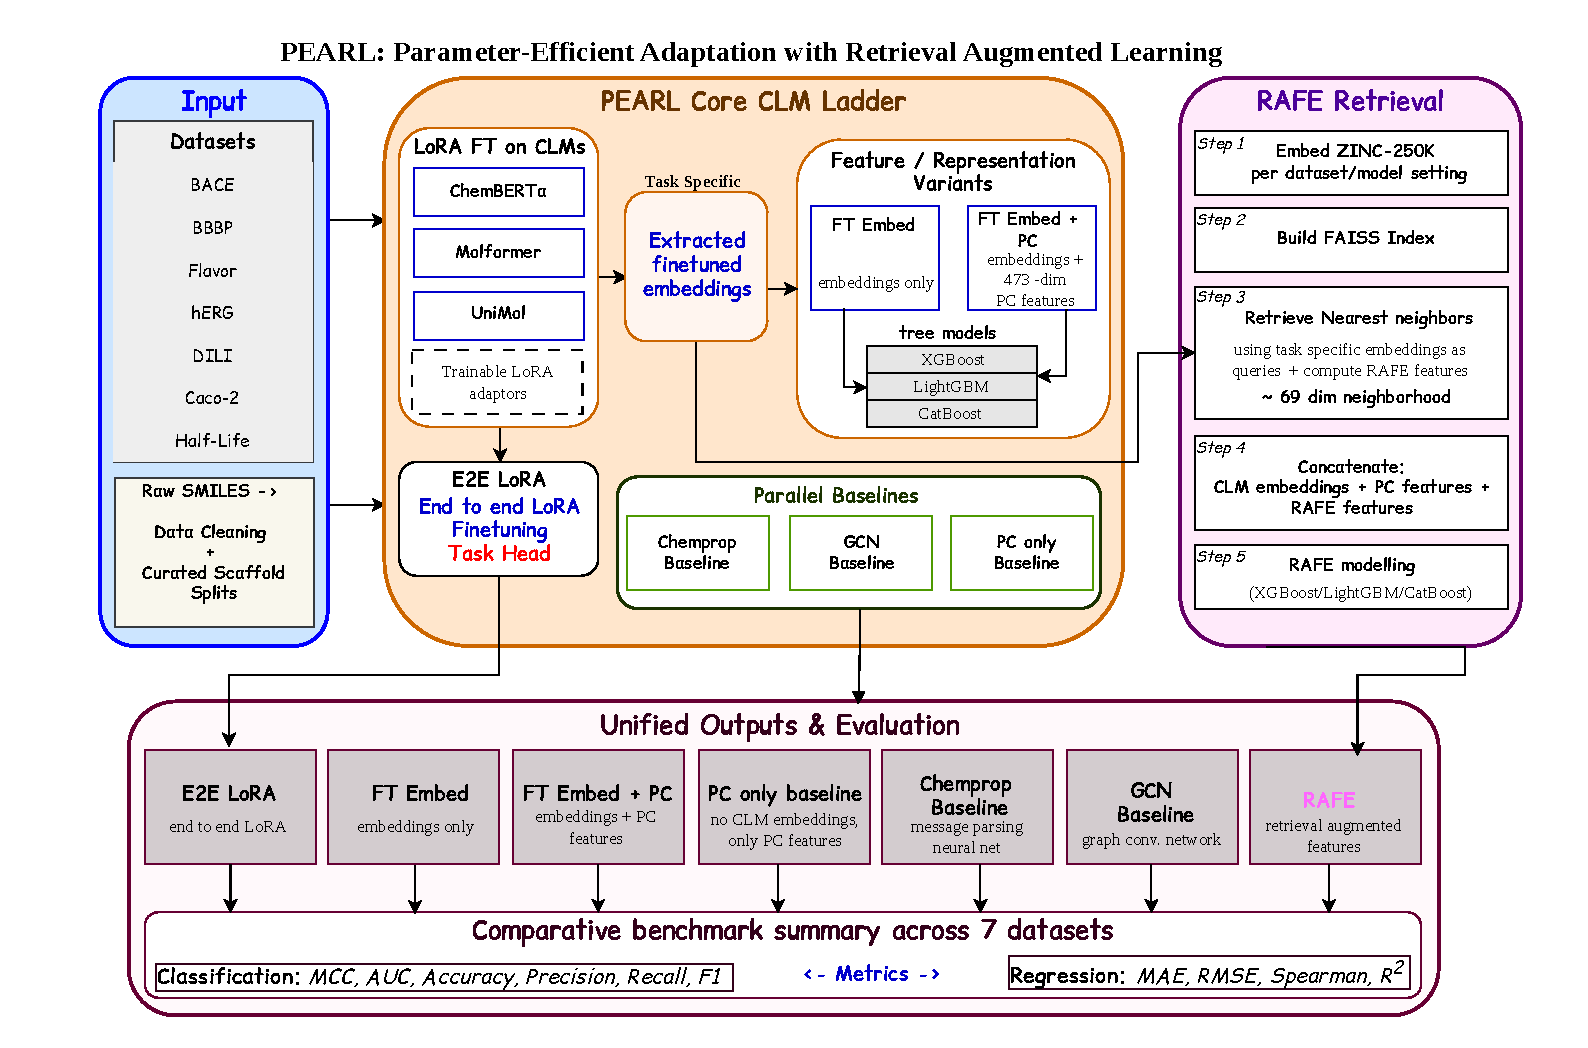
\includegraphics[width=0.99\textwidth]{PEARL_HM_Workflow_v2.pdf}
  \caption{PEARL workflow. Molecules are processed by one of three CLM families (ChemBERTa, MolFormer, Uni-Mol) with LoRA adapters. Task-specific embeddings are fused with molecular PC features and ZINC-250k retrieval features, then passed to tree-based classifiers/regressors. Uni-Mol also encodes 3D ETKDGv3 conformers via an SE(3) representation. The ladder spans both classification and regression targets (including Caco-2, Half-Life) and is benchmarked against in-house Chemprop/GCN/PC-only baselines run under the same protocol.}
  \label{fig:workflow}
\end{figure*}

%% =====================================================================
\section{Related Work}\label{sec:related_work}

\subsection{Molecular Property Prediction}\label{sec:related_mpp}
ChemBERTa~\cite{chithrananda2020chemberta} and ChemBERTa-2~\cite{ahmad2022chemberta2} adapted BERT-style masked language modelling to SMILES, establishing the template for CLM pretraining on large molecular corpora. MolFormer~\cite{ross2022molformer} scaled this to $1.1\times10^9$ molecules using linear attention. Uni-Mol~\cite{zhou2023unimol} departed from SMILES by operating on explicit 3D atomic coordinates via an SE(3)-equivariant transformer, achieving state-of-the-art results on MoleculeNet through full finetuning. Multi-modal models such as MolT5~\cite{edwards2022molt5}, nach0~\cite{livne2024nach0}, and Omni-Mol~\cite{hu2025omnimol} integrate SMILES, graphs, and natural language, but systematic evaluation under parameter-efficient conditions remains limited. Other work adds geometric or chemical knowledge to the representation. GEM~\cite{fang2022geometry} encodes bond lengths and angles in a geometry-enhanced graph network. KPGT~\cite{li2023kpgt} pretrains a graph transformer with knowledge-guided molecular descriptors. LiTENexus~\cite{su2026litenexus} injects quantum-chemical information into a physics-informed operator, and a recent survey and benchmark~\cite{li2026survey} compares deep-learning approaches to property prediction in the foundation-model era. These studies change the representation or the pretraining objective. PEARL instead keeps the pretrained models fixed except for low-rank adapters and asks how much extra information, such as descriptors or a retrieved neighborhood, helps a downstream tree model.

On the graph side, Chemprop~\cite{yang2019chemprop}, AttentiveFP~\cite{xiong2020attentivefp}, GROVER~\cite{rong2020grover}, and Mole-BERT~\cite{xia2023molecbert} all show how much graph-based molecular representations can offer. Instead of taking those numbers from the original papers (Supplementary Section~S5), \textbf{PEARL re-trains Chemprop and a GCN in-house} on all seven datasets, with the same scaffold split, preprocessing and evaluation protocol as every other method. The TDC~\cite{huang2021tdc} ADMET Group provides curated, leaderboard-tracked hERG~\cite{wang2016herg}, DILI~\cite{xu2019dili}, Caco-2~\cite{wang2016caco2}, and half-life~\cite{obach2008half} datasets, which broaden PEARL beyond MoleculeNet-era classification tasks and include regression targets.

\subsection{Parameter-Efficient Fine-Tuning (PEFT)}\label{sec:related_peft}
LoRA~\cite{hu2021lora} introduced low-rank weight updates for large language models; PEFT methods have since been evaluated for molecular tasks. Balne et al.~\cite{balne2024peft} and Xu et al.~\cite{xu2023peftreview} survey PEFT strategies broadly, including adapter layers, prefix tuning, and LoRA, while Fu et al.~\cite{fu2023effectiveness} assess their effectiveness in NLP. The work closest to ours is EffiChem~\cite{harod2025effichem}, which shows that LoRA-based adaptation of 1D CLMs (ChemBERTa, MolFormer) can be efficient for molecular property prediction.

PEARL extends this work in three ways. First, it adds Uni-Mol, a 3D SE(3)-equivariant model, and compares 1D SMILES-based and 3D geometry-aware CLMs under LoRA on identical scaffold splits. Second, it adds RAFE, which augments frozen CLM embeddings with label-free neighborhood features from an external library. Third, it trains in-house GNN, fingerprint and PC-only baselines and extends the ladder to regression tasks. We did not find a prior study that combines these elements under one protocol, but we make no claim about unpublished work.

\subsection{Retrieval-Augmented Generation (RAG)}\label{sec:related_rag}
Generative RAG~\cite{lewis2020rag} conditions a language model on retrieved documents; molecular analogues typically retrieve labeled training-set molecules as auxiliary signals, introducing leakage and a small retrieval pool. KPGT~\cite{liu2022kpgt} injects knowledge-graph attributes into graph-transformer pretraining but retrieval occurs at pretraining time from the training corpus itself. RAFE differs in three ways. It retrieves from a fixed external corpus (ZINC-250k) at inference time. It extracts label-free physicochemical statistics as tree-model features. It applies to any CLM family without retraining.

%% =====================================================================
\section{Materials and Methods}\label{sec:pearl_arch}
This section describes the seven benchmark datasets, the three CLM backbones that the PEARL framework builds on, and the two mechanisms that PEARL adds: parameter-efficient LoRA adaptation and RAFE retrieval augmentation. Together they define how PEARL adapts and enriches the backbones for downstream property prediction.

\subsection{Datasets}\label{sec:datasets}
PEARL is evaluated on seven molecular property prediction datasets that, taken together, span binary classification, multi-class classification, and regression, and range in size from a few hundred to over fifteen thousand compounds (Table~\ref{tab:dataset_summary}). Three are MoleculeNet-era classification benchmarks; the remaining four come from the TDC ADMET Group and add regression targets and a different (70:10:20) split convention, described below.

The \textbf{Blood-Brain Barrier Penetration (BBBP)} dataset was originally curated in~\cite{martins2012bayesian} for predicting barrier permeability and contains over $2,000$ compounds with binary labels, integrated into the MoleculeNet~\cite{wu2018moleculenet} benchmark. Blood-brain barrier permeability is a standard early filter in CNS drug discovery, and BBBP's compounds and splits are sourced directly from the IBM MolFormer repository, where they underwent validity checks, duplicate removal, and class-ambiguity filtering before we used them.

The \textbf{Flavor Analysis and Recognition Transformer (FART)} dataset, introduced in~\cite{zimmermann2024fart}, is a multi-class taste prediction corpus of 15,025 compounds annotated as \textit{bitter}, \textit{sour}, \textit{sweet}, \textit{umami}, and \textit{undefined}. It is, by a wide margin, the largest and most class-imbalanced dataset in this study, and is the only multi-class task PEARL is benchmarked on.

The \textbf{BACE} dataset is part of MoleculeNet~\cite{wu2018moleculenet} and contains experimentally measured binding results for 1,513 inhibitors of human $\beta$-secretase~1 (BACE-1), with binary activity labels. For all three of these MoleculeNet-era datasets, splits were curated using the DeepChem reference implementation~\cite{ramsundar2019deep}, which we use as-is rather than re-splitting the data ourselves, so that results remain comparable to prior work reporting on the same splits.

\textbf{TDC ADMET Group datasets:} Four datasets come from the Therapeutics Data Commons (TDC) ADMET Group~\cite{huang2021tdc}, chosen to broaden PEARL's task coverage beyond MoleculeNet-era binary/multi-class classification and to add regression targets. These include \textbf{hERG}~\cite{wang2016herg} (binary, cardiac ion-channel inhibition, 13{,}445 compounds), \textbf{DILI}~\cite{xu2019dili} (binary, drug-induced liver injury, 475 compounds), \textbf{Caco-2}~\cite{wang2016caco2} (regression, log apparent permeability, 906 compounds), and \textbf{Half-Life}~\cite{obach2008half} (regression, plasma half-life in hours, 667 compounds). All four are curated via TDC's standard scaffold split and undergo the same SMILES standardization, validity filtering, and duplicate-removal pipeline used for BACE, BBBP, and Flavor, so that no dataset in this study receives a bespoke preprocessing pipeline that could bias comparisons across the ladder. Half-Life also required IQR-based outlier removal in log1p space (bounds fit on the training split only, applied to all splits). Without it, a handful of extreme values (maximum $\approx 1200$h against a mean of $\sim$19h before filtering) would dominate the regression loss.

\subsubsection{Data Splits and Class Distribution}\label{sec:data_splits}
BBBP and BACE employ scaffold-based splits~\cite{ramsundar2019deep} using an 80:10:10 train/validation/test ratio. BBBP exhibits moderate class imbalance (78.8\% permeable in training); BACE is the most balanced dataset in this study, with $54.3\%$ inactive and $45.7\%$ active compounds, and its test set has $n\approx152$ molecules. The Flavor dataset uses the curated splits provided in~\cite{zimmermann2024fart}, with pronounced multi-class skew (sweet $41\%$, bitter $32\%$, sour $11\%$, umami $4\%$, undefined $12\%$) and $n_\text{test}=2{,}254$.

The four TDC ADMET datasets instead use TDC's scaffold split (70:10:20 train/valid/test, the TDC ADMET Group default). hERG's test set ($n=2{,}690$) is class-imbalanced toward inhibitors ($\sim$70\%); DILI is the smallest classification dataset in this study ($n_\text{test}=96$), so its bootstrapped CIs are correspondingly the widest among the binary tasks; Caco-2 ($n_\text{test}=182$) and Half-Life ($n_\text{test}=133$) are both small regression sets, motivating the same bootstrapped-CI discipline applied throughout this study.

\begin{table*}[!ht]
\centering
\caption{Structural summary of the seven PEARL benchmark datasets.}
\label{tab:dataset_summary}
\resizebox{0.9\textwidth}{!}{
\begin{tabular}{lllll}
\toprule
Dataset & Task type & \# Compounds & Split (train:val:test) & Primary metric \\
\midrule
BACE       & Binary classification       & 1{,}513  & 80:10:10 ($n_\text{test}\approx152$)   & MCC \\
BBBP       & Binary classification       & $>$2{,}000 & 80:10:10                               & MCC \\
Flavor     & 5-class classification      & 15{,}025 & curated~\cite{zimmermann2024fart} ($n_\text{test}=2{,}254$) & MCC \\
hERG       & Binary classification       & 13{,}445 & 70:10:20 ($n_\text{test}=2{,}690$)      & MCC \\
DILI       & Binary classification       & 475      & 70:10:20 ($n_\text{test}=96$)           & MCC \\
Caco-2     & Regression (log permeability) & 906    & 70:10:20 ($n_\text{test}=182$)          & Spearman \\
Half-Life  & Regression (log1p, hours)   & 667      & 70:10:20 ($n_\text{test}=133$)          & Spearman \\
\bottomrule
\end{tabular}
}
\end{table*}

\subsection{Problem Formulation}\label{sec:problem_formulation}
Let $\mathcal{D} = \{(x_i, y_i)\}_{i=1}^{N}$ denote a molecular property dataset, where $x_i$ is the $i$-th molecule and $y_i$ is its task-specific label. A molecule is represented either as a SMILES string (ChemBERTa, MolFormer) or as an explicit 3D atomic coordinate set obtained via conformer generation (Uni-Mol). For binary classification tasks (BACE, BBBP, hERG, DILI), $y_i \in \{0,1\}$; for the multi-class Flavor task, $y_i \in \{1,\dots,5\}$; for regression tasks (Caco-2, Half-Life), $y_i \in \mathbb{R}$.

A pretrained CLM backbone $f_\theta : \mathcal{X} \rightarrow \mathbb{R}^{d}$ maps a molecule to a $d$-dimensional embedding ($d=384$ for ChemBERTa, $d=768$ for MolFormer, $d=2560$ for Uni-Mol's hybrid vector). PEARL learns a task-specific predictor $g_\phi$ such that
\begin{equation}
  \hat{y}_i = g_\phi\big(h(x_i)\big), \qquad h(x_i) = f_\theta(x_i) \,\Vert\, p(x_i) \,\Vert\, r(x_i),
\end{equation}
where $\Vert$ denotes concatenation, $p(x_i) \in \mathbb{R}^{473}$ is an optional vector of engineered physicochemical descriptors, and $r(x_i) \in \mathbb{R}^{60}$ is an optional RAFE feature vector obtained by retrieving the $k$ nearest neighbors of $x_i$ in an external corpus $\mathcal{Z}$ (ZINC-250k). $\theta$ is adapted parameter-efficiently via low-rank updates $\Delta\theta$ with $|\Delta\theta| \ll |\theta|$, and $\phi$ is optimized to minimize a task-appropriate loss $\mathcal{L}(\hat y_i, y_i)$: weighted cross-entropy or focal loss for classification, Huber loss for regression. PEARL's four operational modes, described next, correspond to different choices of which terms in $h(x_i)$ are active and whether $g_\phi$ is trained end-to-end with $f_\theta$ or on frozen embeddings.

\subsection{Base CLM Backbone Architecture}\label{sec:pretrained_clms}
\textbf{ChemBERTa-2}~\cite{ahmad2022chemberta2} builds upon ChemBERTa~\cite{chithrananda2020chemberta} via a RoBERTa-style architecture trained on $77$ million canonical SMILES from PubChem~\cite{kim2023pubchem}. Two pretraining strategies are used: Masked Language Modeling (MLM) and Multi-Task Regression (MTR) on $200$ molecular property tasks. We use the two 77M-parameter variants, denoted \textbf{ChemBERTa-77M~MLM} and \textbf{ChemBERTa-77M~MTR}, each producing 384-dimensional embeddings.

\textbf{MolFormer}~\cite{ross2022molformer} is a scalable CLM that learns representations from SMILES without 3D geometry. It uses a transformer with linear attention (FAVOR+)~\cite{choromanski2021rethinking}, rotary positional embeddings~\cite{heo2024rotary}, and efficient distributed training~\cite{isard2009distributed}, enabling pretraining on $1.1\times 10^{9}$ molecules from PubChem~\cite{kim2023pubchem} and ZINC20~\cite{irwin2020zinc20}. We use the \textbf{MolFormer-XL-10pct-both} variant ($\approx 46$M parameters, pretrained on $10\%$ of both datasets) with 768-dimensional embeddings.

\textbf{Uni-Mol}~\cite{zhou2023unimol} is a universal 3D molecular pre-trained model based on a SE(3)-equivariant Transformer with 15 attention layers. Unlike SMILES-based CLMs, Uni-Mol accepts \emph{explicit 3D atomic coordinates} generated via RDKit ETKDGv3 conformer embedding followed by MMFF94 force-field minimization. This geometry-aware design gives Uni-Mol inductive biases suited to structure-dependent properties such as receptor binding affinity. For PEARL, each molecule is represented as a \textbf{2560-dimensional hybrid vector}: a 512-dimensional CLS token from the SE(3)-Transformer concatenated with 2048-dimensional Morgan ECFP4 fingerprints (radius $= 2$), combining 3D structural awareness with explicit 2D topological information.

\subsection{Parameter-Efficient Adaptation (LoRA)}\label{sec:lora}
Low-Rank Adaptation (LoRA)~\cite{hu2021lora} introduces two trainable low-rank matrices $\mathbf{B} \in \mathbb{R}^{d \times r}$ and $\mathbf{A} \in \mathbb{R}^{r \times d}$ alongside frozen pretrained weight matrices $\mathbf{W} \in \mathbb{R}^{d \times d}$ in the attention layers, where $r \ll d$ is the rank hyperparameter. The weight update is:
\begin{equation}
  \mathbf{W}' = \mathbf{W} + \Delta\mathbf{W}, \quad \Delta\mathbf{W} = \frac{\alpha}{r}\,\mathbf{B}\mathbf{A},
\end{equation}
where $\alpha$ is the LoRA scaling factor. Matrix $\mathbf{A}$ is initialized with the Kaiming-uniform scheme and $\mathbf{B}$ with zeros, so that $\Delta\mathbf{W}=0$ at the start and adaptation begins from the pretrained representation.

\subsubsection{LoRA for ChemBERTa and MolFormer}
LoRA adapters are applied to the query ($\mathbf{W}^Q$), key ($\mathbf{W}^K$), and value ($\mathbf{W}^V$) projection matrices of each attention layer (see Figure \ref{fig:lora-architecture}). All other parameters are frozen. Hyperparameter search covers rank $r \in \{4, 8, 16, 32, 64\}$, LoRA scaling $\alpha \in \{8, 16, 32, 64, 128\}$, and dropout $\in \{0.0, 0.1, 0.2\}$.

\subsubsection{LoRA for Uni-Mol}
The version of Uni-Mol employs a fused attention projection, where the query, key, and value transformations are combined into a single linear layer (\texttt{in\_proj}) rather than separate $\mathbf{W}^Q$, $\mathbf{W}^K$, and $\mathbf{W}^V$. Consequently, LoRA is applied directly to this unified projection module across all self-attention layers. Specifically, LoRA adapters are injected into the \texttt{in\_proj} weights (and \texttt{out\_proj} when available), enabling parameter-efficient fine-tuning without modifying the full backbone. The rank $r$ of the low-rank decomposition is selected from $\{4, 8, 16, 32\}$, while the scaling factor $\alpha$ is chosen from $\{8, 16, 32, 64\}$.

\begin{figure}[!htb]
  \centering
  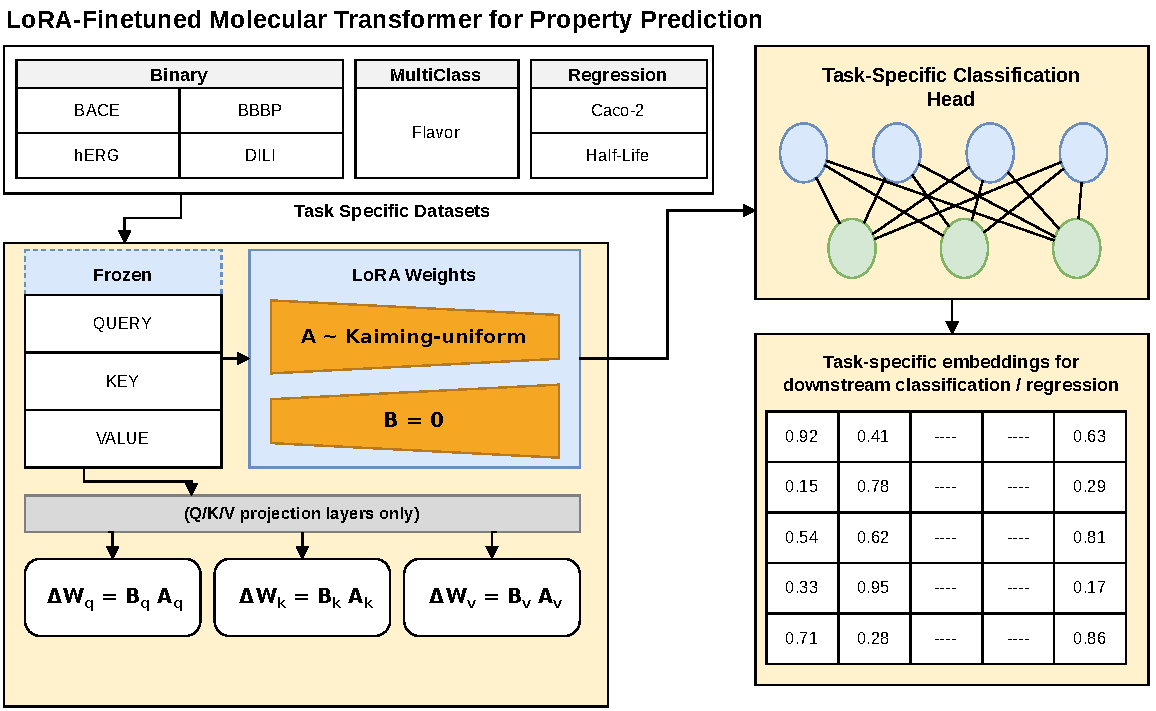
\includegraphics[width=0.99\textwidth]{LoRA_FineTuning_v3.pdf}
  \caption{Low-Rank Adaptation (LoRA) Architecture. A low-rank adaptation framework fine-tunes frozen transformer weights (Q/K/V layers) using trainable low-rank matrices (A, B), enabling efficient adaptation to task-specific molecular datasets including binary (hERG, DILI), multi-class (Flavor), and regression (Caco-2, Half-Life) targets.}
  \label{fig:lora-architecture}
\end{figure}
Conformers for all dataset molecules are generated once before the hyperparameter sweep and cached, avoiding redundant ETKDGv3 calls during hyperparameter optimization. We use necessary flags to prevent conformer generation failures for metal-coordinated SMILES. Figure~\ref{fig:lora-architecture} illustrates how LoRA finetuning is implemented within our framework. All models use AdamW with cosine-annealing learning rate schedules; the encoder (LoRA adapters) receives the base learning rate while the classification/regression head receives $5\times$ the base rate. Gradient clipping ($\text{max\_norm} = 1.0$) is applied over all parameters, and early stopping monitors validation MCC (classification) or validation RMSE (regression) with patience of 5 epochs. Bayesian hyperparameter optimization with WandB sweeps ($20$-$30$ trials per dataset) optimizes for the corresponding validation metric.

\subsection{Retrieval-Augmented Learning: the RAFE Component}\label{sec:rafe}

\subsubsection{Design Rationale and External Knowledge Base}\label{sec:zinc_rationale}
Naive retrieval-augmented approaches retrieve nearest neighbors from the task-specific training set and use their labels as auxiliary features. This introduces three problems: a small retrieval pool ($\sim$500-15,000 molecules depending on dataset), training-set leakage, and circular dependencies between the retrieval space and prediction target.

Unlike generative RAG~\cite{lewis2020rag}, where retrieved passages are injected into a language model prompt, RAFE does not pass retrieved content to any neural model. Retrieved ZINC-250k neighbors serve solely as a source of label-free physicochemical statistics (logP, QED, SAS distributions, structural similarity) that are featurized and concatenated with the molecular embedding before a tree-based model. The ``retrieval-augmented'' framing refers to the use of an external knowledge base at inference time, not to in-context generation.

PEARL addresses all three problems by using \textbf{ZINC-250k}~\cite{gomez2018automatic} as the retrieval corpus, i.e.\ a curated subset of $249,455$ drug-like molecules from the ZINC database~\cite{irwin2020zinc20} with no overlap with any training, validation, or test split, across all seven PEARL datasets. Each ZINC-250k molecule carries three physicochemical properties: lipophilicity (logP), Quantitative Estimate of Drug-likeness (QED $\in [0,1]$), and Synthetic Accessibility Score (SAS $\in [1,10]$).

ZINC-250k is chosen as the retrieval corpus for four complementary reasons:
\begin{enumerate}
  \item \textbf{Scale and diversity:} $249,455$ drug-like molecules span a broad region of chemical space, providing a dense and representative neighborhood for any query molecule from any of the seven PEARL datasets (the largest, hERG, has 13,445 compounds; the smallest, DILI, has 475).
  \item \textbf{Zero leakage:} ZINC-250k has no label overlap with any training, validation, or test split used in this study. Retrieved neighbors cannot carry prediction targets, eliminating the circular dependency that plagues training-set retrieval.
  \item \textbf{Label-free property signal:} logP, QED, and SAS are computed directly from SMILES without biological assay data. Their distributions in the local neighborhood of a query molecule characterize its physico-chemical environment in a way that is complementary to the molecule's own PC features and to the CLM's learned representation.
  \item \textbf{Model-family independence:} ZINC-250k is embedded independently by each finetuned CLM variant (ChemBERTa, MolFormer, Uni-Mol) and for each dataset, yielding model- and dataset-specific FAISS indices. RAFE features are therefore always expressed in the same geometric space as the query molecule's embedding.
\end{enumerate}

\subsubsection{Vector Indexing with FAISS}\label{sec:vector_faiss}
For each of the seven datasets, ZINC-250k molecules are re-embedded using that dataset's task-specific finetuned model variants. For binary/multi-class tasks, this means six SMILES-based variants (ChemBERTa-MLM $\times$ 2 loss, ChemBERTa-MTR $\times$ 2 loss, MolFormer $\times$ 2 loss) plus two Uni-Mol variants (FL and WL). For the two regression datasets, only a single Huber-loss variant is finetuned per CLM family, yielding three SMILES-based and one Uni-Mol variant.

SMILES-based embeddings are 768-dimensional CLS tokens; Uni-Mol embeddings are 2560-dimensional hybrid vectors (512-dim SE(3)-Transformer CLS concatenated with 2048-dim ECFP4 fingerprints). Embeddings are L2-normalized and indexed with FAISS \texttt{GpuIndexFlatIP}~\cite{johnson2021faiss}, a GPU-accelerated exact cosine-similarity search that achieves sub-2~ms query latency at 249k$\times$768 on a single GPU. The FAISS indices are serialized as CPU \texttt{IndexFlatIP} files for portable, fast retrieval.

\subsubsection{Chemical Neighborhood Feature Extraction}\label{sec:feature_extraction}
For every molecule in every split (train, validation, test), each FAISS index is queried by cosine similarity for the $k \in \{10, 20\}$ nearest ZINC-250k neighbors ($k$ fixed across all seven datasets; Section~\ref{sec:rafe_effectiveness} shows that the result does not depend on $k$). Four feature groups are extracted:
\begin{itemize}
  \item[\textbf{(a)}] physico-chemical neighborhood profile (18 features: mean/std of logP, QED, SAS at $k=10,20$, plus similarity-weighted means);
  \item[\textbf{(b)}] neighborhood density (5 features: nearest-neighbor similarity, mean/std of $k$-neighbor similarity at $k=10,20$);
  \item[\textbf{(c)}] embedding centroid features (34 features: PCA-32 compression of the $k=10$ neighbor centroid, fit on train only, plus similarity-to-centroid and centroid spread via standard deviation);
  \item[\textbf{(d)}] Tanimoto structural similarity (3 features: Morgan-fingerprint Tanimoto to the top-1 and top-5 neighbors, plus Murcko-scaffold overlap fraction in the top-10).
\end{itemize}
Together these four groups yield a 60-dimensional RAFE feature vector (18 + 5 + 34 + 3) per molecule, concatenated as: [$\text{CLM embeddings} \mid \text{PC features (473-dim)} \mid \text{ZINC RAFE features}$] as depicted in Figure \ref{fig:rafe}.

\begin{figure}[!ht]
  \centering
  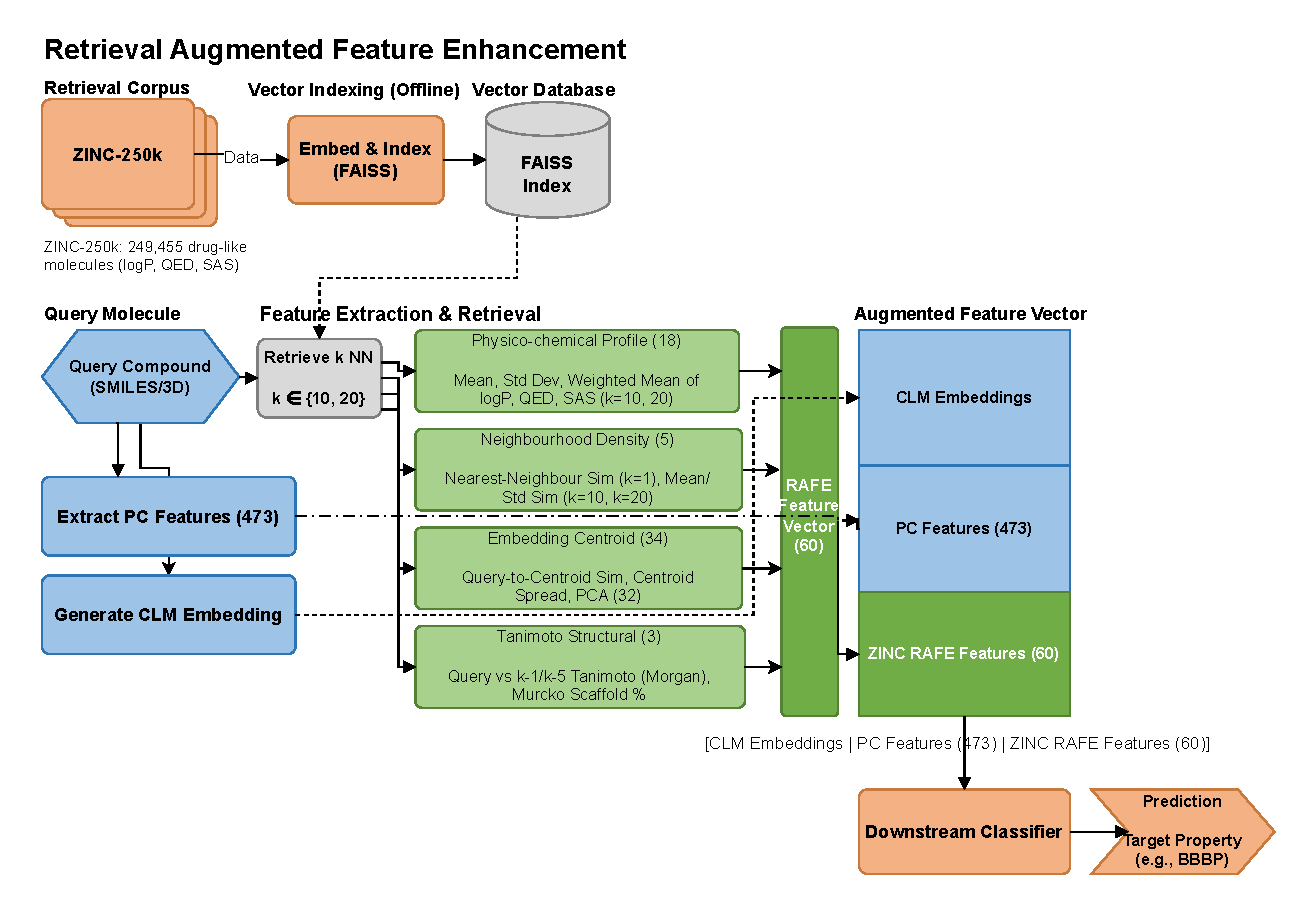
\includegraphics[width=0.99\textwidth]{RAFE_Framework_v2.pdf}
  \caption{Retrieval-Augmented Feature Enhancement (RAFE) pipeline. A query molecule is embedded by a task-specific finetuned CLM; the embedding retrieves $k$ nearest chemical neighbors from the ZINC-250k FAISS index (re-built independently per dataset). Four feature groups are extracted (physico-chemical neighborhood profile, density/isolation, embedding centroid, Tanimoto similarity), yielding a 60-dim RAFE vector concatenated with the CLM embedding and PC features for tree-based classification or regression.}
  \label{fig:rafe}
\end{figure}

\subsection{The PEARL Framework: Operational Ladder and Baselines}\label{sec:pearl_ladder}
Having introduced its three backbone CLMs, its LoRA adaptation mechanism, and its RAFE retrieval component, we can now describe how the PEARL framework assembles them. PEARL defines four operational modes that form a progressive evaluation ladder, applicable to both classification and regression targets:

\textbf{(a)~End-to-End (E2E) LoRA finetuning:} The CLM backbone (ChemBERTa, MolFormer, or Uni-Mol) with LoRA adapters and a task-specific head is optimized end-to-end for each downstream task. For binary tasks, the head is a dense layer with sigmoid activation; for multi-class tasks, a dense layer with softmax; for regression tasks (Caco-2, Half-Life), a single linear output unit trained with Huber loss.

\textbf{(b)~Finetuned Embedding Prediction (FT~Embed):} Task-specific embeddings are extracted from the finetuned model. For MolFormer, the CLS token passes through two dense layers with GELU activation (768-dim output). For ChemBERTa, the CLS token passes through a dense layer with tanh activation (384-dim). For Uni-Mol, the CLS token is concatenated with ECFP4 fingerprints (2560-dim). These embeddings train Optuna-tuned~\cite{akiba2019optuna} tree-based classifiers (XGBoost / LightGBM / CatBoost) or, for the two regression datasets, their regressor counterparts.

\textbf{(c)~FT~Embed $+$ PC (Physicochemical Feature Fusion):} The FT~Embed vector is concatenated with 473~domain-specific physicochemical (PC) features: 148 RDKit molecular descriptors, 30 graph-based features (NetworkX v3.5.2), 128-bit Morgan fingerprints, and 167-bit MACCS keys (RDKit v2025.09.4). This combined vector trains the same tree-based models without any retrieval from external databases. A full description of engineered features is provided in Supplementary Table~S1.

\textbf{(d)~Retrieval-Augmented Feature Enhancement (RAFE):} RAFE augments the FT~Embed $+$ PC feature vector with ZINC-250k chemical neighborhood features (60-dim; Section~\ref{sec:rafe}), yielding the full feature vector [$\text{CLM embeddings} \mid \text{PC features (473-dim)} \mid \text{ZINC-250k RAFE features}$], passed to the same Optuna-tuned tree-based models.

\textbf{Baselines run in-house under the identical protocol, outside the ladder:} \textbf{PC-only} trains the same tree-model family directly on the 473-dim PC vector, with \emph{no} CLM component, isolating how much of the ladder's performance is attributable to the CLM. \textbf{Chemprop}~\cite{yang2019chemprop} (D-MPNN) and a \textbf{GCN} (GINConv-based, hand-rolled, atom/bond-featurized) are both trained end-to-end on the molecular graph, on the same scaffold split, with the same Optuna-style hyperparameter search budget and the same bootstrapped-CI evaluation as every CLM-based method above.

\subsection{Loss Functions for Class Imbalance and Regression}\label{sec:loss_functions}
Three loss functions address class imbalance (classification) or robust regression, implemented via a custom extension of the HuggingFace \texttt{Trainer}.

\noindent \textbf{Weighted cross-entropy (WL):} $\mathcal{L}_{\text{WL}} = -\sum_{i=0}^{C-1} w_i y_i \log\hat{y}_i$, where $w_i = 1 - f_i$ (inverse class frequency). This gives the minority class higher loss contribution and is most effective for datasets like BACE and Flavor.

\noindent\textbf{Focal loss (FL):} $\mathcal{L}_{\text{FL}} = -\alpha_c (1 - \hat{p}_c)^\gamma \log\hat{p}_c$ for the true class $c$, with $\gamma = 2$ and per-class weights $\alpha_c = 1 - f_c$ (one minus the training-set class frequency), which down-weights well-classified examples to focus learning on hard-to-classify boundary cases. This excels on heavily imbalanced and challenging classification tasks. hERG and DILI both use FL and WL sweeps, matching the same protocol used for BACE, BBBP, and Flavor.

\noindent\textbf{Huber loss (regression):} $\mathcal{L}_{\text{Huber}}(y, \hat y) = \begin{cases}\tfrac{1}{2}(y-\hat y)^2 & |y - \hat y| \le \delta \\ \delta(|y-\hat y| - \tfrac12 \delta) & \text{otherwise}\end{cases}$, with $\delta = 1.0$. Huber loss is used for both regression targets. It combines MSE's smoothness near zero error with MAE's robustness to the outlier-prone tail of half-life measurements (the Half-Life target is also log1p-transformed before the Huber loss is applied, and predictions are inverse-transformed before evaluation).

\subsection{Tree-Based Prediction Models}\label{sec:tree_models}
The final prediction stage employs XGBoost~\cite{chen2016xgboost}, LightGBM~\cite{ke2017lightgbm}, and CatBoost~\cite{prokhorenkova2018catboost}, in their classifier or regressor form as appropriate. These algorithms handle high-dimensional mixed-type feature vectors, provide built-in feature importance, and are robust to outliers. Hyperparameters were tuned with Optuna~\cite{akiba2019optuna} ($20$ trials for each configuration) on the training split only, maximizing MCC (classification, stratified 5-fold cross-validation) or minimizing RMSE (regression, 5-fold cross-validation). Class-weighting strategies address imbalance for classification tasks (\texttt{scale\_pos\_weight}, \texttt{class\_weight="balanced"}, \texttt{auto\_class\_weights="Balanced"} for XGBoost/LightGBM/CatBoost respectively); regression targets are otherwise unweighted.

%% =====================================================================
\section{Experimental Setup and Benchmarking}\label{sec:experimental_setup}
The seven datasets, their splits, and class/label distributions used throughout this benchmark are described in Section~\ref{sec:datasets} (Table~\ref{tab:dataset_summary}).

\subsection{Baseline Models}\label{sec:baselines}
PEARL's four operational modes are compared against three in-house baselines run under the identical scaffold split, preprocessing, and evaluation protocol: \textbf{PC-only} (no CLM, no LoRA, no retrieval), \textbf{Chemprop}~\cite{yang2019chemprop} (D-MPNN), and a hand-rolled \textbf{GCN} (GINConv-based). We also train the same tree models on conventional fingerprints and descriptors (ECFP4, ECFP6, MACCS, ECFP4$+$MACCS and the RDKit descriptor set), under the same splits and tuning. On the three MoleculeNet-era datasets (BACE, BBBP, Flavor), for which comparable literature numbers exist, PEARL is compared against published external baselines: Chemprop~\cite{yang2019chemprop}, GROVER~\cite{rong2020grover}, AttentiveFP~\cite{xiong2020attentivefp}, Mole-BERT~\cite{xia2023molecbert}, and the original Uni-Mol and MolFormer full-finetuning results (Section~\ref{sec:external_comparison}). The four TDC ADMET Group tasks have no comparable external LoRA/RAFE literature baseline, so their comparison is entirely in-house.

\subsection{Evaluation Protocol, Model Selection and Statistics}\label{sec:eval_protocol}
\paragraph{Metrics.} For classification we report accuracy, area under the ROC curve (AUC), Matthews correlation coefficient (MCC), precision, recall and F1 (macro and micro); MCC is the primary ranking metric because it is robust to class imbalance. For the two regression datasets (Caco-2, Half-Life) we report R\textsuperscript{2}, mean absolute error and Spearman rank correlation, and rank by Spearman.

\paragraph{Tuning and model selection.} All tree models are tuned on the training split only: 20 Optuna trials per configuration, 5-fold cross-validation, and balanced sample weights for classification. The test split is evaluated once per fitted model and is never used for tuning. LoRA fine-tuning uses the fixed training and validation splits (the validation split for monitoring and early stopping), not cross-validation. Configurations (embedding model, loss, tree model and stage) are compared on the test set, as is usual for benchmarks. Because the best configuration is selected on the same test set, its score is optimistic. We therefore report five-seed means next to every single-run best value, and the paired difference between the best and the runner-up configuration (Table~\ref{tab:best_configs}).

\paragraph{Seeds and paired statistics.} Every downstream arm is run with five seeds (42 to 46). The seed sets the Optuna sampler, the cross-validation shuffle and the model initialization. Two arms are compared with a paired bootstrap on identical test molecules: in each of 3{,}000 resamples the test molecules are resampled once, the metric difference is computed for each seed and averaged over seeds, and the 2.5th and 97.5th percentiles give a 95\% interval. We call a difference significant when this interval excludes zero. The 10{,}000-resample standard errors in the single-run tables and in Figure~\ref{fig:results_summary} are descriptive. Comparisons between configurations that share a test set (for example Wilcoxon tests over matched configurations) are likewise descriptive.

\paragraph{Scope of the variability estimates.} The seeds cover the downstream tree stage. LoRA fine-tuning, the re-embedding of ZINC-250k and the end-to-end LoRA, Chemprop and GCN baselines are single runs, so the intervals are lower bounds on the total variability. The new experiments ran XGBoost on GPU, so absolute values differ slightly from the original CPU runs; arms are therefore always compared within one experiment.

\paragraph{Implementation.} All training uses AdamW with cosine-annealing learning rate schedules. LoRA hyperparameters were searched with WandB sweeps ($20$-$30$ trials per dataset). Hardware, environment specification and wall-clock timings are documented in the code repository (\url{https://github.com/raghvendra5688/PEARL}).

%% =====================================================================
\section{Results and Discussion}\label{sec:results_discussion}

We organize the results around the four PEARL operational modes described in Section~\ref{sec:pearl_ladder}, plus the in-house baselines (PC-only, Chemprop, GCN) run identically across all seven datasets: (i)~\textbf{E2E LoRA}, end-to-end LoRA finetuning of the CLM backbone; (ii)~\textbf{FT Embed}, Optuna-tuned tree models on frozen finetuned embeddings; (iii)~\textbf{FT Embed $+$ PC}, FT Embed augmented with 473 physicochemical features; and (iv)~\textbf{RAFE}, FT Embed $+$ PC augmented with ZINC-250k neighborhood features. The per-dataset tables (Section~\ref{sec:main_results}) give the best configuration of each mode from single runs. Sections~\ref{sec:controlled} to~\ref{sec:fingerprints} then repeat the comparison under controlled conditions and on five-seed means, and Sections~\ref{sec:rafe_effectiveness} to~\ref{sec:efficiency} examine H2, H3 and H1 in turn.

\subsection{Main Benchmarking Results}\label{sec:main_results}

\subsubsection{Sequence of Comparisons}\label{sec:comparison_sequence}
The four PEARL modes form a ladder that isolates the contribution of each component. \textbf{PC-only} (no CLM) sets the floor: a CLM-based method that does not beat it has not shown that its added complexity pays off on that dataset. \textbf{E2E LoRA} is the reference for end-to-end gradient flow through the backbone. \textbf{FT Embed} measures what the embedding contributes alone, and any gap to E2E LoRA reflects information recoverable only through end-to-end training. \textbf{FT Embed $+$ PC} isolates the physicochemical features, independent of retrieval. \textbf{RAFE} measures the added value of ZINC-250k neighborhood context: a gain over FT Embed $+$ PC would suggest information beyond both the learned representation and the molecule's own physicochemical profile. \textbf{Chemprop and GCN}, run in-house on the identical split and protocol, are graph-based references that isolate explicit bond-graph message passing, independent of any CLM pretraining corpus.

The per-dataset tables below report single-run best configurations. Their standard errors are descriptive, because the best row of each mode is chosen on the test set. Formal comparisons use paired bootstrap intervals on identical test molecules (Section~\ref{sec:eval_protocol}) and are reported in Section~\ref{sec:controlled}. Figure~\ref{fig:results_summary} shows the single-run primary metric of every method on all seven datasets.

\begin{figure*}[!ht]
  \centering
  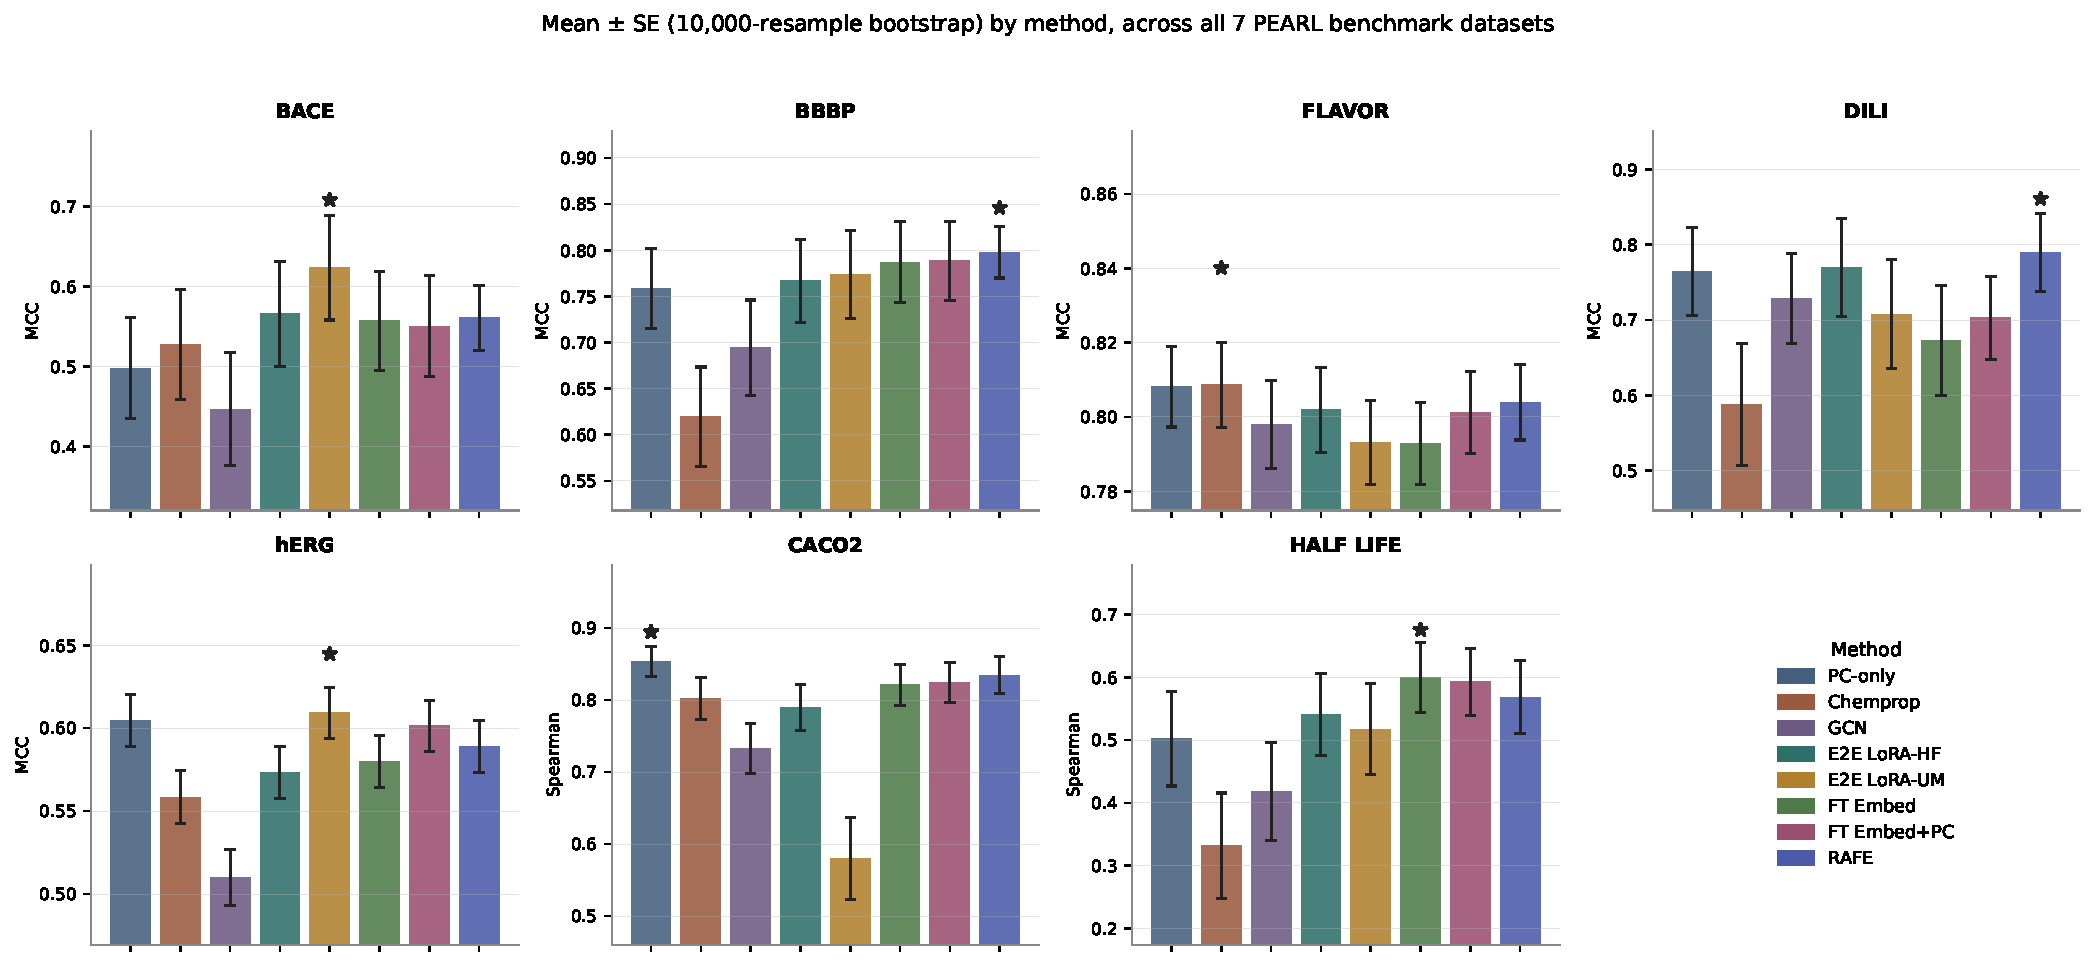
\includegraphics[width=0.99\textwidth]{results_summary_v2.pdf}
  \caption{Mean $\pm$ SE (10,000-resample bootstrap) of the primary ranking metric (MCC for classification, Spearman for regression) for every method across all seven PEARL benchmark datasets. Stars mark the point-estimate winner per dataset. Values are single runs of the best configuration of each method; the bars are descriptive and not a test of the difference.}
  \label{fig:results_summary}
\end{figure*}

\subsubsection{BBBP Dataset Results}
Table~\ref{tab:bbbp} lists the best configuration per modality and CLM family for BBBP (single runs). The highest value is RAFE with MolFormer-XL (FL~$+$~XGBoost; MCC$=0.798$, AUC$=0.940$, SE$=0.028$), ahead of E2E LoRA MolFormer FL (MCC$=0.767$, AUC$=0.929$) and Uni-Mol E2E LoRA WL (MCC$=0.774$, AUC$=0.943$). This single-run value is optimistic. The same configuration averages MCC$=\mBBBPRAFE \pm \sBBBPRAFE$ over five seeds, and FT Embed+PC with the same embedding and tree averages $\mBBBPFTPC \pm \sBBBPFTPC$ (single run: $\srBBBPFTPC$). Within the same tree, the two stages are indistinguishable (Table~\ref{tab:full_bbbp}). PC-only reaches MCC$=0.759$ in the original table and $\mBBBPPC$ over five seeds (best tree). The advantage of RAFE over the fine-tuned embedding alone is small ($+0.014$ on average over matched configurations, Wilcoxon $p=0.025$; Figure~\ref{fig:ladder}). In the controlled matrix, FT Embed+PC is $+0.054$ above PC-only with XGBoost (95\% interval $-0.017$ to $+0.130$), so we read BBBP as a dataset where fine-tuned embeddings tend to help over descriptors and RAFE adds no measurable benefit beyond them. Full per-embedding, per-loss results are in Supplementary Table~S2.

\begin{table*}[!ht]
\centering
\caption{Best performing configurations for each modality/baseline on BBBP. $^*$ denotes overall best by MCC. RAFE = FT~Embed~+~PC~+~ZINC-250k retrieval features. PC-only / Chemprop / GCN are run in-house on the identical split.}
\label{tab:bbbp}
\resizebox{0.95\textwidth}{!}{
\begin{tabular}{lllllrrrrrrr}
\toprule
Modality & CLM & Loss & ML & AUC & Acc & F1$_\text{mac}$ & F1$_\text{mic}$ & MCC & Prec & Rec & SE(MCC) \\
\midrule
PC-only    & --- & --- & LightGBM & 0.937 & 0.885 & 0.867 & 0.885 & 0.759 & 0.916 & 0.846 & 0.043 \\
Chemprop   & --- & --- & --- & 0.918 & 0.807 & 0.801 & 0.807 & 0.620 & 0.799 & 0.821 & 0.054 \\
GCN        & --- & --- & --- & 0.924 & 0.859 & 0.839 & 0.859 & 0.694 & 0.874 & 0.822 & 0.052 \\
\midrule
E2E LoRA   & MolFormer-XL & FL & --- & 0.929 & 0.891 & 0.874 & 0.891 & 0.767 & 0.913 & 0.856 & 0.045 \\
E2E LoRA   & Uni-Mol      & WL & --- & 0.943 & 0.896 & 0.887 & 0.896 & 0.774 & 0.890 & \textbf{0.885} & 0.048 \\
\midrule
FT Embed   & MolFormer-XL & FL & XGBoost & 0.935 & 0.901 & 0.888 & 0.901 & 0.787 & 0.914 & 0.873 & 0.044 \\
FT Embed+PC& MolFormer-XL & FL & LightGBM& 0.934 & 0.901 & 0.887 & 0.901 & 0.789 & 0.920 & 0.870 & 0.043 \\
\midrule
RAFE$^*$   & MolFormer-XL & FL & XGBoost & \textbf{0.940} & \textbf{0.906} & \textbf{0.895} & \textbf{0.906} & \textbf{0.798} & \textbf{0.918} & 0.881 & \textbf{0.028} \\
RAFE       & Uni-Mol      & FL & XGBoost & 0.928 & 0.891 & 0.872 & 0.891 & 0.773 & 0.927 & 0.850 & --- \\
\bottomrule
\end{tabular}
}
\end{table*}

\subsubsection{Flavor Dataset Results}
Table~\ref{tab:flavor} presents results on the multi-class Flavor dataset (single runs). RAFE (MolFormer-XL WL~$+$~CatBoost) reaches MCC$=0.804$ (AUC$=0.963$, Prec$=0.868$, Rec$=0.749$, SE$=0.010$), within one standard error of Chemprop (MCC$=0.809$, SE$=0.0115$) and PC-only (MCC$=0.808$, SE$=0.0108$). The test set is large ($n_\text{test}=2{,}254$), so the controlled comparison is informative: with XGBoost, RAFE is significantly below PC-only ($-0.027$, 95\% interval $-0.044$ to $-0.010$; Table~\ref{tab:controlled}), and with LightGBM and CatBoost the intervals include zero. The CLM ladder therefore does not clear the PC-only and GNN baselines on this dataset. Uni-Mol reaches MCC$=0.795$ with weighted loss, competitive with but below MolFormer, which suggests that 3D geometry adds little for taste prediction. \pending{five-seed values for Flavor} The full per-embedding, per-loss ablation is in Supplementary Table~S3.

\begin{table*}[t]
\centering
\caption{Best performing configurations on Flavor. Prec/Rec are macro-averaged; AUC is one-vs-rest macro ROC AUC.}
\label{tab:flavor}
\resizebox{0.95\textwidth}{!}{
\begin{tabular}{lllllrrrrrrr}
\toprule
Modality & CLM & Loss & ML & AUC & Acc & F1$_\text{mac}$ & F1$_\text{mic}$ & MCC & Prec & Rec & SE(MCC) \\
\midrule
PC-only    & --- & --- & XGBoost  & 0.972 & 0.890 & 0.761 & 0.890 & 0.808 & 0.733 & 0.798 & 0.0108 \\
Chemprop   & --- & --- & --- & 0.974 & \textbf{0.899} & \textbf{0.809} & \textbf{0.899} & \textbf{0.809} & 0.796 & 0.835 & 0.0115 \\
GCN        & --- & --- & --- & 0.973 & 0.893 & 0.814 & 0.893 & 0.798 & 0.834 & 0.800 & 0.0118 \\
\midrule
E2E LoRA   & MolFormer-XL & WL & --- & \textbf{0.975} & 0.892 & \textbf{0.809} & 0.892 & 0.802 & 0.802 & 0.817 & 0.0115 \\
\midrule
FT Embed   & MolFormer-XL & WL & LightGBM& 0.970 & 0.882 & 0.783 & 0.882 & 0.787 & 0.800 & 0.778 & 0.0111 \\
FT Embed+PC& MolFormer-XL & WL & CatBoost& 0.958 & 0.888 & 0.772 & 0.888 & 0.801 & 0.756 & 0.793 & 0.0111 \\
\midrule
RAFE       & MolFormer-XL & WL & CatBoost& 0.963 & 0.893 & 0.774 & 0.893 & 0.804 & \textbf{0.868} & 0.749 & 0.0102 \\
\bottomrule
\end{tabular}
}
\end{table*}

\subsubsection{BACE Dataset Results}
Table~\ref{tab:bace} compares key configurations on BACE. BACE remains the most challenging dataset here (MCC $< 0.65$ across all methods). Figure~\ref{fig:bace} compares the AUC and AUPR of Uni-Mol E2E LoRA with counterparts in the CLM ladder. \textbf{Uni-Mol with weighted loss gives the highest single-run value} (MCC$=0.623$, SE$=0.039$; AUC$=0.891$; Acc$=0.822$), $0.057$ above the next-best SMILES-based E2E LoRA (MolFormer-XL FL, MCC$=0.566$, SE$=0.066$) and $0.125$ above PC-only in the original table (MCC$=0.498$, SE$=0.063$). The bands of Uni-Mol and MolFormer FL overlap, so the gain over the best SMILES-based model is directionally consistent but not confirmed on this test set ($n=152$). The end-to-end model is a single run with its own prediction head, so we cannot attach a seed interval to it. The tree-based stages are weaker: the best five-seed means are $\mBACEFT$ (FT Embed), $\mBACEFTPC$ (FT Embed+PC) and $\mBACERAFE$ (RAFE) with MolFormer, against $\mBACEPC$ for PC-only. BACE-1 activity depends on three-dimensional ligand-receptor complementarity, which is consistent with the advantage of the 3D end-to-end model, but our data do not establish that mechanism (Section~\ref{sec:3d_ecfp}).

RAFE with MolFormer-XL (WL~+~LightGBM) achieves MCC$=0.561$, SE$=0.040$, intermediate between FT Embed (MCC$=0.557$) and E2E LoRA (MCC$=0.566$), and does not close the gap to Uni-Mol E2E LoRA. The full per-embedding, per-loss ablation results are reported in Supplementary Table~S4.

\begin{figure*}[!ht]
  \centering
  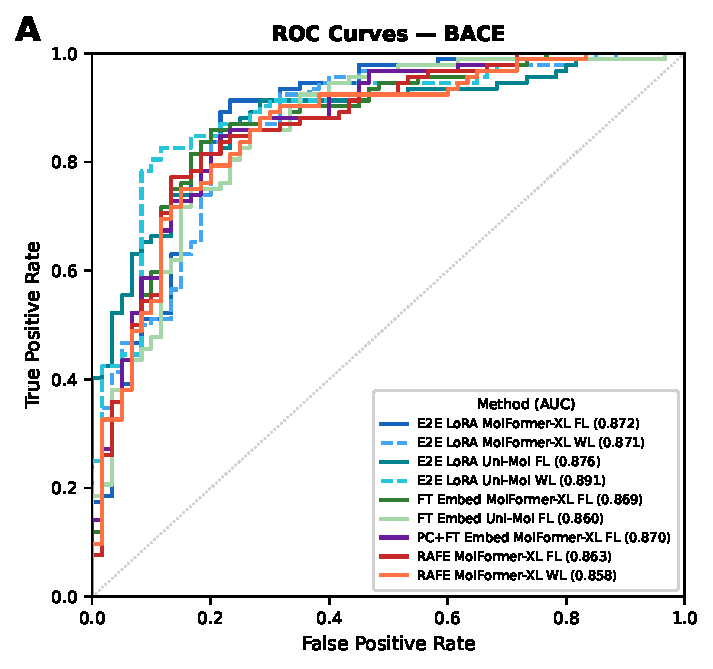
\includegraphics[width=0.49\textwidth]{bace_roc.pdf}
  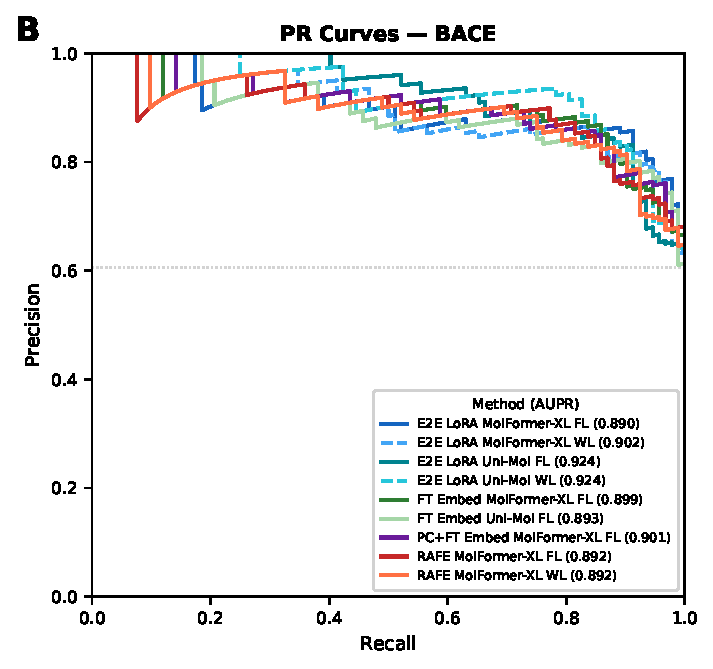
\includegraphics[width=0.49\textwidth]{bace_pr.pdf}
  \caption{ROC and precision-recall curves for BACE inhibitor prediction. Uni-Mol WL achieves the highest AUPR and overall MCC~$=0.623$.}
  \label{fig:bace}
\end{figure*}

\begin{table*}[ht]
\centering
\caption{Best configurations on BACE. $^*$ overall best by MCC.}
\label{tab:bace}
\resizebox{0.95\textwidth}{!}{
\begin{tabular}{lllllrrrrrrr}
\toprule
Modality & CLM & Loss & ML & AUC & Acc & F1$_\text{mac}$ & F1$_\text{mic}$ & MCC & Prec & Rec & SE(MCC) \\
\midrule
PC-only    & --- & --- & CatBoost & 0.850 & 0.724 & 0.723 & 0.724 & 0.498 & 0.746 & 0.751 & 0.063 \\
Chemprop   & --- & --- & --- & 0.855 & 0.763 & 0.759 & 0.763 & 0.528 & 0.758 & 0.770 & 0.068 \\
GCN        & --- & --- & --- & 0.795 & 0.717 & 0.714 & 0.717 & 0.447 & 0.719 & 0.729 & 0.071 \\
\midrule
E2E LoRA   & MolFormer-XL & FL & --- & 0.872 & 0.789 & 0.785 & 0.789 & 0.566 & 0.783 & 0.789 & 0.066 \\
E2E LoRA$^*$ & Uni-Mol    & WL & --- & \textbf{0.891} & \textbf{0.822} & \textbf{0.808} & \textbf{0.822} & \textbf{0.623} & \textbf{0.823} & \textbf{0.801} & \textbf{0.039} \\
\midrule
FT Embed   & MolFormer-XL & FL & CatBoost & 0.869 & 0.763 & 0.762 & 0.763 & 0.557 & 0.773 & 0.784 & 0.062 \\
RAFE       & MolFormer-XL & WL & LightGBM & 0.858 & 0.770 & 0.768 & 0.770 & 0.561 & 0.774 & 0.787 & 0.040 \\
\bottomrule
\end{tabular}
}
\end{table*}

\subsubsection{TDC ADMET Group Results}\label{sec:new_datasets}
This section reports results on the four TDC ADMET Group datasets. All four are evaluated with the same in-house PC-only, Chemprop, and GCN baselines as BACE/BBBP/Flavor.

\paragraph{hERG (Cardiac Ion-Channel Inhibition).} Table~\ref{tab:herg} shows results for hERG (single runs). Uni-Mol E2E LoRA (WL) has the highest value (MCC$=0.609$, AUC$=0.881$, SE$=0.0154$), narrowly ahead of PC-only (MCC$=0.604$, SE$=0.0157$), FT~Embed+PC (Uni-Mol FL~$+$~LightGBM, MCC$=0.602$, SE$=0.0154$) and RAFE (Uni-Mol FL~$+$~LightGBM, MCC$=0.589$, SE$=0.0155$). The test set is large ($n=2{,}690$), and the controlled comparison shows that RAFE is significantly below PC-only with all three trees (differences $-0.049$, $-0.033$ and $-0.056$ for XGBoost, LightGBM and CatBoost; Table~\ref{tab:controlled}). RAFE is significantly above the fine-tuned embedding alone only with LightGBM ($+0.011$). The full set of ablations is in Supplementary Table~S5. \pending{five-seed grid values for hERG}

\begin{table*}[!ht]
\centering
\caption{Best configurations on hERG (binary, cardiac ion-channel inhibition).}
\label{tab:herg}
\resizebox{0.95\textwidth}{!}{
\begin{tabular}{lllllrrrrrrr}
\toprule
Modality & CLM & Loss & ML & AUC & Acc & F1$_\text{mac}$ & MCC & Prec & Rec & SE(MCC) \\
\midrule
PC-only     & --- & --- & XGBoost  & 0.874 & 0.802 & 0.802 & 0.604 & 0.802 & 0.802 & 0.0157 \\
Chemprop    & --- & --- & ---      & 0.854 & 0.779 & 0.779 & 0.558 & 0.779 & 0.779 & 0.0160 \\
GCN         & --- & --- & ---      & 0.833 & 0.755 & 0.755 & 0.510 & 0.755 & 0.755 & 0.0168 \\
\midrule
E2E LoRA    & MolFormer-XL & WL & --- & 0.869 & 0.787 & 0.787 & 0.573 & 0.787 & 0.787 & 0.0155 \\
E2E LoRA$^*$& Uni-Mol      & WL & --- & \textbf{0.881} & \textbf{0.804} & \textbf{0.804} & \textbf{0.609} & \textbf{0.805} & \textbf{0.804} & \textbf{0.0154} \\
\midrule
FT Embed    & Uni-Mol & FL & LightGBM & 0.864 & 0.790 & 0.790 & 0.580 & 0.790 & 0.790 & 0.0158 \\
FT Embed+PC & Uni-Mol & FL & LightGBM & 0.871 & 0.801 & 0.801 & 0.602 & 0.801 & 0.801 & 0.0154 \\
RAFE        & Uni-Mol & FL & LightGBM & 0.871 & 0.794 & 0.794 & 0.589 & 0.794 & 0.795 & 0.0155 \\
\bottomrule
\end{tabular}
}
\end{table*}

\paragraph{DILI (Drug-Induced Liver Injury).} Table~\ref{tab:dili} shows results for DILI (single runs). RAFE (Uni-Mol FL~$+$~XGBoost) has the highest value (MCC$=0.790$, AUC$=0.875$, SE$=0.0515$), ahead of E2E LoRA (ChemBERTa-MTR WL, MCC$=0.770$) and PC-only (MCC$=0.765$, SE$=0.0581$). This single-run value does not hold up under repetition: with five seeds, the same configuration gives MCC$=\mDILIRAFE \pm \sDILIRAFE$, FT Embed+PC $\mDILIFTPC \pm \sDILIFTPC$ and PC-only $\mDILIPC$. The test set is small ($n=96$), so every interval is wide. What survives is a consistent benefit of RAFE over the fine-tuned embedding alone, which is $+0.072$ with XGBoost and $+0.039$ with LightGBM on average over eight embedding and loss combinations (Table~\ref{tab:full_dili}). Against FT Embed+PC the result depends on the tree (Table~\ref{tab:full_dili}). The full set of ablations is in Supplementary Table~S6.

\begin{table*}[!ht]
\centering
\caption{Best configurations on DILI (binary, drug-induced liver injury, TDC ADMET Group).}
\label{tab:dili}
\resizebox{0.95\textwidth}{!}{
\begin{tabular}{lllllrrrrrrr}
\toprule
Modality & CLM & Loss & ML & AUC & Acc & F1$_\text{mac}$ & MCC & Prec & Rec & SE(MCC) \\
\midrule
PC-only     & --- & --- & CatBoost & 0.914 & 0.875 & 0.872 & 0.765 & 0.894 & 0.870 & 0.0581 \\
Chemprop    & --- & --- & ---      & 0.893 & 0.792 & 0.788 & 0.588 & 0.800 & 0.788 & 0.0808 \\
GCN         & --- & --- & ---      & 0.889 & 0.854 & 0.850 & 0.729 & 0.880 & 0.849 & 0.0600 \\
\midrule
E2E LoRA    & ChemBERTa-MTR & WL & --- & 0.911 & \textbf{0.885} & \textbf{0.885} & 0.770 & 0.886 & \textbf{0.885} & 0.0650 \\
E2E LoRA    & Uni-Mol       & FL & --- & \textbf{0.926} & 0.854 & 0.854 & 0.708 & 0.855 & 0.853 & 0.0722 \\
\midrule
FT Embed    & ChemBERTa-MLM & WL & CatBoost & 0.893 & 0.833 & 0.831 & 0.673 & 0.844 & 0.830 & 0.0731 \\
FT Embed+PC & Uni-Mol       & FL & LightGBM & 0.873 & 0.833 & 0.826 & 0.703 & 0.879 & 0.826 & 0.0552 \\
RAFE$^*$    & Uni-Mol       & FL & XGBoost  & 0.875 & \textbf{0.885} & 0.883 & \textbf{0.790} & \textbf{0.910} & 0.880 & \textbf{0.0515} \\
\bottomrule
\end{tabular}
}
\end{table*}

Figures~\ref{fig:roc_4ds} and~\ref{fig:pr_4ds} summarize the four tree-based modalities (PC-only, FT Embed, FT Embed+PC, RAFE) on the four binary classification datasets, and two things stand out. First, on hERG the four ROC and PR curves are nearly superimposed (AUC $0.864$-$0.874$, AUPR $0.862$-$0.872$), so the modalities do not separate on AUC even though the paired MCC comparison finds RAFE below PC-only. Second, RAFE's rank among the tree-based modalities depends on the dataset. It is the top tree-based modality on BBBP (AUC$=0.940$, AUPR$=0.940$) and the weakest of the four on BACE (AUC$=0.858$, against $0.869$-$0.870$ for FT Embed and FT Embed+PC). On DILI the AUC margin of PC-only over RAFE is modest ($0.914$ versus $0.875$) but the AUPR margin is larger ($0.911$ versus $0.847$), so ROC-AUC alone understates how favorable PC-only is on this small, imbalanced test set (see also Section~\ref{sec:metrics}).

\begin{figure*}[!ht]
  \centering
  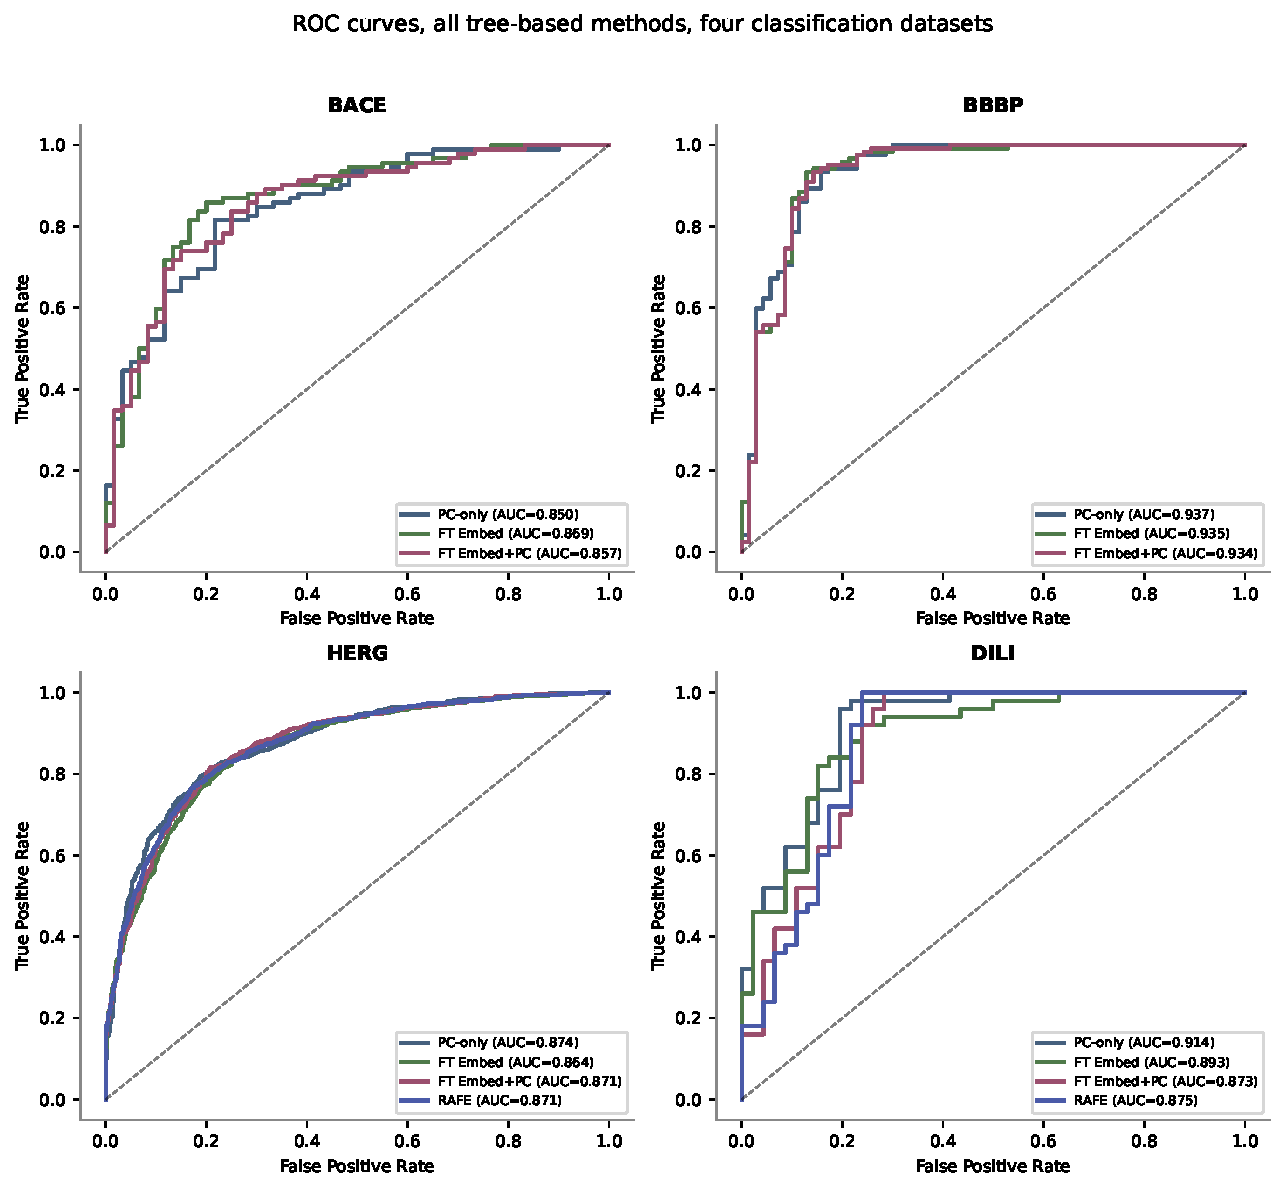
\includegraphics[width=0.95\textwidth]{roc_curves_4datasets.pdf}
  \caption{ROC curves for best configuration of tree-based methods (PC-only, FT Embed, FT Embed+PC and RAFE), on all four binary classification datasets in this study: two MoleculeNet (BACE, BBBP) and two TDC ADMET tasks (hERG, DILI).}
  \label{fig:roc_4ds}
\end{figure*}

\begin{figure*}[!ht]
  \centering
  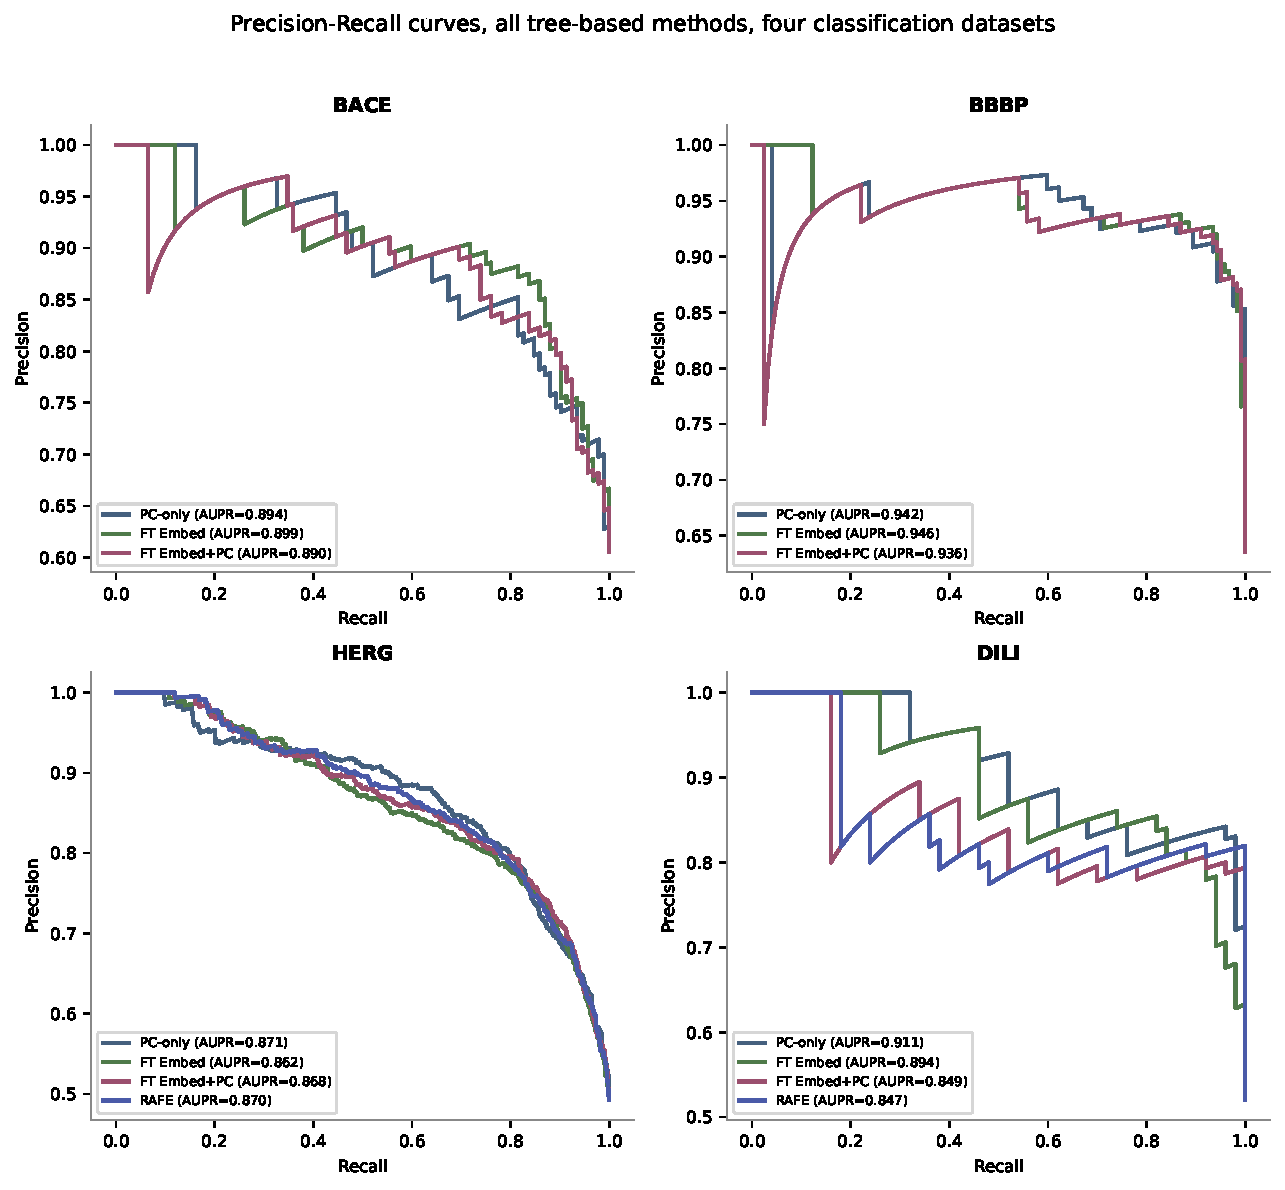
\includegraphics[width=0.95\textwidth]{pr_curves_4datasets.pdf}
  \caption{Precision-recall curves for the same models and datasets as Figure~\ref{fig:roc_4ds}. DILI's small test set ($n=96$) produces visibly noisier curves than the other three datasets, consistent with its wide bootstrapped SE throughout this paper.}
  \label{fig:pr_4ds}
\end{figure*}

\paragraph{Caco-2 Permeability (Regression).} Table~\ref{tab:caco2} shows the Caco-2 results (single runs), ranked by Spearman correlation. PC-only has the highest value (Spearman$=0.853$, R\textsuperscript{2}$=0.744$, SE$=0.021$), ahead of RAFE (ChemBERTa-MTR~$+$~CatBoost, Spearman$=0.835$, R\textsuperscript{2}$=0.663$, SE$=0.026$) and FT~Embed+PC (Spearman$=0.824$, R\textsuperscript{2}$=0.672$). Five-seed means tell the same story: $\mCACORAFE$ for RAFE, $\mCACOFTPC$ for FT Embed+PC, $\mCACOFT$ for FT Embed and $\mCACOPC$ for PC-only. The clear effect on Caco-2 is the gain of RAFE and of FT Embed+PC over the fine-tuned embedding alone ($+0.084$ for LightGBM; 95\% interval $+0.059$ to $+0.111$, Table~\ref{tab:full_caco2}). Most of that gain is already provided by the descriptors, which are mechanistically close to membrane permeability, and a descriptor-only model matches or exceeds every CLM-based stage. The full set of ablation results is in Supplementary Table~S7.

\begin{table*}[!ht]
\centering
\caption{Best configurations on Caco-2 permeability (regression, TDC ADMET Group), ranked by Spearman.}
\label{tab:caco2}
\resizebox{0.95\textwidth}{!}{
\begin{tabular}{lllrrrr}
\toprule
Modality & CLM & ML & R\textsuperscript{2} & MAE & Spearman & SE(Spearman) \\
\midrule
PC-only$^*$ & --- & CatBoost & 0.744 & 0.273 & \textbf{0.853} & \textbf{0.0211} \\
Chemprop    & --- & --- & 0.534 & 0.359 & 0.802 & 0.0294 \\
GCN         & --- & --- & 0.244 & 0.491 & 0.733 & 0.0342 \\
\midrule
E2E LoRA    & ChemBERTa-MTR & --- & 0.622 & 0.340 & 0.789 & 0.0318 \\
E2E LoRA    & Uni-Mol       & --- & 0.411 & 0.432 & 0.580 & 0.0565 \\
\midrule
FT Embed    & ChemBERTa-MTR & CatBoost & \textbf{0.668} & 0.318 & 0.821 & 0.0284 \\
FT Embed+PC & ChemBERTa-MTR & LightGBM & 0.672 & \textbf{0.308} & 0.824 & 0.0277 \\
RAFE        & ChemBERTa-MTR & CatBoost & 0.663 & 0.324 & 0.835 & 0.0256 \\
\bottomrule
\end{tabular}
}
\end{table*}

\paragraph{Half-Life (Regression).} Table~\ref{tab:half_life} reports Half-Life results (single runs), ranked by Spearman correlation. FT Embed (MolFormer-XL~$+$~XGBoost) has the highest value (Spearman$=0.600$, R\textsuperscript{2}$=0.083$, SE$=0.056$), ahead of FT~Embed+PC (Spearman$=0.593$) and PC-only (Spearman$=0.502$, SE$=0.075$). Half-Life is the noisiest dataset ($n_\text{test}=133$, R\textsuperscript{2} $< 0.11$ for every method after log1p transformation and outlier removal), and the bands of FT Embed and PC-only overlap. RAFE is not favorable here: with LightGBM it is below FT Embed+PC ($-0.023$, 95\% interval $-0.044$ to $-0.002$). Spearman and R\textsuperscript{2} behave differently on this dataset, as discussed in Section~\ref{sec:metrics}. The full per-embedding, per-loss ablation is in Supplementary Table~S8.

\begin{table*}[!ht]
\centering
\caption{Best configurations on drug Half-Life (regression, TDC ADMET Group, log1p target), ranked by Spearman.}
\label{tab:half_life}
\resizebox{0.95\textwidth}{!}{
\begin{tabular}{lllrrrr}
\toprule
Modality & CLM & ML & R\textsuperscript{2} & MAE (h) & Spearman & SE(Spearman) \\
\midrule
PC-only     & --- & XGBoost & 0.110 & 5.687 & 0.502 & 0.0750 \\
Chemprop    & --- & --- & -0.020 & 6.325 & 0.332 & 0.0841 \\
GCN         & --- & --- & 0.114 & 5.928 & 0.418 & 0.0777 \\
\midrule
E2E LoRA    & ChemBERTa-MTR & --- & 0.072 & 6.367 & 0.541 & 0.0654 \\
E2E LoRA    & Uni-Mol       & --- & -0.072 & 6.937 & 0.518 & 0.0720 \\
\midrule
FT Embed$^*$& MolFormer-XL & XGBoost & \textbf{0.083} & \textbf{5.639} & \textbf{0.600} & \textbf{0.0562} \\
FT Embed+PC & MolFormer-XL & XGBoost & 0.090 & 5.594 & 0.593 & 0.0535 \\
RAFE        & MolFormer-XL & XGBoost & 0.090 & 5.557 & 0.568 & 0.0579 \\
\bottomrule
\end{tabular}
}
\end{table*}

\subsection{Controlled Comparison of Representations}\label{sec:controlled}
The single-run tables compare the best row of each mode, and these rows can come from different tree models. To separate the effect of the representation from that of the tree, we ran PC-only, FT Embed, FT Embed+PC and RAFE with the same code, splits, test molecules, tuning budget, three tree models and five seeds, for one embedding configuration per dataset (two for BACE; Table~\ref{tab:controlled}, Figure~\ref{fig:matrix}).

Three results follow. First, RAFE is never significantly better or worse than FT Embed+PC: none of the 24 paired comparisons (eight dataset configurations, three trees) has an interval that excludes zero. Second, RAFE is significantly better than FT Embed alone in 5 of 24 comparisons (Caco-2 with all three trees, DILI with XGBoost and hERG with LightGBM) and never worse. Third, RAFE is significantly below PC-only in 4 of 24 comparisons (hERG with all three trees, Flavor with XGBoost) and never significantly above it. The point estimates favor the fine-tuned stages over PC-only on BACE (MolFormer), BBBP and Half-Life, whereas PC-only is highest or tied on Caco-2, hERG and Flavor; none of the former differences is significant.

Across the matched embedding-loss-tree configurations of the supplementary tables, RAFE exceeds FT Embed on four of seven datasets (BBBP $+0.014$, Wilcoxon $p=0.025$; hERG $+0.006$, $p=0.015$; DILI $+0.052$, $p=0.012$; Caco-2 $+0.085$, $p<0.001$; Figure~\ref{fig:ladder}). These tests are descriptive, because the configurations share one test set.

\begin{table*}[!ht]
\centering
\caption{Controlled comparison: mean test metric over five seeds for each representation, tree model and dataset (one embedding configuration per dataset; MCC for classification, Spearman for regression). Every row uses identical splits, test molecules and tuning budget.}
\label{tab:controlled}
\footnotesize
\begin{tabular}{lllllll}
\toprule
Dataset (embedding) & Metric & Tree & PC-only & FT Embed & FT Embed+PC & RAFE \\
\midrule
BACE (MolFormer-WL) & MCC & CatBoost & 0.465 & \textbf{0.546} & 0.528 & 0.518 \\
BACE (MolFormer-WL) & MCC & LightGBM & 0.485 & 0.539 & 0.549 & \textbf{0.553} \\
BACE (MolFormer-WL) & MCC & XGBoost & 0.477 & \textbf{0.542} & 0.538 & 0.527 \\
BACE (Uni-Mol-WL) & MCC & CatBoost & \textbf{0.465} & 0.390 & 0.440 & 0.425 \\
BACE (Uni-Mol-WL) & MCC & LightGBM & \textbf{0.485} & 0.421 & 0.439 & 0.424 \\
BACE (Uni-Mol-WL) & MCC & XGBoost & \textbf{0.477} & 0.429 & 0.440 & 0.419 \\
BBBP (MolFormer-FL) & MCC & CatBoost & 0.726 & 0.762 & 0.768 & \textbf{0.799} \\
BBBP (MolFormer-FL) & MCC & LightGBM & 0.733 & \textbf{0.768} & 0.755 & 0.767 \\
BBBP (MolFormer-FL) & MCC & XGBoost & 0.731 & 0.783 & \textbf{0.785} & 0.779 \\
Caco-2 (ChemBERTa-MTR) & Spearman & CatBoost & \textbf{0.840} & 0.809 & 0.833 & 0.833 \\
Caco-2 (ChemBERTa-MTR) & Spearman & LightGBM & \textbf{0.834} & 0.789 & 0.819 & 0.816 \\
Caco-2 (ChemBERTa-MTR) & Spearman & XGBoost & \textbf{0.833} & 0.788 & 0.813 & 0.817 \\
DILI (Uni-Mol-FL) & MCC & CatBoost & 0.638 & 0.595 & \textbf{0.683} & 0.669 \\
DILI (Uni-Mol-FL) & MCC & LightGBM & 0.654 & 0.574 & \textbf{0.690} & 0.658 \\
DILI (Uni-Mol-FL) & MCC & XGBoost & 0.672 & 0.520 & 0.693 & \textbf{0.697} \\
Flavor (MolFormer-WL) & MCC & CatBoost & \textbf{0.798} & 0.789 & 0.789 & 0.786 \\
Flavor (MolFormer-WL) & MCC & LightGBM & \textbf{0.798} & 0.779 & 0.783 & 0.785 \\
Flavor (MolFormer-WL) & MCC & XGBoost & \textbf{0.809} & 0.782 & 0.780 & 0.782 \\
Half-Life (MolFormer) & Spearman & CatBoost & 0.530 & \textbf{0.604} & 0.596 & 0.577 \\
Half-Life (MolFormer) & Spearman & LightGBM & 0.477 & 0.550 & \textbf{0.558} & 0.512 \\
Half-Life (MolFormer) & Spearman & XGBoost & 0.499 & 0.592 & \textbf{0.595} & 0.559 \\
hERG (MolFormer-FL) & MCC & CatBoost & \textbf{0.593} & 0.536 & 0.543 & 0.537 \\
hERG (MolFormer-FL) & MCC & LightGBM & \textbf{0.577} & 0.532 & 0.545 & 0.544 \\
hERG (MolFormer-FL) & MCC & XGBoost & \textbf{0.594} & 0.545 & 0.546 & 0.545 \\
\bottomrule
\end{tabular}

\end{table*}

\begin{figure}[!ht]
  \centering
  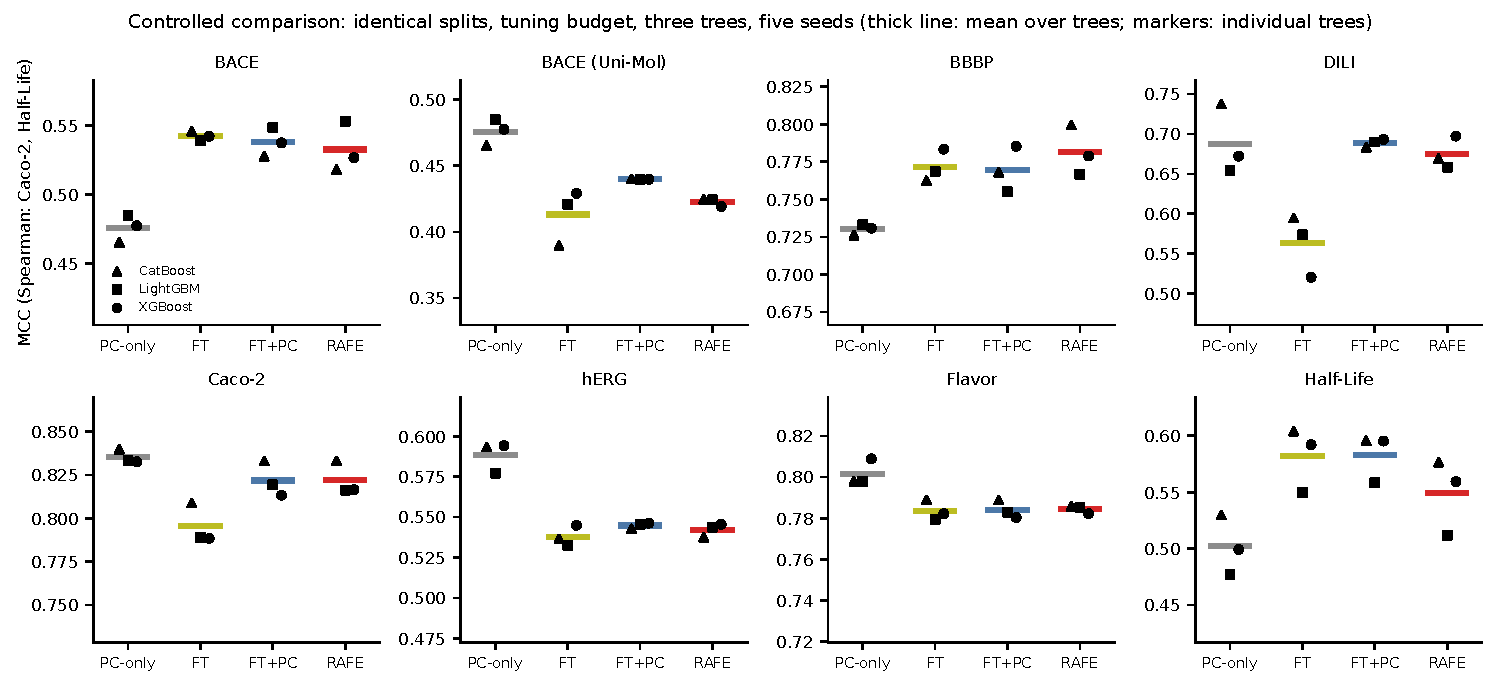
\includegraphics[width=0.99\textwidth]{controlled_matrix_v3.pdf}
  \caption{The controlled comparison of Table~\ref{tab:controlled}. The thick line is the mean over trees and the markers are individual trees.}
  \label{fig:matrix}
\end{figure}

\begin{figure}[!ht]
  \centering
  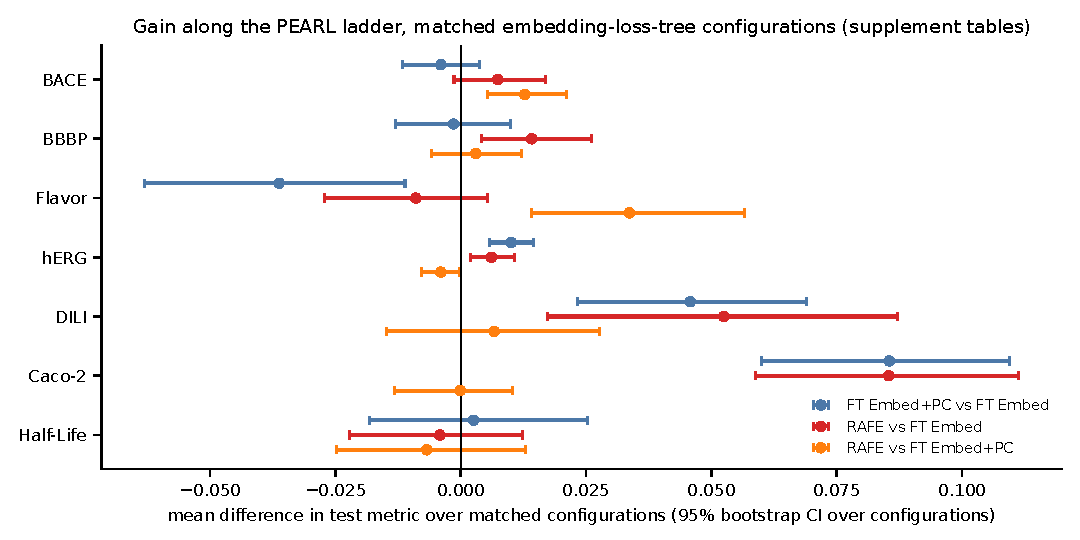
\includegraphics[width=0.99\textwidth]{ladder_gain_v3.pdf}
  \caption{Difference between pipeline stages over matched embedding-loss-tree configurations (supplementary tables). Intervals are bootstrap intervals over configurations and are descriptive, because configurations share a test set.}
  \label{fig:ladder}
\end{figure}

\paragraph{Full same-tree tables.} Table~\ref{tab:controlled} uses one embedding per dataset. Tables~\ref{tab:full_dili}, \ref{tab:full_caco2} and~\ref{tab:full_bbbp} extend the comparison to the full grid for the datasets on which RAFE is most often discussed: every embedding and loss combination, with the three stages compared inside one tree. The bottom rows give the difference pooled over rows and seeds with a paired interval. On DILI, RAFE exceeds FT Embed with both trees (XGBoost $+0.072$, 95\% interval $+0.036$ to $+0.111$; LightGBM $+0.039$, $+0.002$ to $+0.076$). Against FT Embed+PC the result depends on the tree: with XGBoost the pooled difference is $+0.032$ ($+0.005$ to $+0.060$), and with LightGBM it is $-0.009$ ($-0.029$ to $+0.012$). On Caco-2, RAFE and FT Embed+PC are indistinguishable and both exceed FT Embed (LightGBM: $+0.084$, $+0.059$ to $+0.111$), while PC-only exceeds every CLM-based stage. On BBBP, no stage separates from another with either tree. \pending{CatBoost columns of the full tables, which are still running}

\begin{table*}[!ht]
\centering
\caption{DILI, full same-tree comparison. Mean $\pm$ SD of the test MCC over five seeds for each embedding and loss combination. Bold: best of the three stages within the row and tree. The last two rows give the difference pooled over rows and seeds with a paired bootstrap interval.}
\label{tab:full_dili}
\scriptsize
\begin{tabular}{@{}lcccccc@{}}
\toprule
 & \multicolumn{3}{c}{XGBoost} & \multicolumn{3}{c}{LightGBM} \\
\cmidrule(lr){2-4} \cmidrule(lr){5-7}
Embedding, loss & FT Embed & FT Embed+PC & RAFE & FT Embed & FT Embed+PC & RAFE \\
\midrule
ChemBERTa-MLM FL & 0.536 $\pm$ 0.025 & 0.522 $\pm$ 0.020 & \textbf{0.637 $\pm$ 0.024} & 0.613 $\pm$ 0.047 & \textbf{0.645 $\pm$ 0.039} & 0.617 $\pm$ 0.060 \\
ChemBERTa-MLM WL & 0.563 $\pm$ 0.059 & 0.542 $\pm$ 0.057 & \textbf{0.565 $\pm$ 0.024} & \textbf{0.579 $\pm$ 0.021} & 0.574 $\pm$ 0.030 & 0.564 $\pm$ 0.021 \\
ChemBERTa-MTR FL & 0.412 $\pm$ 0.046 & 0.467 $\pm$ 0.030 & \textbf{0.543 $\pm$ 0.040} & 0.416 $\pm$ 0.021 & 0.521 $\pm$ 0.025 & \textbf{0.535 $\pm$ 0.052} \\
ChemBERTa-MTR WL & 0.546 $\pm$ 0.026 & 0.542 $\pm$ 0.028 & \textbf{0.562 $\pm$ 0.025} & \textbf{0.558 $\pm$ 0.017} & 0.534 $\pm$ 0.025 & 0.538 $\pm$ 0.031 \\
MolFormer FL & 0.507 $\pm$ 0.038 & 0.537 $\pm$ 0.018 & \textbf{0.541 $\pm$ 0.021} & 0.545 $\pm$ 0.018 & 0.553 $\pm$ 0.031 & \textbf{0.608 $\pm$ 0.023} \\
MolFormer WL & 0.446 $\pm$ 0.032 & \textbf{0.472 $\pm$ 0.019} & 0.461 $\pm$ 0.027 & 0.491 $\pm$ 0.024 & \textbf{0.517 $\pm$ 0.018} & 0.461 $\pm$ 0.037 \\
Uni-Mol FL & 0.520 $\pm$ 0.075 & 0.693 $\pm$ 0.019 & \textbf{0.697 $\pm$ 0.008} & 0.574 $\pm$ 0.061 & \textbf{0.690 $\pm$ 0.032} & 0.658 $\pm$ 0.039 \\
Uni-Mol WL & 0.576 $\pm$ 0.012 & 0.653 $\pm$ 0.027 & \textbf{0.677 $\pm$ 0.013} & 0.554 $\pm$ 0.035 & \textbf{0.675 $\pm$ 0.008} & 0.658 $\pm$ 0.024 \\
\midrule
PC-only (473 descriptors) & 0.672 $\pm$ 0.034 &  &  & 0.654 $\pm$ 0.015 &  &  \\
RAFE $-$ FT Embed [95\% CI] & \multicolumn{3}{c}{+0.072 [+0.036, +0.111]} & \multicolumn{3}{c}{+0.039 [+0.002, +0.076]} \\
RAFE $-$ FT Embed+PC [95\% CI] & \multicolumn{3}{c}{+0.032 [+0.005, +0.060]} & \multicolumn{3}{c}{$-$0.009 [$-$0.029, +0.012]} \\
\bottomrule
\end{tabular}

\end{table*}

\begin{table*}[!ht]
\centering
\caption{Caco-2, full same-tree comparison (test Spearman, mean $\pm$ SD over five seeds; layout as in Table~\ref{tab:full_dili}).}
\label{tab:full_caco2}
\scriptsize
\begin{tabular}{@{}lccccccccc@{}}
\toprule
 & \multicolumn{3}{c}{XGBoost} & \multicolumn{3}{c}{LightGBM} & \multicolumn{3}{c}{CatBoost} \\
\cmidrule(lr){2-4} \cmidrule(lr){5-7} \cmidrule(lr){8-10}
Embedding, loss & FT Embed & FT Embed+PC & RAFE & FT Embed & FT Embed+PC & RAFE & FT Embed & FT Embed+PC & RAFE \\
\midrule
ChemBERTa-MLM Huber & 0.683 $\pm$ 0.010 & \textbf{0.750 $\pm$ 0.009} & 0.734 $\pm$ 0.005 & 0.671 $\pm$ 0.009 & \textbf{0.738 $\pm$ 0.012} & 0.711 $\pm$ 0.013 & 0.671 $\pm$ 0.006 & \textbf{0.748 $\pm$ 0.012} & 0.745 $\pm$ 0.018 \\
ChemBERTa-MTR Huber & 0.788 $\pm$ 0.005 & 0.813 $\pm$ 0.007 & \textbf{0.817 $\pm$ 0.007} & 0.789 $\pm$ 0.003 & \textbf{0.819 $\pm$ 0.006} & 0.816 $\pm$ 0.005 & 0.809 $\pm$ 0.008 & \textbf{0.833 $\pm$ 0.005} & 0.833 $\pm$ 0.005 \\
MolFormer Huber & 0.592 $\pm$ 0.028 & 0.712 $\pm$ 0.013 & \textbf{0.717 $\pm$ 0.016} & 0.655 $\pm$ 0.021 & 0.743 $\pm$ 0.014 & \textbf{0.748 $\pm$ 0.005} & 0.633 $\pm$ 0.015 & \textbf{0.753 $\pm$ 0.018} & 0.748 $\pm$ 0.014 \\
Uni-Mol Huber & 0.653 $\pm$ 0.013 & 0.769 $\pm$ 0.009 & \textbf{0.774 $\pm$ 0.005} & 0.586 $\pm$ 0.017 & 0.758 $\pm$ 0.003 & \textbf{0.761 $\pm$ 0.011} & 0.687 $\pm$ 0.023 & \textbf{0.811 $\pm$ 0.010} & 0.800 $\pm$ 0.012 \\
\midrule
PC-only (473 descriptors) & 0.833 $\pm$ 0.004 &  &  & 0.834 $\pm$ 0.006 &  &  & 0.840 $\pm$ 0.007 &  &  \\
RAFE $-$ FT Embed [95\% CI] & \multicolumn{3}{c}{+0.082 [+0.056, +0.108]} & \multicolumn{3}{c}{+0.084 [+0.059, +0.111]} & \multicolumn{3}{c}{+0.082 [+0.057, +0.107]} \\
RAFE $-$ FT Embed+PC [95\% CI] & \multicolumn{3}{c}{$-$0.000 [$-$0.006, +0.006]} & \multicolumn{3}{c}{$-$0.005 [$-$0.011, +0.001]} & \multicolumn{3}{c}{$-$0.005 [$-$0.009, $-$0.001]} \\
\bottomrule
\end{tabular}

\end{table*}

\begin{table*}[!ht]
\centering
\caption{BBBP, full same-tree comparison (test MCC, mean $\pm$ SD over five seeds; layout as in Table~\ref{tab:full_dili}).}
\label{tab:full_bbbp}
\scriptsize
\begin{tabular}{@{}lcccccc@{}}
\toprule
 & \multicolumn{3}{c}{XGBoost} & \multicolumn{3}{c}{LightGBM} \\
\cmidrule(lr){2-4} \cmidrule(lr){5-7}
Embedding, loss & FT Embed & FT Embed+PC & RAFE & FT Embed & FT Embed+PC & RAFE \\
\midrule
ChemBERTa-MLM FL & 0.732 $\pm$ 0.009 & \textbf{0.746 $\pm$ 0.013} & 0.733 $\pm$ 0.006 & 0.741 $\pm$ 0.012 & \textbf{0.751 $\pm$ 0.009} & 0.737 $\pm$ 0.007 \\
ChemBERTa-MLM WL & \textbf{0.711 $\pm$ 0.006} & 0.707 $\pm$ 0.013 & 0.705 $\pm$ 0.001 & 0.700 $\pm$ 0.031 & 0.698 $\pm$ 0.017 & \textbf{0.703 $\pm$ 0.011} \\
ChemBERTa-MTR FL & 0.683 $\pm$ 0.013 & \textbf{0.690 $\pm$ 0.005} & 0.659 $\pm$ 0.005 & \textbf{0.675 $\pm$ 0.006} & 0.671 $\pm$ 0.010 & 0.673 $\pm$ 0.011 \\
ChemBERTa-MTR WL & 0.701 $\pm$ 0.005 & 0.703 $\pm$ 0.012 & \textbf{0.708 $\pm$ 0.010} & \textbf{0.696 $\pm$ 0.006} & 0.676 $\pm$ 0.013 & 0.687 $\pm$ 0.007 \\
MolFormer FL & 0.783 $\pm$ 0.010 & \textbf{0.785 $\pm$ 0.016} & 0.779 $\pm$ 0.010 & \textbf{0.769 $\pm$ 0.026} & 0.755 $\pm$ 0.015 & 0.767 $\pm$ 0.015 \\
MolFormer WL & 0.730 $\pm$ 0.014 & \textbf{0.737 $\pm$ 0.008} & 0.732 $\pm$ 0.006 & 0.752 $\pm$ 0.014 & \textbf{0.761 $\pm$ 0.012} & 0.746 $\pm$ 0.013 \\
Uni-Mol FL & 0.721 $\pm$ 0.017 & 0.734 $\pm$ 0.021 & \textbf{0.735 $\pm$ 0.031} & 0.731 $\pm$ 0.017 & 0.742 $\pm$ 0.024 & \textbf{0.745 $\pm$ 0.011} \\
Uni-Mol WL & 0.701 $\pm$ 0.016 & 0.729 $\pm$ 0.022 & \textbf{0.735 $\pm$ 0.012} & 0.713 $\pm$ 0.023 & \textbf{0.743 $\pm$ 0.012} & 0.728 $\pm$ 0.029 \\
\midrule
PC-only (473 descriptors) & 0.731 $\pm$ 0.033 &  &  & 0.733 $\pm$ 0.030 &  &  \\
RAFE $-$ FT Embed [95\% CI] & \multicolumn{3}{c}{+0.003 [$-$0.007, +0.012]} & \multicolumn{3}{c}{+0.001 [$-$0.012, +0.013]} \\
RAFE $-$ FT Embed+PC [95\% CI] & \multicolumn{3}{c}{$-$0.006 [$-$0.014, +0.003]} & \multicolumn{3}{c}{$-$0.002 [$-$0.009, +0.005]} \\
\bottomrule
\end{tabular}

\end{table*}

\subsection{Best Configuration per Dataset on Five-Seed Means}\label{sec:best_configs}
PEARL is a configuration benchmark: for each dataset the question is which embedding, loss, tree and stage works best. Because the best of many configurations is optimistic when taken from one run, we repeated the full configuration grid with five seeds for XGBoost and LightGBM on five datasets (BACE, BBBP, DILI, Caco-2, Half-Life; Figure~\ref{fig:grid}). Table~\ref{tab:best_configs} lists the best configuration of each stage by five-seed test mean, the single-run value of the same modality in the original tables, and the paired difference to the runner-up. \pending{CatBoost for the five datasets, and hERG and Flavor}

Three observations follow. The best configuration is MolFormer in \nmf{} of \nrows{} rows, and the single-run values of the original tables exceed the five-seed means in \nsr{} of \nrows{} rows; the largest drop is for DILI RAFE, from 0.790 to \mDILIRAFE{}. The best configuration is separable from the runner-up in only \nsep{} of \nrows{} rows, so the identity of the best configuration is itself uncertain and claims should rest on paired differences. Selecting the configuration by training-split cross-validation is unreliable on these scaffold splits: it lowers the RAFE score by \gaplo{} to \gaphi{} (MCC or Spearman) relative to the test-based choice, and we do not use it for ranking.

Ranking the best configuration of each of seven methods on the \nds{} datasets completed so far, RAFE is in the top three on \ntop{} of \nds{} (mean rank \mrankRAFE{}). FT Embed+PC has mean rank \mrankFTPC{}, FT Embed \mrankFT{} and PC-only \mrankPC{}. The single-run best values of the original tables give a more favorable picture for RAFE: it is first on BBBP and DILI and in the top three on \srtop{} of seven datasets (Figure~\ref{fig:ranking}). If each method is instead represented by the median of its configurations, RAFE is in the top three on \medtop{} datasets (mean rank \medmean{}), and PC-only has a mean rank of \medpc{}. We read these results as showing that RAFE is a consistently competitive final stage, and not a general winner. \pending{ranking including hERG and Flavor}

\begin{table*}[!ht]
\centering
\caption{Best configuration per dataset and stage, judged on five-seed test means (XGBoost and LightGBM). ``Single run'' is the best value of the same modality in the original tables. The last column is the difference between the best and the runner-up configuration with a paired 95\% bootstrap interval.}
\label{tab:best_configs}
\scriptsize
\adjustbox{max width=\textwidth}{\begin{tabular}{lllllll}
\toprule
Dataset & Stage & Best configuration (embedding, loss / tree) & Test, 5-seed mean $\pm$ SD & Single run in the original tables & Runner-up (test mean) & Best minus runner-up [95\% CI] \\
\midrule
BACE & FT Embed & MolFormer FL / CatBoost & 0.549 $\pm$ 0.016 & 0.557 & MolFormer WL / CatBoost (0.546) & +0.003 [$-$0.066, +0.070] \\
BACE & FT Embed+PC & MolFormer FL / CatBoost & 0.556 $\pm$ 0.014 & 0.550 & MolFormer WL / LightGBM (0.549) & +0.008 [$-$0.064, +0.077] \\
BACE & RAFE & MolFormer WL / LightGBM & 0.553 $\pm$ 0.017 & 0.561 & MolFormer FL / CatBoost (0.551) & +0.002 [$-$0.066, +0.073] \\
BBBP & FT Embed & MolFormer FL / XGBoost & 0.783 $\pm$ 0.010 & 0.787 & MolFormer FL / LightGBM (0.768) & +0.015 [$-$0.014, +0.048] \\
BBBP & FT Embed+PC & MolFormer FL / XGBoost & 0.785 $\pm$ 0.016 & 0.789 & MolFormer FL / CatBoost (0.768) & +0.017 [$-$0.024, +0.061] \\
BBBP & RAFE & MolFormer FL / XGBoost & 0.779 $\pm$ 0.009 & 0.798 & MolFormer WL / CatBoost (0.771) & +0.008 [$-$0.054, +0.072] \\
Caco-2 & FT Embed & ChemBERTa-MTR Huber / CatBoost & 0.809 $\pm$ 0.008 & 0.821 & ChemBERTa-MTR Huber / LightGBM (0.789) & \textbf{+0.020 [+0.002, +0.038]} \\
Caco-2 & FT Embed+PC & ChemBERTa-MTR Huber / CatBoost & 0.833 $\pm$ 0.005 & 0.827 & ChemBERTa-MTR Huber / LightGBM (0.819) & +0.014 [$-$0.004, +0.033] \\
Caco-2 & RAFE & ChemBERTa-MTR Huber / CatBoost & 0.833 $\pm$ 0.005 & 0.835 & ChemBERTa-MTR Huber / XGBoost (0.817) & +0.017 [$-$0.004, +0.038] \\
DILI & FT Embed & Uni-Mol WL / CatBoost & 0.630 $\pm$ 0.026 & 0.673 & ChemBERTa-MLM WL / CatBoost (0.628) & +0.002 [$-$0.171, +0.180] \\
DILI & FT Embed+PC & Uni-Mol FL / XGBoost & 0.693 $\pm$ 0.019 & 0.703 & Uni-Mol FL / LightGBM (0.690) & +0.003 [$-$0.044, +0.047] \\
DILI & RAFE & Uni-Mol FL / XGBoost & 0.697 $\pm$ 0.008 & 0.790 & Uni-Mol WL / XGBoost (0.677) & +0.020 [$-$0.050, +0.097] \\
Flavor & FT Embed & MolFormer WL / CatBoost & 0.789 $\pm$ 0.004 & 0.793 & ChemBERTa-MTR FL / CatBoost (0.787) & +0.002 [$-$0.016, +0.019] \\
Flavor & FT Embed+PC & Uni-Mol FL / XGBoost & 0.791 $\pm$ 0.004 & 0.801 & MolFormer WL / CatBoost (0.789) & +0.002 [$-$0.014, +0.018] \\
Flavor & RAFE & Uni-Mol FL / XGBoost & 0.796 $\pm$ 0.010 & 0.804 & Uni-Mol WL / XGBoost (0.790) & +0.006 [$-$0.002, +0.014] \\
Half-Life & FT Embed & MolFormer Huber / CatBoost & 0.604 $\pm$ 0.024 & 0.623 & MolFormer Huber / XGBoost (0.592) & +0.012 [$-$0.037, +0.061] \\
Half-Life & FT Embed+PC & MolFormer Huber / CatBoost & 0.596 $\pm$ 0.027 & 0.593 & MolFormer Huber / XGBoost (0.595) & +0.000 [$-$0.054, +0.055] \\
Half-Life & RAFE & MolFormer Huber / CatBoost & 0.577 $\pm$ 0.018 & 0.568 & MolFormer Huber / XGBoost (0.559) & +0.017 [$-$0.036, +0.066] \\
hERG & FT Embed & MolFormer WL / LightGBM & 0.574 $\pm$ 0.005 & 0.580 & MolFormer WL / XGBoost (0.570) & +0.005 [$-$0.002, +0.011] \\
hERG & FT Embed+PC & Uni-Mol FL / LightGBM & 0.591 $\pm$ 0.007 & 0.602 & Uni-Mol FL / CatBoost (0.589) & +0.002 [$-$0.011, +0.015] \\
hERG & RAFE & Uni-Mol FL / LightGBM & 0.589 $\pm$ 0.010 & 0.589 & Uni-Mol FL / CatBoost (0.585) & +0.004 [$-$0.009, +0.016] \\
\bottomrule
\end{tabular}
}
\end{table*}

\begin{figure}[!ht]
  \centering
  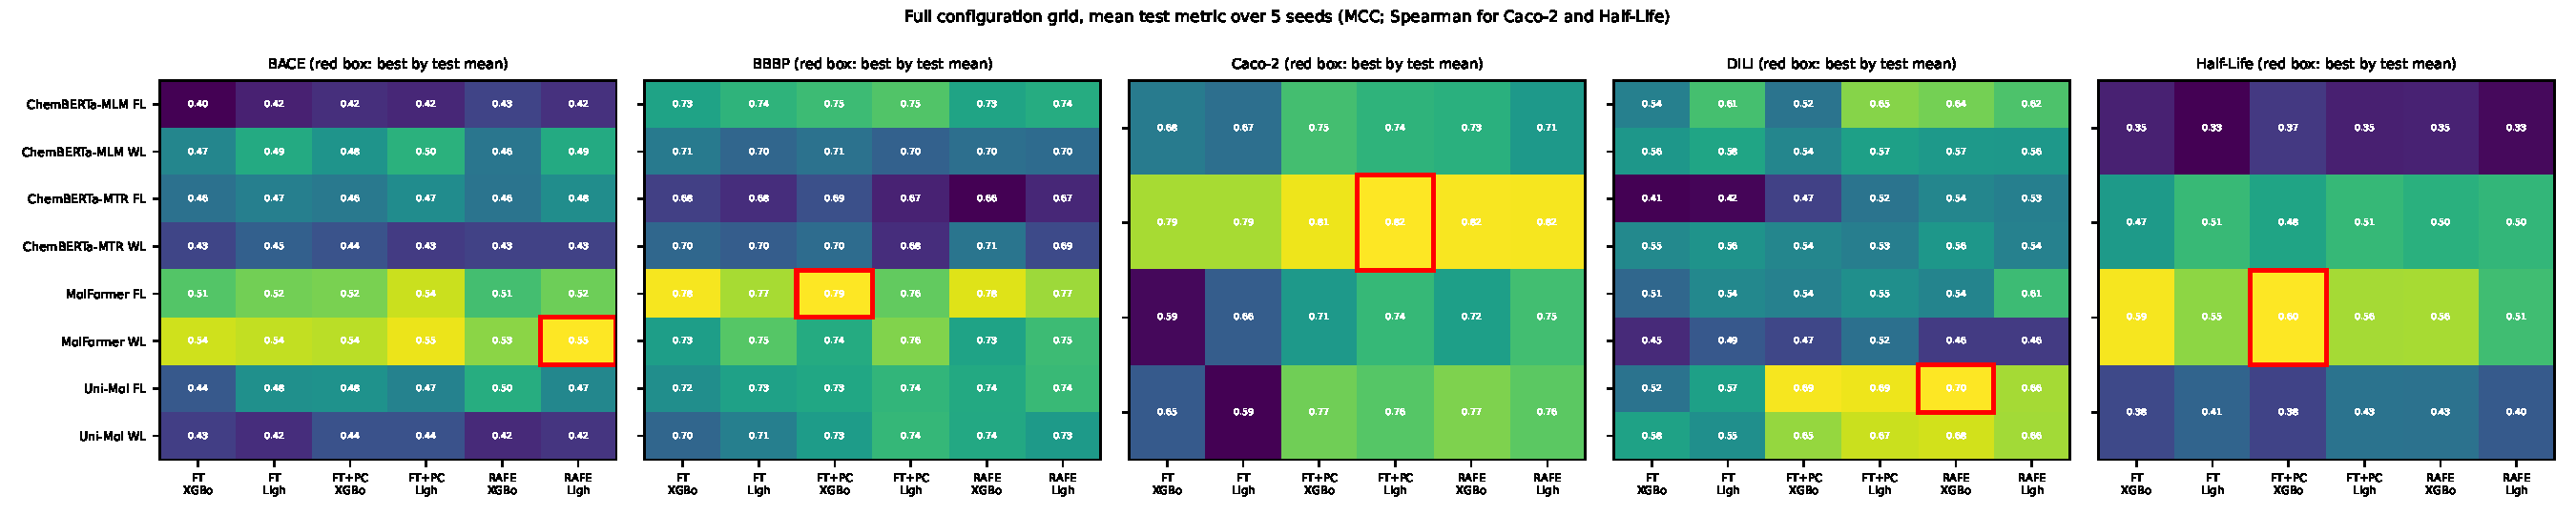
\includegraphics[width=0.99\textwidth]{grid_heatmap_v3.pdf}
  \caption{Five-seed mean test metric over the full configuration grid for the five completed datasets. The red box marks the best cell.}
  \label{fig:grid}
\end{figure}

\begin{figure}[!ht]
  \centering
  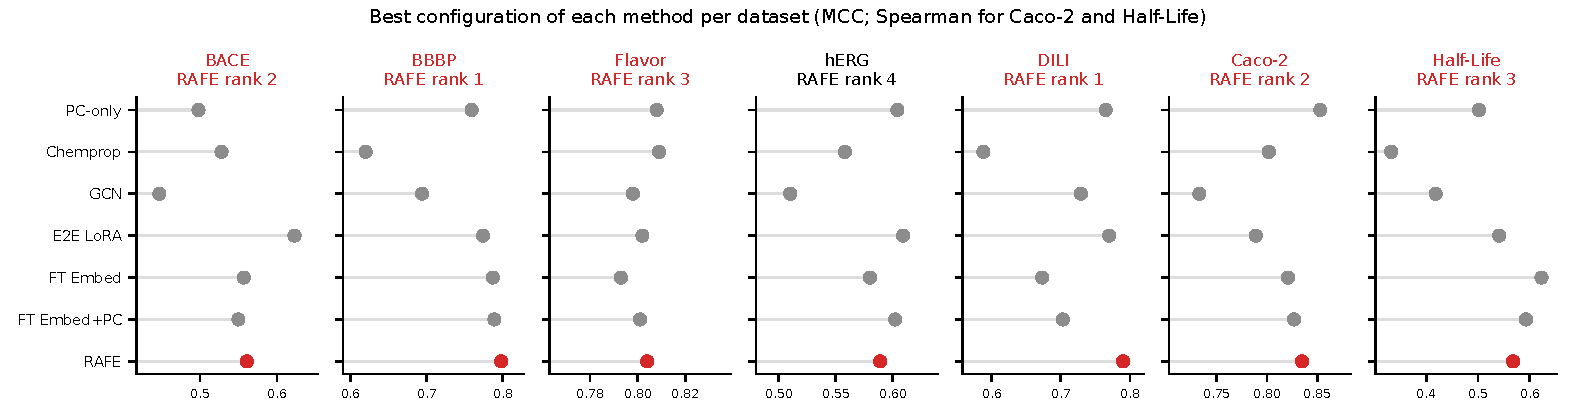
\includegraphics[width=0.8\textwidth]{best_config_ranking_v3.pdf}
  \caption{Best single-run configuration of each method per dataset (red: RAFE).}
  \label{fig:ranking}
\end{figure}

\begin{figure}[!ht]
  \centering
  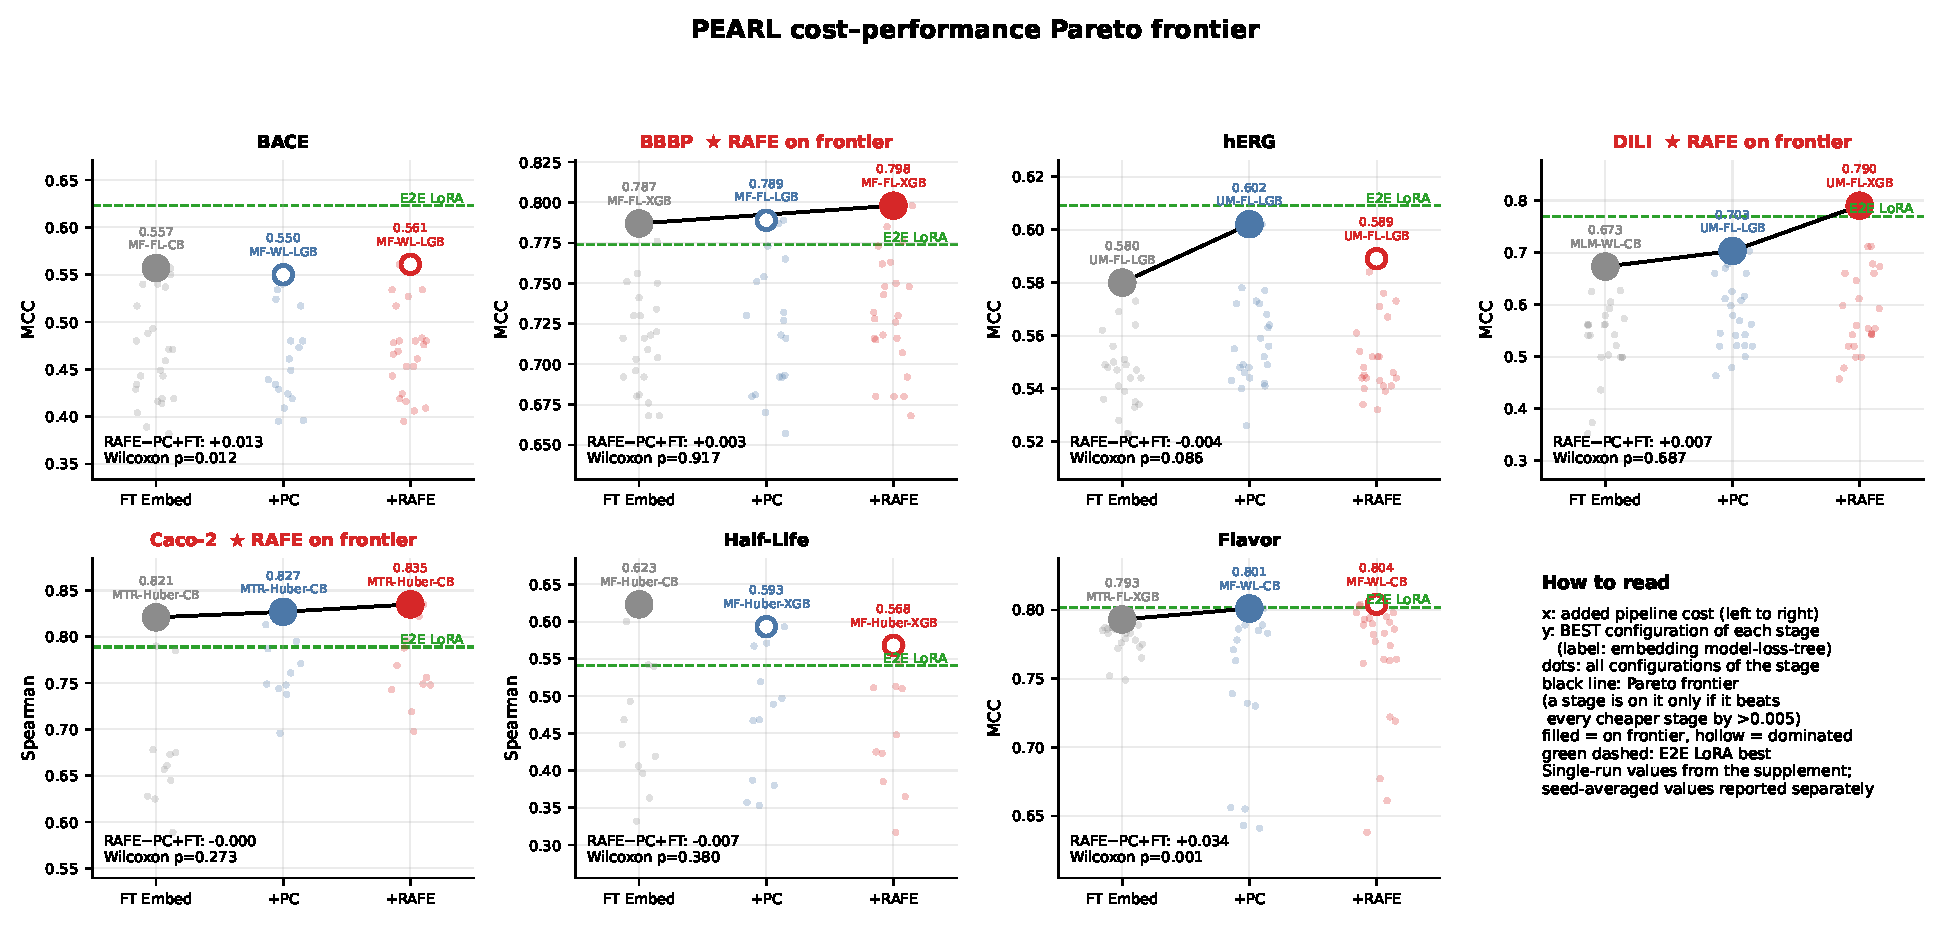
\includegraphics[width=0.8\textwidth]{pareto_frontier_v3.pdf}
  \caption{Cost-performance view of the best configuration of each stage.}
  \label{fig:pareto}
\end{figure}

\subsection{Conventional Fingerprints and Descriptors}\label{sec:fingerprints}
Table~\ref{tab:fingerprints} evaluates ECFP4, ECFP6, MACCS, ECFP4$+$MACCS, the RDKit descriptors and the 473 physicochemical descriptors with the same trees and tuning (best tree shown). Fingerprints alone are clearly weaker than descriptors on Caco-2 (\ecfpcaco{} for ECFP4 versus \pccaco{}), DILI and Half-Life, and comparable on BACE, hERG and Flavor. RAFE is clearly better than ECFP4 alone on DILI ($+\draferecfpdili$) and Caco-2 ($+\draferecfpcaco$). Against PC-only the paired intervals include zero on BBBP, DILI and Caco-2, the three datasets compared.

\begin{table}[!ht]
\centering
\caption{Fingerprint and descriptor baselines (best tree per cell; MCC for classification, Spearman for regression). Three seeds on the smaller datasets and one on hERG and Flavor.}
\label{tab:fingerprints}
\scriptsize
\adjustbox{max width=\textwidth}{\begin{tabular}{lllllll}
\toprule
Dataset & ECFP4 & ECFP6 & MACCS & ECFP4+MACCS & RDKit descriptors & 473 physchem (PC-only) \\
\midrule
BACE & 0.515 & 0.473 & 0.505 & \textbf{0.516} & 0.426 & 0.498 \\
BBBP & 0.688 & 0.673 & 0.700 & 0.700 & 0.729 & \textbf{0.748} \\
Flavor & 0.799 & 0.797 & 0.804 & \textbf{0.815} & 0.800 & 0.806 \\
hERG & 0.584 & 0.560 & 0.539 & 0.587 & 0.593 & \textbf{0.601} \\
DILI & 0.546 & 0.486 & 0.612 & 0.607 & 0.731 & \textbf{0.732} \\
Caco-2 & 0.607 & 0.517 & 0.800 & 0.791 & \textbf{0.842} & 0.838 \\
Half-Life & 0.444 & 0.414 & \textbf{0.526} & 0.524 & 0.516 & \textbf{0.526} \\
\bottomrule
\end{tabular}
}
\end{table}

\subsection{What Does RAFE Add?}\label{sec:rafe_effectiveness}
This section addresses H2. We examine which RAFE components matter, how sensitive RAFE is to its retrieval settings, what it adds to the embedding and descriptors, and whether label-free variants change the conclusion.

\paragraph{Feature groups.} Adding or removing any of the four RAFE groups changes the score by no more than 0.02 in \fracsmall\% of the \ncellsabl{} dataset-by-arm cells (Table~\ref{tab:groups}, Figure~\ref{fig:groups}). The \nbig{} larger shifts are all decreases and are confined to \bigcfg{}, which have the smallest test sets in the study. No single group is responsible for the effect of RAFE, which is consistent with the groups carrying overlapping information.

\paragraph{Retrieval metric and neighbor count.} We compared CLM-cosine retrieval with Morgan-Tanimoto retrieval and with random retrieval (five independent random draws), and swept $k$ from 1 to 100. Of \nkcomp{} paired comparisons, \nkexc{} have an interval that excludes zero (\excdetails; Figure~\ref{fig:retrieval}), and both differences are below 0.011 in size. RAFE therefore does not need its retrieval settings tuned. Random neighbors perform as well as similar ones, which shows that RAFE acts as chemical-space context and not as an analogue lookup. \pending{BBBP neighbor-count sweep (cells still running)}

\paragraph{Complementarity with the embedding and descriptors.} The per-molecule gain of RAFE over FT Embed+PC is unrelated to ZINC-250k coverage (Spearman correlation between \spmin{} and \spmax{} across datasets; all intervals include zero; Figure~\ref{fig:e10}, left). A ridge model recovers \rgAlo{} to \rgAhi\% of the variance of the physicochemical-neighborhood group, \rgBlo{} to \rgBhi\% of the density group and \rgClo{} to \rgChi\% of the centroid group from the embedding and descriptors on held-out molecules (a linear estimate), so these groups are partly complementary and partly redundant. The Tanimoto group is not predictable from them (Figure~\ref{fig:e10}, right). RAFE corrects or breaks between 0 and \ecorrmax{} test molecules on the classification sets, so it acts as a conservative refinement.

\paragraph{Label-free variants.} To test whether the redundant part of RAFE can be removed, we evaluated five variants that use no labels in retrieval or feature construction: groups A and B only (V1), residualized features (V2), additional ZINC-250k properties (V3), compressed features (V4) and hybrid retrieval (V5) (Table~\ref{tab:variants}). Of \vn{} paired comparisons of the variants with FT Embed+PC (six datasets, two trees), \vbetterft{} is significantly better and \vworseft{} significantly worse. Against RAFE, \vbetterrf{} are better and \vworserf{} worse. No variant improves on RAFE, which supports the reading of RAFE as a conservative refinement. \pending{Flavor row of Table~\ref{tab:variants}}

\begin{table}[!ht]
\centering
\caption{RAFE feature-group ablation (five-seed means, each dataset at its own tree). ``$+$X'' adds one group to FT Embed+PC and ``RAFE-X'' removes it from full RAFE. A: physicochemical neighborhood, B: density, C: centroid, D: Tanimoto.}
\label{tab:groups}
\tiny
\adjustbox{max width=\textwidth}{\begin{tabular}{lllllllllll}
\toprule
Dataset (tree) & FT+PC & +A & +B & +C & +D & RAFE & RAFE-A & RAFE-B & RAFE-C & RAFE-D \\
\midrule
BBBP (MolFormer-FL) (XGBoost) & 0.785 & 0.790 & 0.781 & 0.790 & 0.780 & 0.779 & 0.783 & 0.779 & 0.789 & 0.769 \\
DILI (Uni-Mol-FL) (XGBoost) & 0.693 & 0.680 & 0.686 & \textbf{0.673} & 0.704 & 0.697 & \textbf{0.671} & 0.693 & 0.705 & \textbf{0.651} \\
Caco-2 (ChemBERTa-MTR) (CatBoost) & 0.833 & 0.826 & 0.832 & 0.834 & 0.835 & 0.833 & 0.830 & 0.835 & 0.836 & 0.826 \\
BACE (MolFormer-WL) (LightGBM) & 0.549 & 0.554 & 0.553 & 0.558 & 0.550 & 0.553 & 0.550 & 0.544 & 0.548 & 0.558 \\
BACE (Uni-Mol-WL) (XGBoost) & 0.440 & 0.455 & \textbf{0.418} & 0.444 & 0.433 & \textbf{0.419} & 0.421 & 0.433 & \textbf{0.420} & 0.445 \\
hERG (MolFormer-FL) (LightGBM) & 0.545 & 0.550 & 0.544 & 0.542 & 0.540 & 0.544 & 0.552 & 0.542 & 0.545 & 0.544 \\
Flavor (MolFormer-WL) (LightGBM) & 0.783 & 0.786 & 0.785 & 0.782 & 0.781 & 0.785 & 0.783 & 0.782 & 0.783 & 0.777 \\
Half-Life (MolFormer) (XGBoost) & 0.595 & \textbf{0.571} & 0.591 & 0.581 & 0.593 & \textbf{0.559} & 0.580 & \textbf{0.565} & \textbf{0.572} & \textbf{0.551} \\
\bottomrule
\end{tabular}
}
\end{table}

\begin{figure}[!ht]
  \centering
  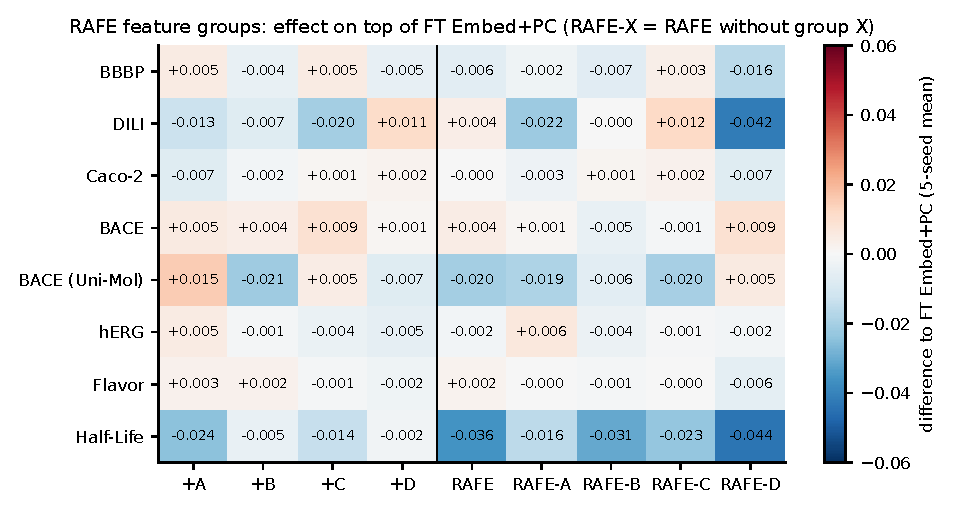
\includegraphics[width=0.99\textwidth]{ablation_groups_v3.pdf}
  \caption{Change relative to FT Embed+PC for each feature-group arm (RAFE-X: RAFE without group X).}
  \label{fig:groups}
\end{figure}

\begin{figure}[!ht]
  \centering
  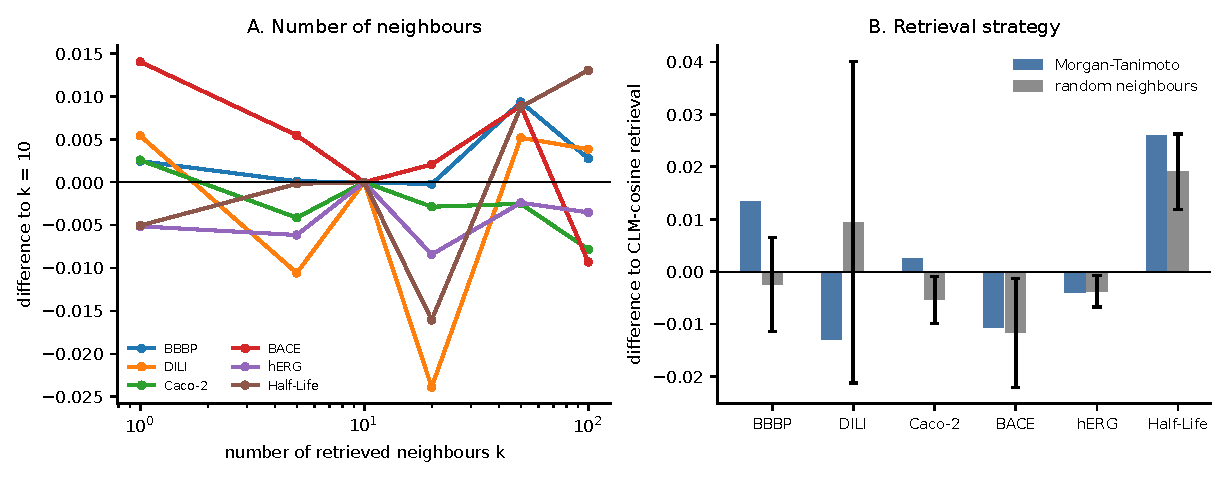
\includegraphics[width=0.99\textwidth]{retrieval_robustness_v3.pdf}
  \caption{Left: effect of the number of retrieved neighbors (difference to $k=10$). Right: effect of the retrieval strategy (difference to CLM-cosine retrieval; error bars show the spread over the five random draws).}
  \label{fig:retrieval}
\end{figure}

\begin{figure}[!ht]
  \centering
  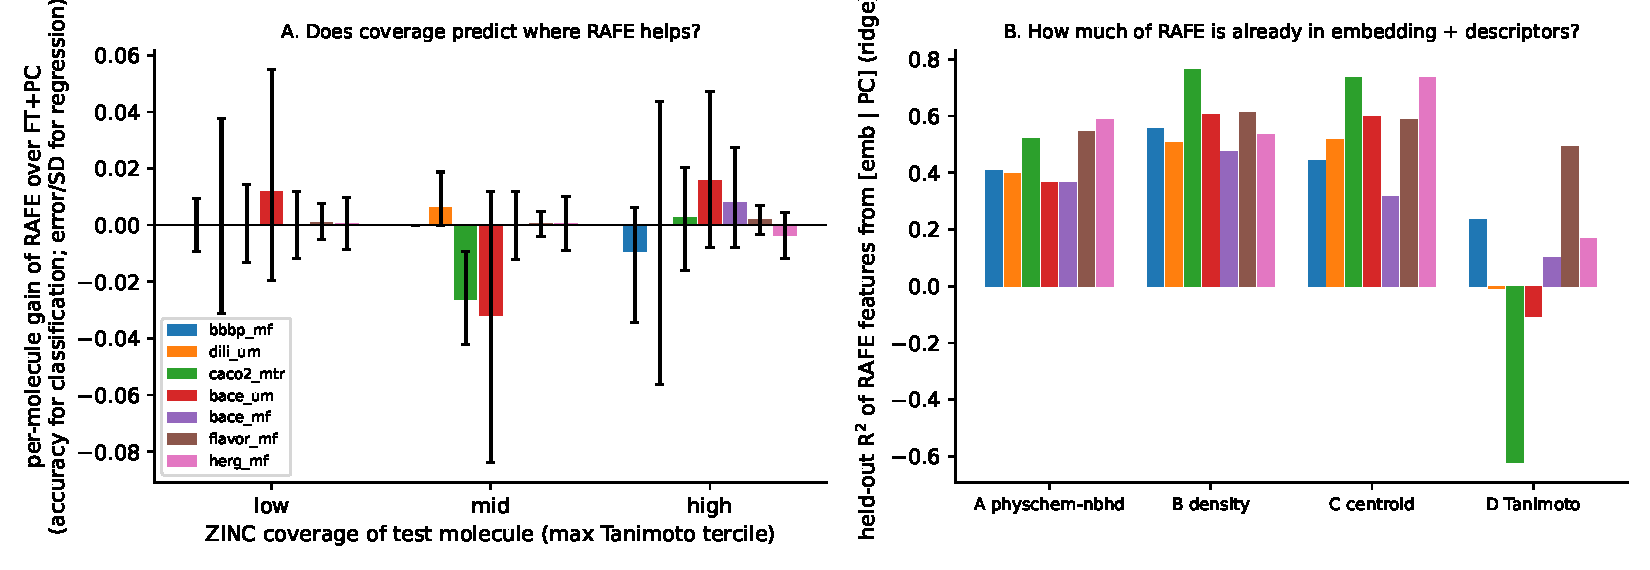
\includegraphics[width=0.99\textwidth]{rafe_complementarity_v3.pdf}
  \caption{Left: per-molecule gain of RAFE over FT Embed+PC by ZINC-250k coverage tercile. Right: held-out R\textsuperscript{2} of each RAFE group predicted from the embedding and the descriptors.}
  \label{fig:e10}
\end{figure}

\begin{table*}[!ht]
\centering
\caption{Label-free RAFE variants at each dataset's configuration (own tree, five-seed test means). The best variant is the one with the highest test mean among RAFE and V1 to V5. Intervals are paired bootstrap 95\% intervals. V1: groups A and B only; V2: residualized features; V3: additional ZINC-250k properties; V4: compressed features; V5: hybrid retrieval.}
\label{tab:variants}
\scriptsize
\adjustbox{max width=\textwidth}{\begin{tabular}{lllllll}
\toprule
Dataset & PC-only & FT+PC & RAFE & Best variant (test mean) & Minus RAFE [95\% CI] & Minus FT+PC [95\% CI] \\
\midrule
BBBP & 0.731 & 0.785 & 0.779 & V1\_AB (0.792) & +0.013 [$-$0.003, +0.036] & +0.007 [$-$0.002, +0.017] \\
DILI & 0.672 & 0.693 & 0.697 & V2\_residual (0.703) & +0.006 [$-$0.041, +0.056] & +0.010 [$-$0.036, +0.063] \\
Caco-2 & 0.833 & 0.813 & 0.817 & V2\_residual (0.820) & +0.003 [$-$0.004, +0.011] & +0.006 [$-$0.000, +0.014] \\
BACE & 0.485 & 0.549 & 0.553 & V5\_hybrid (0.558) & +0.005 [$-$0.020, +0.030] & +0.009 [$-$0.014, +0.033] \\
hERG & 0.577 & 0.545 & 0.544 & V1\_AB (0.551) & +0.007 [$-$0.003, +0.018] & +0.006 [$-$0.003, +0.014] \\
Half-Life & 0.499 & 0.595 & 0.559 & V4\_compressed (0.583) & +0.023 [$-$0.026, +0.072] & $-$0.013 [$-$0.044, +0.020] \\
\bottomrule
\end{tabular}
}
\end{table*}

\subsection{Coverage of the Chemical Space by ZINC-250k}\label{sec:coverage}
For every dataset molecule we computed the largest Morgan-Tanimoto similarity to ZINC-250k (Table~\ref{tab:coverage}, Figure~\ref{fig:umap}). The median is \covmedian{} over all \covn{} molecules, and about \covsixty\% have a neighbor at 0.6 or above; BACE is the least covered (median \covbace{}). ZINC-250k therefore provides background chemical context and not close analogues. This agrees with the result that random neighbors perform like similar ones and that the per-molecule gain does not depend on coverage. Whether a task-matched library would do better is untested.

\begin{table}[!ht]
\centering
\caption{Coverage of the dataset molecules by ZINC-250k (maximum Morgan-Tanimoto similarity).}
\label{tab:coverage}
\small
\adjustbox{max width=\textwidth}{\begin{tabular}{llllll}
\toprule
Dataset & Molecules & Median max Tanimoto to ZINC & Fraction >=0.4 & Fraction >=0.6 & Fraction >=0.8 \\
\midrule
BACE & 1513 & 0.338 & 0.151 & 0.002 & 0.000 \\
BBBP & 1996 & 0.418 & 0.581 & 0.128 & 0.021 \\
Caco-2 & 910 & 0.404 & 0.526 & 0.080 & 0.008 \\
DILI & 475 & 0.425 & 0.587 & 0.135 & 0.013 \\
Flavor & 15025 & 0.431 & 0.624 & 0.070 & 0.006 \\
Half-Life & 654 & 0.407 & 0.526 & 0.104 & 0.015 \\
hERG & 13445 & 0.375 & 0.382 & 0.016 & 0.001 \\
\bottomrule
\end{tabular}
}
\end{table}

\begin{figure}[!ht]
  \centering
  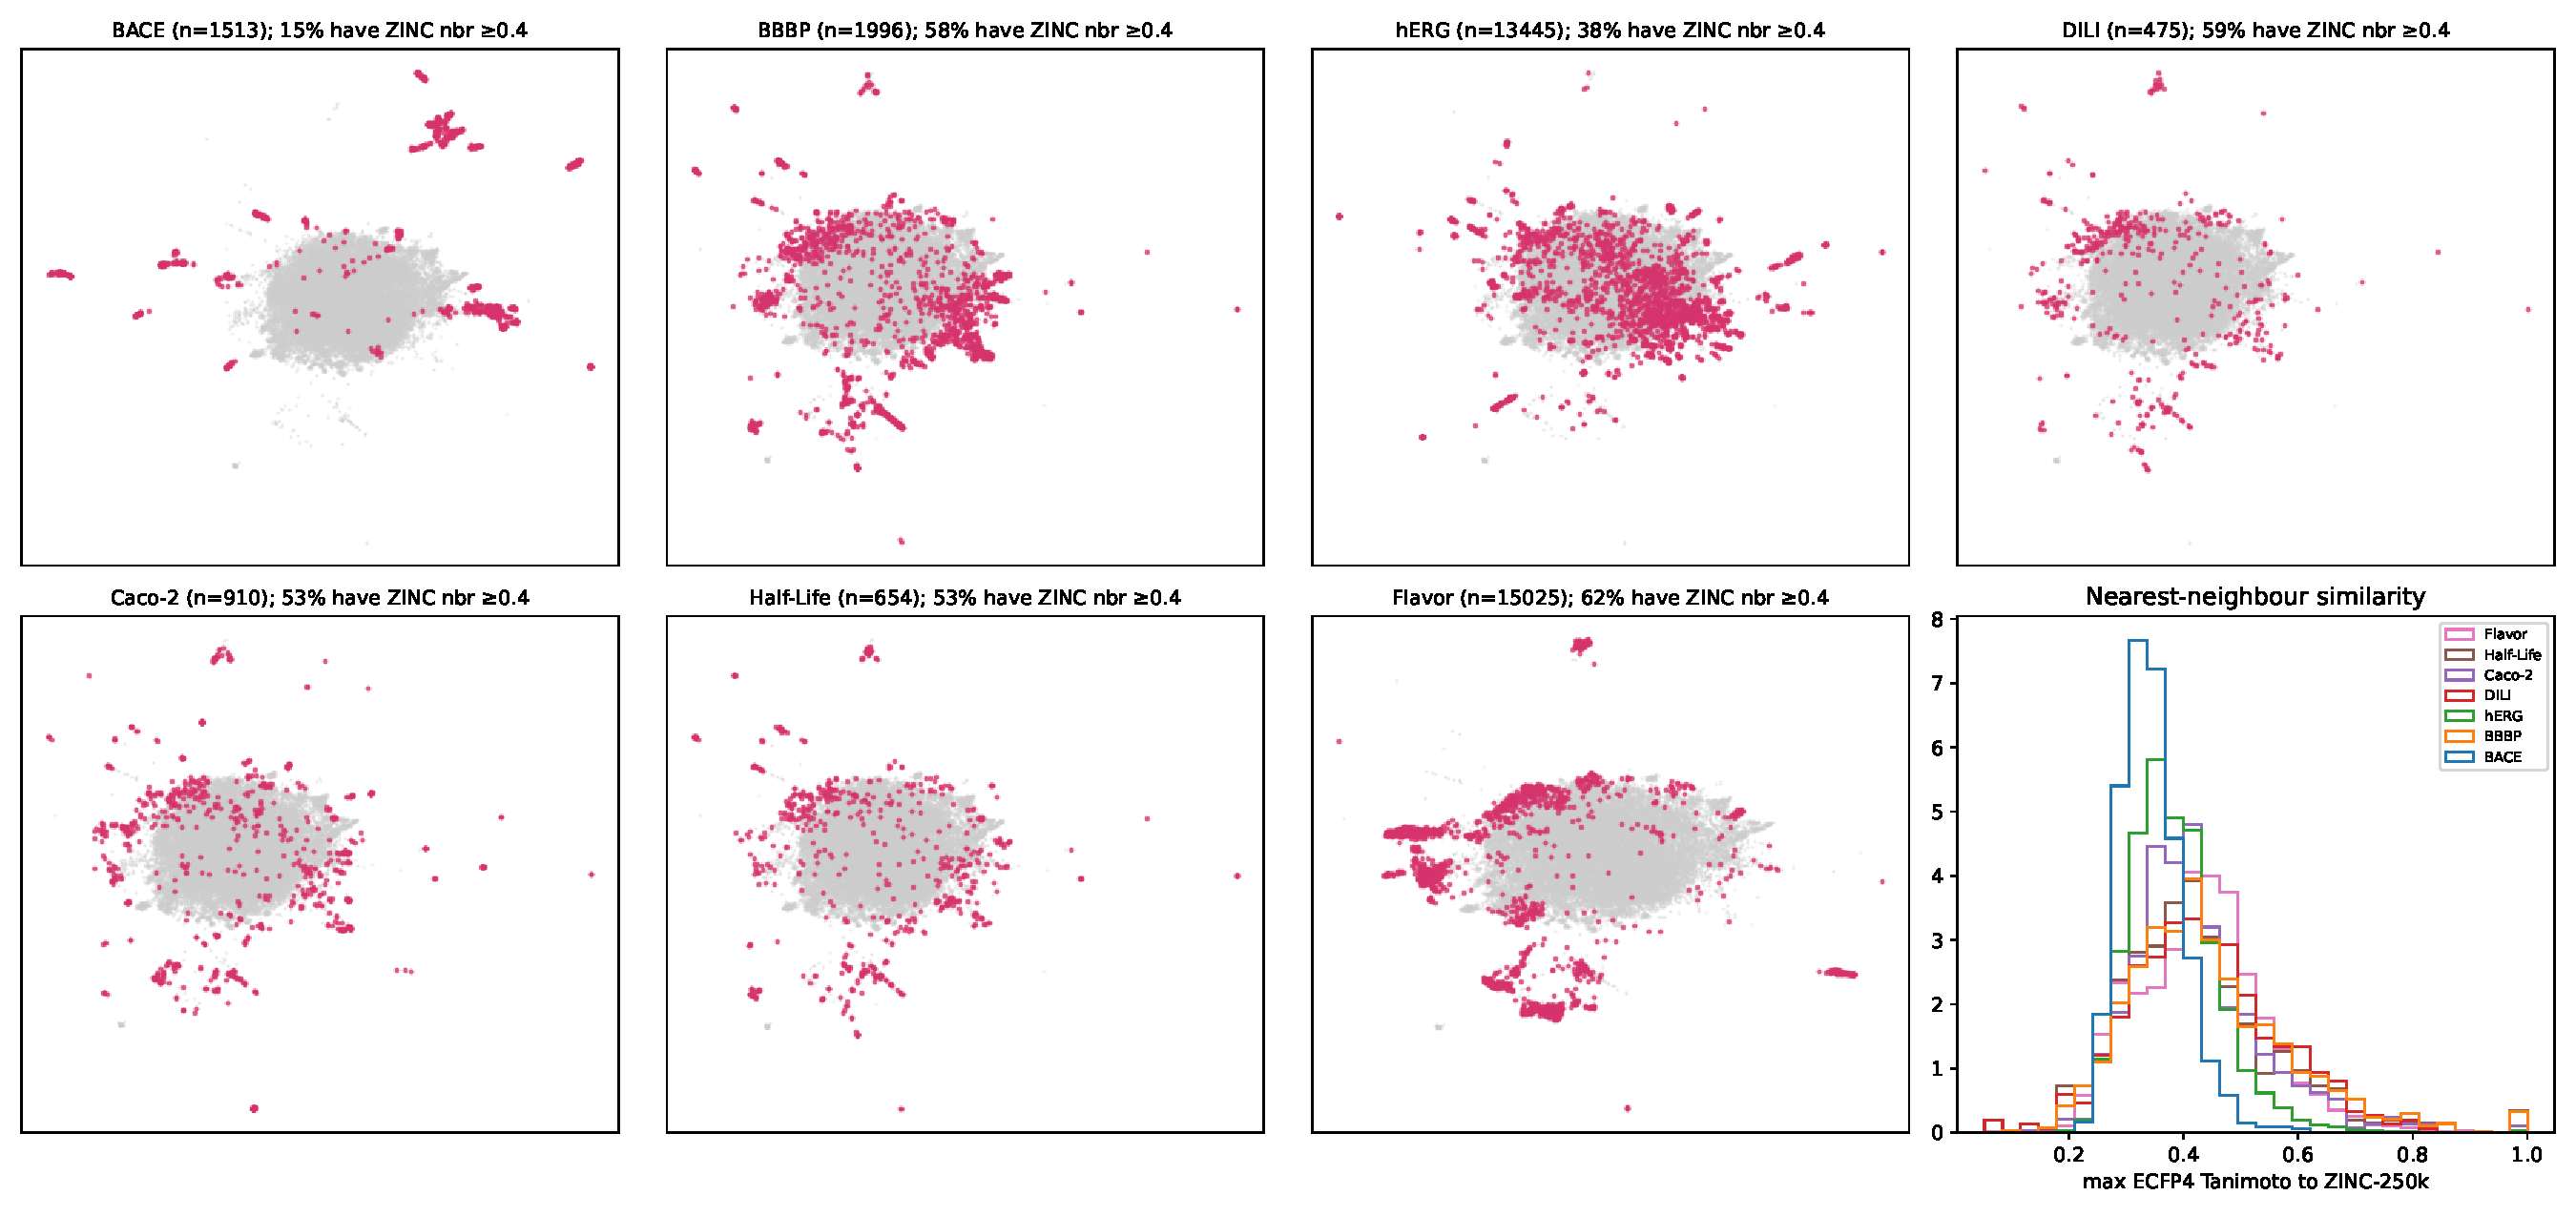
\includegraphics[width=0.8\textwidth]{umap_coverage_v3.pdf}
  \caption{Joint UMAP of the dataset molecules and ZINC-250k.}
  \label{fig:umap}
\end{figure}

\subsection{3D Information, ECFP4 and Conformers}\label{sec:3d_ecfp}
This section addresses H3. The Uni-Mol vector concatenates the 3D encoder output with an ECFP4 fingerprint, so a gain may come from either part. Table~\ref{tab:3d_ecfp} separates the 3D vector, the ECFP4 part and their concatenation with five seeds. On BACE, the ECFP4 part alone scores higher than the 3D vector (\ecfpbace{} versus \threedbace{} with XGBoost; the difference is significant for LightGBM and CatBoost). On Caco-2 the concatenation is clearly better than either part ($+\concatlo$ to $+\concathi$ over the 3D vector for XGBoost and CatBoost), so the two views are complementary there. On DILI the 3D vector outperforms ECFP4 for CatBoost. The headline BACE result (MCC$=0.623$) is the end-to-end LoRA Uni-Mol model with its own head, which does not use ECFP4, so the ECFP4 confound applies only to the frozen-embedding rows.

The conformer also matters. We re-embedded BACE with five RDKit ETKDG seeds (the original seed reproduces the stored embeddings exactly). The 3D vector changes noticeably between conformers (median cosine similarity to the original \coslo{} to \coshi{}). The resulting spread in test MCC is \rthreedlo{} to \rthreedhi{} times the tuning noise for the 3D vector alone and \rcatlo{} to \rcathi{} times with ECFP4 added (Table~\ref{tab:conformers}, Figure~\ref{fig:3d}), so results from a single conformer should be reported with this caveat. Pipelines built on SMILES-based models, including the RAFE configurations with MolFormer and ChemBERTa, involve no conformers. We examined conformers on BACE only.

\begin{table}[!ht]
\centering
\caption{3D versus ECFP4 within the Uni-Mol vector (XGBoost, five seeds; MCC, and Spearman for Caco-2).}
\label{tab:3d_ecfp}
\scriptsize
\adjustbox{max width=\textwidth}{\begin{tabular}{llll}
\toprule
Dataset & 3D vector (512-d) & ECFP4 (2048-bit) & Both (2560-d) \\
\midrule
BACE & 0.394 & 0.495 & 0.429 \\
BBBP & 0.690 & 0.694 & 0.721 \\
Caco-2 & 0.522 & 0.518 & 0.653 \\
DILI & 0.521 & 0.410 & 0.520 \\
\bottomrule
\end{tabular}
}
\end{table}

\begin{table}[!ht]
\centering
\caption{Conformer-seed sensitivity on BACE (five conformer seeds times three tree seeds).}
\label{tab:conformers}
\scriptsize
\adjustbox{max width=\textwidth}{\begin{tabular}{llllll}
\toprule
Input & Tree & Mean MCC & \shortstack{SD across 5\\conformer seeds} & \shortstack{SD across 3\\tree seeds} & \shortstack{Range over\\conformers} \\
\midrule
3D vector (512-d) & LightGBM & 0.363 & 0.042 & 0.011 & 0.096 \\
3D vector (512-d) & XGBoost & 0.349 & 0.045 & 0.006 & 0.099 \\
3D + ECFP4 (2560-d) & LightGBM & 0.428 & 0.024 & 0.011 & 0.063 \\
3D + ECFP4 (2560-d) & XGBoost & 0.411 & 0.022 & 0.007 & 0.049 \\
\bottomrule
\end{tabular}
}
\end{table}

\begin{figure}[!ht]
  \centering
  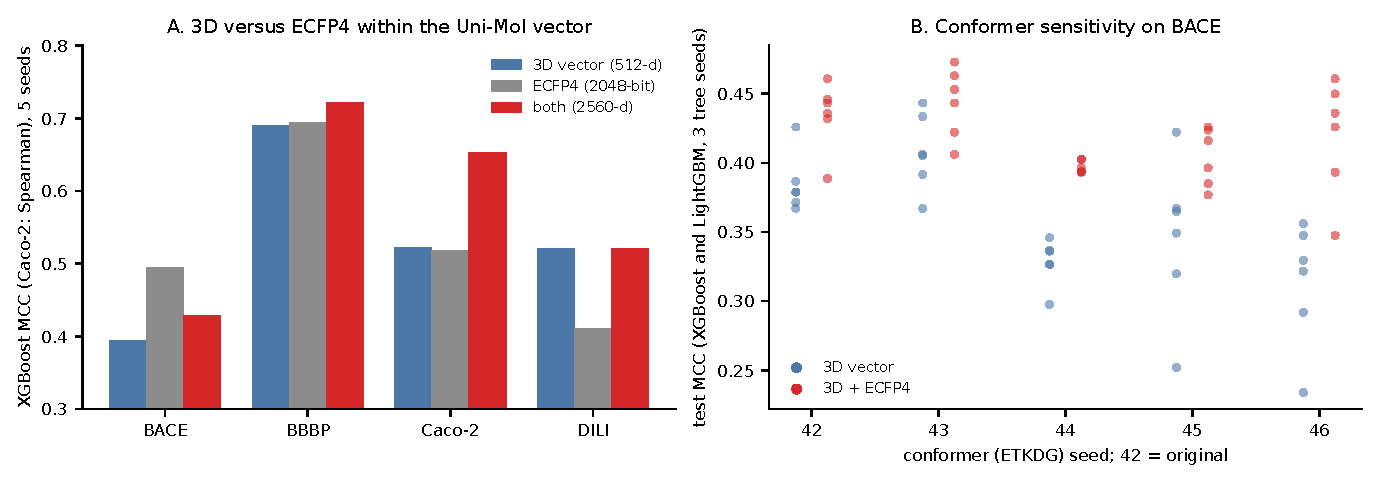
\includegraphics[width=0.99\textwidth]{3d_ecfp4_conformers_v3.pdf}
  \caption{Left: 3D vector versus ECFP4 versus both (XGBoost). Right: test MCC for each conformer seed (42 is the original), both inputs, XGBoost and LightGBM.}
  \label{fig:3d}
\end{figure}

\subsection{Efficiency Analysis}\label{sec:efficiency}
Table~\ref{tab:params} reports LoRA hyperparameters and trainable parameter counts illustrating the range of parameter efficiency across five of the seven datasets. ChemBERTa variants (3.4M base parameters) achieve reductions of $76$-$94\%$ depending on rank; MolFormer-XL ($\approx 46$M parameters) achieves $84$-$97\%$ reduction. Uni-Mol (rank $r \in \{4,8,16,32\}$, targeting only \texttt{in\_proj} across 15 attention layers) achieves particularly efficient adaptation, with $<5\%$ trainable parameters for the lowest-rank configurations. hERG (MolFormer-XL, $r=16$) reduces parameters by $93.91\%$, and DILI (ChemBERTa-MTR, $r=64$) by $76.31\%$. Both fall within the same $76$-$97\%$ range observed elsewhere in the table. The full parameter counts for BACE, BBBP and Flavor datasets are in Supplementary Table~S9. This addresses H1: LoRA reduces the trainable parameters by $76$-$97\%$, and the end-to-end LoRA results are competitive with the published full-finetuning and graph baselines (Section~\ref{sec:external_comparison}).

\paragraph{Computational cost.} Table~\ref{tab:runtime} and Figure~\ref{fig:runtime} give the cost of each stage, measured or taken from the logs of the original runs. One-off costs are small for the SMILES models (LoRA finetuning: median \lorarun{}; embedding the 249k-molecule library: about \zhmin{} minutes) and large for Uni-Mol (hours, dominated by conformer generation: \umhours{}). At prediction time RAFE adds about \raferq{} s for a single molecule on a shared GPU with exact search, and tree inference takes under a millisecond. The numbers come from different hardware and are indicative.

\begin{table}[!ht]
\centering
\caption{Runtime of the pipeline stages.}
\label{tab:runtime}
\scriptsize
\adjustbox{max width=\textwidth}{\begin{tabular}{lll}
\toprule
Stage & Cost & Source \\
\midrule
LoRA fine-tuning, one run & median 13 s, IQR 6-43 s, max 540 s & training logs; lower bound \\
Library embedding, SMILES models (6 variants) & 4.4 min (hERG), 4.2 min (DILI) & original run logs \\
Library embedding, Uni-Mol & herg: 8.4 h, dili: 9.1 h, caco2: 1.7 h & original run logs \\
RAFE at inference, one molecule & retrieval 125.8 ms, features 3.8 ms, total 129.6 ms (129.63 ms per molecule) & measured, shared P100, exact search \\
RAFE at inference, 192 molecules & retrieval 139.8 ms, features 456.2 ms, total 596.0 ms (3.10 ms per molecule) & measured \\
XGBoost inference, one molecule & 0.5 ms & measured \\
Tree stage per cell (20 trials, 5-fold CV, fit) & XGBoost median 639 s, IQR 398-888 s; LightGBM median 213 s, IQR 33-778 s; CatBoost median 1560 s, IQR 833-4380 s & loaded shared server; upper bound \\
\bottomrule
\end{tabular}
}
\end{table}

\begin{figure}[!ht]
  \centering
  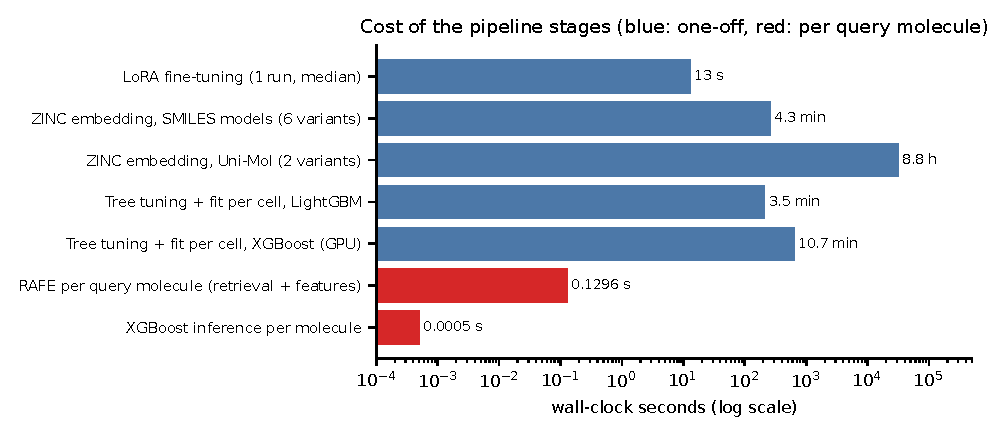
\includegraphics[width=0.8\textwidth]{runtime_v3.pdf}
  \caption{Cost of the pipeline stages (blue: one-off; red: per query molecule).}
  \label{fig:runtime}
\end{figure}

\begin{table}[!ht]
\centering
\caption{Selected LoRA configurations illustrating the range of parameter efficiency. Trainable~\% = 100 $\times$ trainable / (total parameters + trainable).}
\label{tab:params}
\begin{tabular}{llllrrrr}
\toprule
Dataset & Model & $r$ & $\alpha$ & Total & Trainable & Trainable \% & \% Reduction \\
\midrule
BACE   & ChemBERTa-MLM & 4  & 32  & 3.43M & 205K  & 5.66  & 94.34 \\
BACE   & MolFormer-XL  & 64 & 128 & 45.6M & 8.26M & 15.35 & 84.65 \\
BBBP   & ChemBERTa-MLM & 64 & 32  & 3.43M & 1.06M & 23.69 & 76.31 \\
BBBP   & MolFormer-XL  & 32 & 8   & 45.6M & 4.72M & 9.39  & 90.61 \\
Flavor & MolFormer-XL  & 4  & 64  & 45.6M & 1.63M & 3.44  & 96.56 \\
hERG   & MolFormer-XL  & 16 & 64  & 45.6M & 2.95M & 6.09  & 93.91 \\
DILI   & ChemBERTa-MTR & 64 & 128 & 3.43M & 1.06M & 23.69 & 76.31 \\
\bottomrule
\end{tabular}
\end{table}

Parameter efficiency is a design property, not a per-run measurement, so it is reported once here rather than repeated per dataset. Because LoRA reduces trainable parameters without any corresponding loss in accuracy across the seven datasets studied, the parameter savings in Table~\ref{tab:params} translate directly into lower fine-tuning memory footprint and training cost relative to full-parameter finetuning of the same backbones, at effectively no cost to the reported MCC/Spearman scores.

\subsection{Comparison with External Baselines}\label{sec:external_comparison}
Table~\ref{tab:external_main} compares the best PEARL configurations against published graph-based and language-model baselines on BACE, BBBP, and Flavor, the three MoleculeNet-era datasets for which comparable external LoRA/GNN literature numbers exist. AUC is the primary comparison metric as it is most consistently reported across sources. The full method description is available in Supplementary Section~S5 (see Supplementary Table~S11). The four TDC ADMET datasets have no directly comparable published LoRA baseline, so for those datasets PC-only, Chemprop, and GCN, all run in-house on the identical split, serve as the reference comparison.

\begin{table*}[!ht]
\centering
\caption{AUC comparison with published external baselines on MoleculeNet scaffold splits (BACE/BBBP/Flavor only). \textsuperscript{a}~Mean~$\pm$~std over multiple seeds (cited source). \textsuperscript{b}~PEARL point estimate. ``-''~= not reported.}
\label{tab:external_main}
\resizebox{0.95\textwidth}{!}{
\begin{tabular}{llccc}
\toprule
\textbf{Method} & \textbf{Ref.} & \textbf{BACE} & \textbf{BBBP} & \textbf{Flavor} \\
\midrule
\multicolumn{5}{l}{\textit{Graph neural network baselines (published)}} \\[2pt]
Chemprop (D-MPNN)      & \cite{yang2019chemprop}  & $0.861 \pm 0.034$\textsuperscript{a} & $0.919 \pm 0.026$\textsuperscript{a} & --- \\
GROVER-Large           & \cite{rong2020grover}    & $0.894 \pm 0.028$\textsuperscript{a} & $0.940 \pm 0.016$\textsuperscript{a} & --- \\
Mole-BERT              & \cite{xia2023molecbert}  & $0.856 \pm 0.029$\textsuperscript{a} & $0.940 \pm 0.011$\textsuperscript{a} & --- \\
\midrule
\multicolumn{5}{l}{\textit{Graph neural network baselines (this work, in-house)}} \\[2pt]
Chemprop    & this work & $0.855$\textsuperscript{b} & $0.918$\textsuperscript{b} & $0.974$\textsuperscript{b} \\
GCN (in-house)         & this work & $0.795$\textsuperscript{b} & $0.924$\textsuperscript{b} & $0.973$\textsuperscript{b} \\
\midrule
\multicolumn{5}{l}{\textit{Chemical language models (full finetuning, published)}} \\[2pt]
Uni-Mol (full FT)      & \cite{zhou2023unimol}    & $0.857 \pm 0.002$\textsuperscript{a} & $0.932 \pm 0.003$\textsuperscript{a} & --- \\
MolFormer-XL (full FT) & \cite{ross2022molformer} & ---                                  & $0.932$\textsuperscript{a}           & --- \\
FART model             & \cite{zimmermann2024fart}& ---                                  & ---                                  & $0.964$ \\
\midrule
\multicolumn{5}{l}{\textit{PEARL (this work, LoRA finetuning)}} \\[2pt]
PEARL Uni-Mol WL (E2E LoRA)   & this work & $\mathbf{0.891}$\textsuperscript{b} & $0.943$\textsuperscript{b}          & $0.973$\textsuperscript{b} \\
PEARL MolFormer FL (E2E LoRA) & this work & $0.872$\textsuperscript{b}          & $0.929$\textsuperscript{b} & $\mathbf{0.975}$\textsuperscript{b} \\
PEARL RAFE best               & this work & $0.858$\textsuperscript{b}          & $\mathbf{0.940}$\textsuperscript{b}          & $0.963$\textsuperscript{b} \\
\midrule
\multicolumn{5}{l}{\textit{PC-only (this work, no CLM)}} \\[2pt]
PC-only (in-house)     & this work & $0.850$\textsuperscript{b}          & $0.937$\textsuperscript{b}          & $0.972$\textsuperscript{b} \\
\bottomrule
\end{tabular}
}
\end{table*}

On \textbf{BACE}, PEARL Uni-Mol WL (AUC~$=0.891$) is competitive with GROVER-Large ($0.894\pm0.028$) within the reported standard deviation, and surpasses both the published Uni-Mol full-finetuning result ($0.857$) and the in-house Chemprop/GCN baselines ($\le0.855$). On \textbf{BBBP}, PEARL MolFormer E2E LoRA (AUC~$=0.929$) and RAFE (AUC$=0.940$) both exceed the in-house GCN (AUC$=0.924$) and Chemprop (AUC$=0.918$) baselines, and RAFE exceeds GROVER-Large and Mole-BERT (both $0.940$, tied). On \textbf{Flavor}, in-house Chemprop (AUC$=0.974$) is essentially tied with PEARL MolFormer E2E LoRA ($0.975$): the CLM ladder's margin over a graph-only baseline is negligible on this dataset, consistent with the earlier PC-only finding.

\subsection{Discussion}\label{sec:bace_discussion}
Across seven datasets and two task types, PEARL holds every claimed improvement to in-house, identically evaluated baselines and reports where the improvements disappear.

\textbf{H1 (parameter efficiency).} LoRA reduces the trainable parameters by $76$-$97\%$ while the end-to-end models remain competitive with published full-finetuning and graph baselines. This claim rests on the parameter counts (Table~\ref{tab:params}) and on the external comparison (Table~\ref{tab:external_main}).

\textbf{H2 (information added by retrieval).} RAFE is a safe and inexpensive final stage. It improves on the fine-tuned embedding alone on four datasets, it is never significantly different from the embedding plus descriptors in the controlled matrix, and its settings need no tuning. The evidence does not support a general advantage over embedding plus descriptors. Where the grid shows an advantage, it depends on the tree: on DILI with XGBoost RAFE exceeds FT Embed+PC, but with LightGBM the difference disappears. On five-seed means, RAFE's best configuration ranks in the top three of seven methods on \ntop{} of \nds{} datasets, behind FT Embed+PC on average. Random neighbors work as well as similar ones, the gain is unrelated to ZINC-250k coverage, and no label-free variant improves on RAFE, so we interpret RAFE as chemical-space context that largely overlaps with the embedding and descriptors.

\textbf{PC-only is a strong baseline.} A tree ensemble on 473 engineered descriptors is the highest-scoring or tied method on Caco-2, hERG and Flavor, and it is significantly above RAFE on hERG (all three trees) and on Flavor (XGBoost). We report this because it is the central question of the benchmark: does the added complexity of CLM finetuning, LoRA adaptation and retrieval earn its keep over a simple, interpretable tree ensemble? Dataset by dataset, the answer is sometimes, and where it does, the gain is modest. We recommend a PC-only baseline as a standard control in molecular CLM benchmarks.

\textbf{H3 (3D geometry).} Uni-Mol with end-to-end LoRA gives the highest single-run BACE result (MCC$=0.623$), consistent with the dependence of BACE-1 inhibition on three-dimensional complementarity. Our data do not show that the model captures protein-ligand interactions. The frozen Uni-Mol vector contains an ECFP4 block, and on BACE the ECFP4 part alone scores higher than the 3D vector. The 3D vector also depends on the conformer. A 3D architecture helps on BACE, but the evidence for geometry as the cause is indirect.

\textbf{Task-dependent choices persist.} MolFormer is the best embedding in \nmf{} of \nrows{} rows of Table~\ref{tab:best_configs}. The best loss varies: focal loss in the best configurations of BBBP and DILI, weighted loss on BACE. On the five datasets with a complete grid, adding PC features to the fine-tuned embedding helps mainly on Caco-2 ($+0.086$ on average over configurations) and DILI ($+0.044$) and by at most $0.01$ elsewhere.

\subsection{Interpreting the Performance Metrics}\label{sec:metrics}
Three examples show how the choice of metric changes the conclusion. On BBBP, the effect of RAFE over FT Embed+PC depends on the tree (\bbbcat{} with CatBoost, \bbblgb{} with LightGBM and \bbbxgb{} with XGBoost; Table~\ref{tab:controlled}), so we describe it as small and tree-dependent. On DILI, the best configuration depends on the metric. For RAFE, MCC, accuracy and F1 select \dilirafecfg{} (MCC \dilirafemcc{}), whereas AUC selects \dilirafeaucfg{} (\dilirafeauc{}). The rank correlation between MCC and AUC across configurations is \rhomcclo{} to \rhomcchi{}. With 96 test molecules, MCC at a fixed threshold is noisier than AUC, so we state the ranking metric and report AUC alongside. On Half-Life, Spearman correlation and R\textsuperscript{2} behave differently because R\textsuperscript{2} is computed in hours after inverting the log1p transform, where \sharethree\% of the test variance sits in three molecules (Figure~\ref{fig:halflife}). For the fingerprint and descriptor baselines, R\textsuperscript{2} rises from \rawr{} in hours to \logr{} on the log scale. The rank correlation between Spearman and R\textsuperscript{2} across the supplementary configurations is \rhoall{} (\rhorafe{} within RAFE). The models rank half-lives moderately well (Spearman \spbestlo{} to \spbesthi{} for the best configuration of each stage) but do not predict their magnitude.

\begin{figure}[!ht]
  \centering
  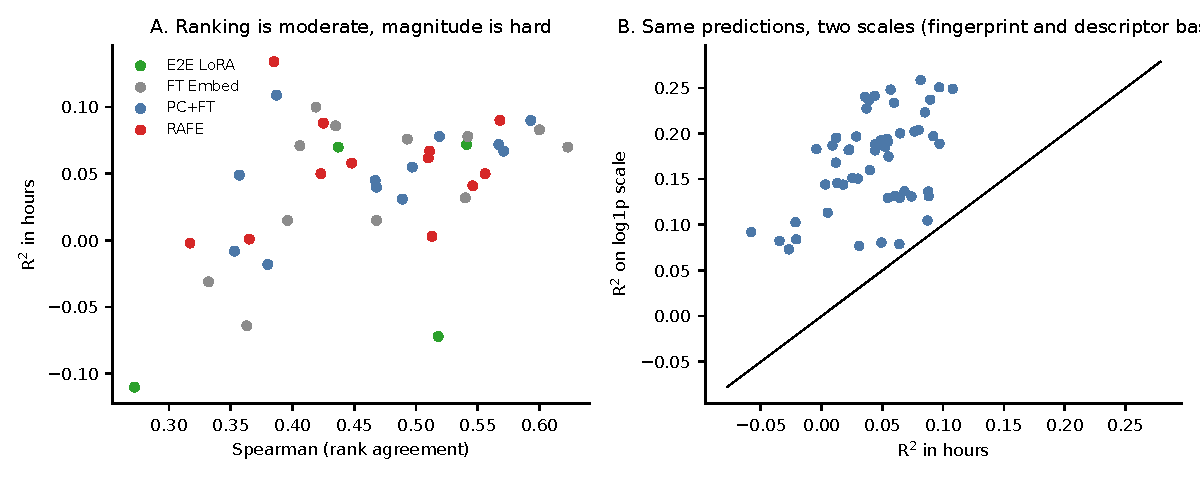
\includegraphics[width=0.99\textwidth]{halflife_metrics_v3.pdf}
  \caption{Half-Life. Left: Spearman versus R\textsuperscript{2} (hours) over the supplementary configurations. Right: R\textsuperscript{2} in hours versus on the log1p scale for the descriptor and fingerprint baselines.}
  \label{fig:halflife}
\end{figure}

%% =====================================================================
\section{Conclusion and Future Work}\label{sec:conclusion}

PEARL provides a uniform benchmark of parameter-efficient adaptation of 1D and 3D chemical language models, with retrieval-augmented features and in-house descriptor, fingerprint and graph baselines, on seven classification and regression datasets. LoRA reduces the trainable parameters by $76$-$97\%$ at competitive accuracy. RAFE improves on the fine-tuned embedding alone on four datasets but is never significantly different from embedding plus descriptors in the controlled comparison, and a descriptor-only baseline is the strongest or tied method on three datasets. End-to-end LoRA on Uni-Mol gives the best single-run BACE result (MCC$=0.623$). We conclude that RAFE is a safe, inexpensive final stage with modest, dataset-specific value, and that the strength of the descriptor baseline should shape how CLM benchmarks are reported.

\subsection{Limitations}\label{sec:limitations}
Several limitations apply. First, seed variability covers the downstream tree stage; LoRA finetuning and the re-embedding of ZINC-250k were not repeated with independent seeds, and the end-to-end LoRA, Chemprop and GCN baselines are single runs, so our intervals are lower bounds on the total variability. Second, the best configuration is chosen on the test set, as is usual for benchmarks, and is therefore optimistic; five-seed means and paired differences to the runner-up quantify this, but an external test set would be needed to remove it. Third, several test sets are small (DILI $n=96$; Caco-2 $n=182$; Half-Life $n=133$; BACE $n\approx152$), which widens intervals. Fourth, ZINC-250k covers the task chemistry only moderately (median maximum Tanimoto similarity \covmedian{}), and other libraries were not tested. Fifth, conformer sensitivity was examined on BACE only. Sixth, the new experiments ran XGBoost on GPU, so absolute values differ slightly from the original CPU runs, and arms are compared within experiments. Seventh, a training molecule's embedding comes from an encoder finetuned on that molecule, which can favor overfitting in frozen-embedding models. \pending{state which full-grid results (CatBoost, hERG, Flavor) are included in this version}

\subsection{Future Directions}\label{sec:future_work}
A task-matched retrieval library, and retrieval that uses labels only from the training split under a leakage-free protocol, would test whether RAFE's gain grows when the neighbors are closer to the task chemistry. Repeating LoRA finetuning with independent seeds would complete the variability estimate. Extending the regression support with calibrated uncertainty (quantile regression or conformal prediction on the tree stage) would make the Caco-2 and Half-Life results more actionable. Emerging multi-modal CLMs such as nach0~\cite{livne2024nach0} and Omni-Mol~\cite{hu2025omnimol} are natural extensions of the LoRA and RAFE approach. Finally, given how often PC-only competes with the CLM ladder here, future benchmarks of molecular CLMs should treat a PC-only baseline as a mandatory control.

%%=====================================================
\section*{Key Points}
\begin{itemize}

\item PEARL applies LoRA to three chemical language models (ChemBERTa, MolFormer, Uni-Mol) and adds RAFE, a retrieval stage that summarizes the ZINC-250k neighborhood of each molecule with 60 label-free features.
\item Seven datasets (binary, multi-class and regression) are evaluated under one protocol with three tree models, five seeds, tuning on the training split only, and paired bootstrap intervals.
\item RAFE improves on the fine-tuned embedding alone on four datasets but is never significantly different from embedding plus descriptors in 24 paired comparisons.
\item A descriptor-only baseline with no language model is the strongest or tied method on Caco-2, hERG and Flavor, and should be a standard control in molecular CLM benchmarks.
\item End-to-end LoRA on Uni-Mol gives the best single-run BACE result (MCC = 0.623), but the Uni-Mol vector contains an ECFP4 block and depends on the conformer.

\end{itemize}
%%%%%%%%%%%%%%%%%%%%%%%%%%%%%%%%%%%%%%%%%%%%%%%%%%%%%%%%
\backmatter

%% =====================================================================
\section*{Declarations}

\begin{itemize}
\item Funding Sources

This research did not receive any specific grant from funding agencies in the public, commercial, or not-for-profit sectors.

\item Competing interests

The authors declare no competing financial interests. R.M.\ is Scientific Advisor at Eternal, U.A.E.

\item Data availability

All code and data associated with PEARL, including the TDC data-curation, RAFE, and in-house GNN baseline pipelines, is available at \url{https://github.com/raghvendra5688/PEARL}.

\item Acknowledgments

We thank the Qatar National Library (QNL) for their support in providing resources and funding the APC.

\item Author contributions

K.A. contributed to Methods, Experiments, Validation, Writing (original draft). S.G. and H.B. participated in Project Supervision, Methods, Writing (review \& editing). Y.Z. and C.Y. participated in Project Supervision, Writing (review \& editing). R.M. conceptualized and supervised the project, and contributed to Methods, Experiments, Validation, Writing (review \& editing).

\item{Declaration of generative AI and AI-assisted technologies in the writing process}

During the preparation of this work the authors used ChatGPT (OpenAI) and Claude (Anthropic) to assist with phrasing, grammar correction, and refinement of English expressions in the manuscript. In the revision, Claude Code (Anthropic) was also used to help write and run analysis scripts and to edit the text, and an editing guideline for academic prose (academic-humanizer) was applied to improve clarity. All numbers, tables and figures were generated from the result files and checked by the authors. After using these tools, the authors reviewed and edited the content as needed and take full responsibility for the content of the publication. \pending{authors to confirm the wording against the journal's AI-use policy}

\item{Supplementary information}

The supplementary material accompanying this article contains additional experimental details, complete ablation studies, feature descriptions, and implementation details supporting the results presented in the main manuscript.

\end{itemize}

\section*{Supplementary Material}\label{sec:supplementary}

\noindent\textbf{Supplementary Table S1.} RDKit-derived molecular descriptors, NetworkX graph features, Morgan fingerprints, and MACCS keys comprising the 473-dimensional engineered feature vector.

\noindent\textbf{Supplementary Table S2.} Full BBBP ablation: all modality $\times$ CLM $\times$ loss $\times$ ML combinations.

\noindent\textbf{Supplementary Table S3.} Full Flavor ablation including per-class AUPR.

\noindent\textbf{Supplementary Table S4.} Full BACE ablation.

\noindent\textbf{Supplementary Table S5.} Full hERG ablation (TDC ADMET Group).

\noindent\textbf{Supplementary Table S6.} Full DILI ablation (TDC ADMET Group).

\noindent\textbf{Supplementary Table S7.} Full Caco-2 ablation, regression (TDC ADMET Group).

\noindent\textbf{Supplementary Table S8.} Full Half-Life ablation, regression (TDC ADMET Group).

\noindent\textbf{Supplementary Table S9.} Complete LoRA parameter efficiency analysis for all model families, datasets (including the four TDC ADMET datasets), and loss functions.

\noindent \textbf{Supplementary Table S10.} RAFE feature vector composition (60 features: 18 physicochemical neighborhood, 5 density, 34 centroid, 3 Tanimoto).

\noindent \textbf{Supplementary Table S11.} Comparison of PEARL with published external baselines on MoleculeNet scaffold splits (BACE/BBBP/Flavor only).

\noindent \textbf{Supplementary Table S12.} In-house PC-only/Chemprop/GCN baselines vs. the best CLM-based method, all seven datasets.

\noindent \textbf{Supplementary Table S13.} Full same-tree comparison tables for BACE and Half-Life (layout of Tables~\ref{tab:full_dili} to~\ref{tab:full_bbbp}), and the grid means for every dataset.

\noindent \textbf{Supplementary Table S14.} Paired bootstrap intervals for all controlled comparisons (PC-only, FT Embed, FT Embed+PC and RAFE; fingerprint baselines; retrieval controls; $k$ sweep; 3D versus ECFP4).

\noindent \textbf{Supplementary Table S15.} Per-variant results and paired intervals for the label-free RAFE variants, both trees.

\noindent \textbf{Supplementary Table S16.} Corrections to the previous version of the manuscript and supplement (RAFE feature count, embedding dimensions, LoRA initialization and scaling, loss definitions, BACE configuration label).

\noindent\textbf{Supplementary Section S1.} Zero-shot vs.\ full finetuning: background and comparison.

\noindent\textbf{Supplementary Section S2.} Detailed LoRA mathematical formulation and implementation for Uni-Mol.

\noindent\textbf{Supplementary Section S3.} PEARL custom trainer: loss function implementations (including Huber loss for regression), class-weight computation, and evaluation metric computation.

\noindent\textbf{Supplementary Section S4.} RAFE pipeline details: ZINC-250k cleaning procedure, per-dataset FAISS index construction, PCA fitting strategy, and per-group feature breakdown.

\noindent\textbf{Supplementary Section S5.} Comparison with published external baselines (BACE/BBBP/Flavor) and full description of the in-house Chemprop/GCN/PC-only baseline protocol applied to all seven datasets.

\section*{Appendix}

\bmhead{List of Abbreviations}

\begin{table*}[!ht]
\begin{adjustbox}{max width=0.9\textwidth}
\begin{tabular}{ll}
\toprule
Abbreviation & Expansion \\
\midrule
ADMET & Absorption, Distribution, Metabolism, Excretion, and Toxicity \\
AUC & Area Under the (ROC) Curve \\
Acc & Accuracy \\
BACE & $\beta$-secretase (BACE-1) inhibition dataset \\
BBBP & Blood-Brain Barrier Penetration \\
CI & Confidence Interval \\
CLM(s) & Chemical Language Model(s) \\
DILI & Drug-Induced Liver Injury \\
E2E & End-to-End \\
ECFP4 & Extended-Connectivity (Morgan) Fingerprint, radius $=2$ \\
FART & Flavor Analysis and Recognition Transformer \\
FL & Focal Loss \\
FT Embed & Finetuned Embedding (Prediction) \\
GCN & Graph Convolutional Network \\
GNN(s) & Graph Neural Network(s) \\
LoRA & Low-Rank Adaptation \\
MACCS & Molecular ACCess System (keys) \\
MAE & Mean Absolute Error \\
MCC & Matthews Correlation Coefficient \\
MLM & Masked Language Modeling \\
MTR & Multi-Task Regression \\
PC & Physicochemical \\
PEFT & Parameter-Efficient Finetuning \\
Prec / Rec & Precision / Recall \\
QED & Quantitative Estimate of Drug-likeness \\
QSAR & Quantitative Structure-Activity Relationship \\
RAFE & Retrieval-Augmented Feature Enhancement \\
SAS & Synthetic Accessibility Score \\
SE & Standard Error \\
SMILES & Simplified Molecular Input Line Entry System \\
TDC & Therapeutics Data Commons \\
WL & Weighted (Cross-Entropy) Loss \\
hERG & Cardiac ion-channel inhibition (hERG) dataset \\
\bottomrule
\end{tabular}
\end{adjustbox}
\end{table*}


\footnotesize{
\bibliography{sn-bibliography}
}

\end{document}